\documentclass[titlepage,numbers=noenddot,headinclude,
                footinclude=true,abstractoff,
                BCOR=5mm,paper=letter,fontsize=11pt,
                ngerman,american,dottedtoc]{scrreprt}

% ****************************************************************************************************
% classicthesis-config.tex
% formerly known as loadpackages.sty, classicthesis-ldpkg.sty, and classicthesis-preamble.sty
% Use it at the beginning of your ClassicThesis.tex, or as a LaTeX Preamble
% in your ClassicThesis.{tex,lyx} with \input{classicthesis-config}
% ****************************************************************************************************
% If you like the classicthesis, then I would appreciate a postcard.
% My address can be found in the file ClassicThesis.pdf. A collection
% of the postcards I received so far is available online at
% http://postcards.miede.de
% ****************************************************************************************************


% ****************************************************************************************************
% 0. Set the encoding of your files. UTF-8 is the only sensible encoding nowadays. If you can't read
% äöüßáéçèê∂åëæƒÏ€ then change the encoding setting in your editor, not the line below. If your editor
% does not support utf8 use another editor!
% ****************************************************************************************************
\PassOptionsToPackage{utf8}{inputenc}
	\usepackage{inputenc}
%\usepackage{tikz}
% ****************************************************************************************************
% 1. Configure classicthesis for your needs here, e.g., remove "drafting" below
% in order to deactivate the time-stamp on the pages
% ****************************************************************************************************
\PassOptionsToPackage{eulerchapternumbers,listings,%
					 pdfspacing,floatperchapter,%linedheaders,%
					 subfig,beramono,eulermath,parts}{linux_introduction}
% ********************************************************************
% Available options for classicthesis.sty
% (see ClassicThesis.pdf for more information):
% drafting
% parts nochapters linedheaders
% eulerchapternumbers beramono eulermath pdfspacing minionprospacing
% tocaligned dottedtoc manychapters
% listings floatperchapter subfig
% ********************************************************************


% ****************************************************************************************************
% 2. Personal data and user ad-hoc commands
% ****************************************************************************************************
\newcommand{\myTitle}{Introduction to Linux\xspace}
\newcommand{\mySubtitle}{An Homage to The Elements of Typographic Style\xspace}
\newcommand{\myDegree}{Doktor-Ingenieur (Dr.-Ing.)\xspace}
\newcommand{\myName}{Marcel Jar\xspace}
\newcommand{\myProf}{Put name here\xspace}
\newcommand{\myOtherProf}{Put name here\xspace}
\newcommand{\mySupervisor}{Put name here\xspace}
\newcommand{\myFaculty}{Put data here\xspace}
\newcommand{\myDepartment}{Put data here\xspace}
\newcommand{\myUni}{Put data here\xspace}
\newcommand{\myLocation}{Saarbrücken\xspace}
\newcommand{\myTime}{September 2015\xspace}
\newcommand{\myVersion}{version 4.2\xspace}

% ********************************************************************
% Setup, finetuning, and useful commands
% ********************************************************************
\newcounter{dummy} % necessary for correct hyperlinks (to index, bib, etc.)
\newlength{\abcd} % for ab..z string length calculation
\providecommand{\mLyX}{L\kern-.1667em\lower.25em\hbox{Y}\kern-.125emX\@}
\newcommand{\ie}{i.\,e.}
\newcommand{\Ie}{I.\,e.}
\newcommand{\eg}{e.\,g.}
\newcommand{\Eg}{E.\,g.}
% ****************************************************************************************************


% ****************************************************************************************************
% 3. Loading some handy packages
% ****************************************************************************************************
% ********************************************************************
% Packages with options that might require adjustments
% ********************************************************************
\usepackage{makeidx}
%\PassOptionsToPackage{ngerman,american}{babel}   % change this to your language(s)
% Spanish languages need extra options in order to work with this template
%\PassOptionsToPackage{spanish,es-lcroman}{babel}
	\usepackage{babel}

\usepackage{csquotes}
\PassOptionsToPackage{%
    %backend=biber, %instead of bibtex
	backend=bibtex8,bibencoding=ascii,%
	language=auto,%
	style=numeric-comp,%
    %style=authoryear-comp, % Author 1999, 2010
    %bibstyle=authoryear,dashed=false, % dashed: substitute rep. author with ---
    sorting=nyt, % name, year, title
    maxbibnames=10, % default: 3, et al.
    %backref=true,%
    natbib=true % natbib compatibility mode (\citep and \citet still work)
}{biblatex}
    \usepackage{biblatex}

\PassOptionsToPackage{fleqn}{amsmath}       % math environments and more by the AMS
    \usepackage{amsmath}

% ********************************************************************
% General useful packages
% ********************************************************************
\PassOptionsToPackage{T1}{fontenc} % T2A for cyrillics
    \usepackage{fontenc}
\usepackage{textcomp} % fix warning with missing font shapes
\usepackage{scrhack} % fix warnings when using KOMA with listings package
\usepackage{xspace} % to get the spacing after macros right
\usepackage{mparhack} % get marginpar right
\usepackage{fixltx2e} % fixes some LaTeX stuff --> since 2015 in the LaTeX kernel (see below)
%\usepackage[latest]{latexrelease} % will be used once available in more distributions (ISSUE #107)
\PassOptionsToPackage{printonlyused,smaller}{acronym}
    \usepackage{acronym} % nice macros for handling all acronyms in the thesis
    %\renewcommand{\bflabel}[1]{{#1}\hfill} % fix the list of acronyms --> no longer working
    %\renewcommand*{\acsfont}[1]{\textsc{#1}}
    \renewcommand*{\aclabelfont}[1]{\acsfont{#1}}
% ****************************************************************************************************


% ****************************************************************************************************
% 4. Setup floats: tables, (sub)figures, and captions
% ****************************************************************************************************
\usepackage{tabularx} % better tables
    \setlength{\extrarowheight}{3pt} % increase table row height
\newcommand{\tableheadline}[1]{\multicolumn{1}{c}{\spacedlowsmallcaps{#1}}}
\newcommand{\myfloatalign}{\centering} % to be used with each float for alignment
\usepackage{caption}
% Thanks to cgnieder and Claus Lahiri
% http://tex.stackexchange.com/questions/69349/spacedlowsmallcaps-in-caption-label
% [REMOVED DUE TO OTHER PROBLEMS, SEE ISSUE #82]
%\DeclareCaptionLabelFormat{smallcaps}{\bothIfFirst{#1}{~}\MakeTextLowercase{\textsc{#2}}}
%\captionsetup{font=small,labelformat=smallcaps} % format=hang,
\captionsetup{font=small} % format=hang,
\usepackage{subfig}
% ****************************************************************************************************


% ****************************************************************************************************
% 5. Setup code listings
% ****************************************************************************************************
\usepackage{listings}
%\lstset{emph={trueIndex,root},emphstyle=\color{BlueViolet}}%\underbar} % for special keywords
\lstset{language=[LaTeX]Tex,%C++,
    morekeywords={PassOptionsToPackage,selectlanguage},
    keywordstyle=\color{RoyalBlue},%\bfseries,
    basicstyle=\small\ttfamily,
    %identifierstyle=\color{NavyBlue},
    commentstyle=\color{Green}\ttfamily,
    stringstyle=\rmfamily,
    %numbers=none,%left,%
    %numberstyle=\scriptsize,%\tiny
    %stepnumber=5,
    %numbersep=8pt,
    showstringspaces=false,
    %breaklines=true,
    %frameround=ftff,
    %frame=single,
    belowcaptionskip=.75\baselineskip
    %frame=L
}

\usepackage{courier}
\usepackage{color}
\definecolor{codegreen}{rgb}{0,0.6,0}
\definecolor{codegray}{rgb}{0.5,0.5,0.5}
\definecolor{codepurple}{rgb}{0.58,0,0.82}
\definecolor{backcolour}{rgb}{0.95,0.95,0.92}
\lstdefinestyle{numbers}{
   backgroundcolor=\color{backcolour},
   commentstyle=\color{codegreen},
   keywordstyle=\color{magenta},
   stringstyle=\color{codepurple},
   numberstyle=\normalsize\color{codegray},
   basicstyle=\normalsize\ttfamily,
   breakatwhitespace=false,
   breaklines=true,
   captionpos=b,
   keepspaces=true,
   numbers=left,
   numbersep=5pt,
   showspaces=false,
   showstringspaces=false,
   showtabs=false,
   tabsize=2
}

\lstdefinestyle{nonumbers}{
   backgroundcolor=\color{backcolour},
   commentstyle=\color{codegreen},
   keywordstyle=\color{magenta},
   stringstyle=\color{codepurple},
   numberstyle=\normalsize\color{codegray},
   basicstyle=\normalsize\ttfamily,
   breakatwhitespace=false,
   breaklines=true,
   captionpos=b,
   keepspaces=true,
   numbers=none,
   numbersep=5pt,
   showspaces=false,
   showstringspaces=false,
   showtabs=false,
   tabsize=2
}

\lstnewenvironment{source_code}[1][Bash]
{\lstset{style=numbers, language=#1, moredelim={[is][\bfseries]{@@}{@@}}}}
{}


\lstnewenvironment{source_code_float}[3]
{\lstset{style=numbers, language=#1, float=!ht, caption={#2},label=#3,moredelim={[is][\bfseries]{@@}{@@}}}}
{}

\lstnewenvironment{command_line}[1][Bash]
{\lstset{style=nonumbers, language=#1, moredelim={[is][\bfseries]{@@}{@@}}}}
{}

\lstnewenvironment{command_line_float}[3]
{\lstset{style=nonumbers, language=#1, float=!ht, caption={#2},label=#3,moredelim={[is][\bfseries]{@@}{@@}}}}
{}

% ****************************************************************************************************


% ****************************************************************************************************
% 6. PDFLaTeX, hyperreferences and citation backreferences
% ****************************************************************************************************
% ********************************************************************
% Using PDFLaTeX
% ********************************************************************
\PassOptionsToPackage{pdftex,hyperfootnotes=false,pdfpagelabels}{hyperref}
    \usepackage{hyperref}  % backref linktocpage pagebackref
\pdfcompresslevel=9
\pdfadjustspacing=1
\PassOptionsToPackage{pdftex}{graphicx}
    \usepackage{graphicx}


% ********************************************************************
% Hyperreferences
% ********************************************************************
\hypersetup{%
    %draft, % = no hyperlinking at all (useful in b/w printouts)
    colorlinks=true, linktocpage=true, pdfstartpage=3, pdfstartview=FitV,%
    % uncomment the following line if you want to have black links (e.g., for printing)
    %colorlinks=false, linktocpage=false, pdfstartpage=3, pdfstartview=FitV, pdfborder={0 0 0},%
    breaklinks=true, pdfpagemode=UseNone, pageanchor=true, pdfpagemode=UseOutlines,%
    plainpages=false, bookmarksnumbered, bookmarksopen=true, bookmarksopenlevel=1,%
    hypertexnames=true, pdfhighlight=/O,%nesting=true,%frenchlinks,%
    urlcolor=webbrown, linkcolor=RoyalBlue, citecolor=webgreen, %pagecolor=RoyalBlue,%
    %urlcolor=Black, linkcolor=Black, citecolor=Black, %pagecolor=Black,%
    pdftitle={\myTitle},%
    pdfauthor={\textcopyright\ \myName, \myUni, \myFaculty},%
    pdfsubject={},%
    pdfkeywords={},%
    pdfcreator={pdfLaTeX},%
    pdfproducer={LaTeX with hyperref and classicthesis}%
}

% ********************************************************************
% Setup autoreferences
% ********************************************************************
% There are some issues regarding autorefnames
% http://www.ureader.de/msg/136221647.aspx
% http://www.tex.ac.uk/cgi-bin/texfaq2html?label=latexwords
% you have to redefine the makros for the
% language you use, e.g., american, ngerman
% (as chosen when loading babel/AtBeginDocument)
% ********************************************************************
\makeatletter
\@ifpackageloaded{babel}%
    {%
       \addto\extrasamerican{%
			\renewcommand*{\figureautorefname}{Figure}%
			\renewcommand*{\tableautorefname}{Table}%
			\renewcommand*{\partautorefname}{Part}%
			\renewcommand*{\chapterautorefname}{Chapter}%
			\renewcommand*{\sectionautorefname}{Section}%
			\renewcommand*{\subsectionautorefname}{Section}%
			\renewcommand*{\subsubsectionautorefname}{Section}%
                }%
       \addto\extrasngerman{%
			\renewcommand*{\paragraphautorefname}{Absatz}%
			\renewcommand*{\subparagraphautorefname}{Unterabsatz}%
			\renewcommand*{\footnoteautorefname}{Fu\"snote}%
			\renewcommand*{\FancyVerbLineautorefname}{Zeile}%
			\renewcommand*{\theoremautorefname}{Theorem}%
			\renewcommand*{\appendixautorefname}{Anhang}%
			\renewcommand*{\equationautorefname}{Gleichung}%
			\renewcommand*{\itemautorefname}{Punkt}%
                }%
            % Fix to getting autorefs for subfigures right (thanks to Belinda Vogt for changing the definition)
            \providecommand{\subfigureautorefname}{\figureautorefname}%
    }{\relax}
\makeatother


% ****************************************************************************************************
% 7. Last calls before the bar closes
% ****************************************************************************************************
% ********************************************************************
% Development Stuff
% ********************************************************************
\listfiles
%\PassOptionsToPackage{l2tabu,orthodox,abort}{nag}
%   \usepackage{nag}
%\PassOptionsToPackage{warning, all}{onlyamsmath}
%   \usepackage{onlyamsmath}

% ********************************************************************
% Last, but not least...
% ********************************************************************
\usepackage{linux_introduction}
% ****************************************************************************************************


% ****************************************************************************************************
% 8. Further adjustments (experimental)
% ****************************************************************************************************
% ********************************************************************
% Changing the text area
% ********************************************************************
%\linespread{1.05} % a bit more for Palatino
%\areaset[current]{312pt}{761pt} % 686 (factor 2.2) + 33 head + 42 head \the\footskip
%\setlength{\marginparwidth}{7em}%
%\setlength{\marginparsep}{2em}%

% ********************************************************************
% Using different fonts
% ********************************************************************
%\usepackage[oldstylenums]{kpfonts} % oldstyle notextcomp
%\usepackage[osf]{libertine}
%\usepackage[light,condensed,math]{iwona}
%\renewcommand{\sfdefault}{iwona}
%\usepackage{lmodern} % <-- no osf support :-(
%\usepackage{cfr-lm} %
%\usepackage[urw-garamond]{mathdesign} <-- no osf support :-(
%\usepackage[default,osfigures]{opensans} % scale=0.95
%\usepackage[sfdefault]{FiraSans}
% ****************************************************************************************************


\addbibresource{Bibliography.bib}
\addbibresource[label=ownpubs]{AMiede_Publications.bib}

%\hyphenation{put special hyphenation here}

\makeindex

\begin{document}
\frenchspacing
\raggedbottom
\selectlanguage{american} % american ngerman
%\renewcommand*{\bibname}{new name}
%\setbibpreamble{}
\pagenumbering{roman}
\pagestyle{plain}

%********************************************************************
% Frontmatter
%*******************************************************
%%*******************************************************
% Little Dirty Titlepage
%*******************************************************
\thispagestyle{empty}
%\pdfbookmark[1]{Titel}{title}
%*******************************************************
\begin{center}
    \spacedlowsmallcaps{\myName} \\ \medskip                        

    \begingroup
        \color{Maroon}\spacedallcaps{\myTitle}
    \endgroup
\end{center}        

%*******************************************************
% Titlepage
%*******************************************************
\begin{titlepage}
    % if you want the titlepage to be centered, uncomment and fine-tune the line below (KOMA classes environment)
    %\begin{addmargin}[-1cm]{-3cm}
    \begin{center}
        \large  

        \hfill

        \vfill

        \begingroup
            \color{Maroon}\spacedallcaps{\myTitle} \\ \bigskip
        \endgroup

        \spacedlowsmallcaps{\myName}

        \vfill

        %
\includegraphics[width=6cm]{gfx/TFZsuperellipse_bw} \\ \medskip

        %\mySubtitle \\ \medskip   
        %\myDegree \\
        %\myDepartment \\                            
        %\myFaculty \\
        %\myUni \\ \bigskip

        %\myTime\ -- \myVersion

        \vfill                      

    \end{center}  
  %\end{addmargin}       
\end{titlepage}   
%\thispagestyle{empty}

\hfill

\vfill

\noindent\myName: \textit{\myTitle,} \mySubtitle, %\myDegree, 
\textcopyright\ \myTime

%\bigskip
%
%\noindent\spacedlowsmallcaps{Supervisors}: \\
%\myProf \\
%\myOtherProf \\ 
%\mySupervisor
%
%\medskip
%
%\noindent\spacedlowsmallcaps{Location}: \\
%\myLocation
%
%\medskip
%
%\noindent\spacedlowsmallcaps{Time Frame}: \\
%\myTime

%\cleardoublepage%*******************************************************
% Dedication
%*******************************************************
\thispagestyle{empty}
%\phantomsection 
\refstepcounter{dummy}
\pdfbookmark[1]{Dedication}{Dedication}

\vspace*{3cm}

\begin{center}
    \emph{Ohana} means family. \\
    Family means nobody gets left behind, or forgotten. \\ \medskip
    --- Lilo \& Stitch    
\end{center}

\medskip

\begin{center}
    Dedicated to the loving memory of Rudolf Miede. \\ \smallskip
    1939\,--\,2005
\end{center}
%\cleardoublepage\include{FrontBackmatter/Foreword}
%\cleardoublepage%*******************************************************
% Abstract
%*******************************************************
%\renewcommand{\abstractname}{Abstract}
\pdfbookmark[1]{Abstract}{Abstract}
\begingroup
\let\clearpage\relax
\let\cleardoublepage\relax
\let\cleardoublepage\relax

\chapter*{Abstract}
Short summary of the contents in English\dots a great guide by 
Kent Beck how to write good abstracts can be found here:  
\begin{center}
\url{https://plg.uwaterloo.ca/~migod/research/beckOOPSLA.html}
\end{center}

\vfill

\begin{otherlanguage}{ngerman}
\pdfbookmark[1]{Zusammenfassung}{Zusammenfassung}
\chapter*{Zusammenfassung}
Kurze Zusammenfassung des Inhaltes in deutscher Sprache\dots 
\end{otherlanguage}

\endgroup			

\vfill
%\cleardoublepage%*******************************************************
% Publications
%*******************************************************
\pdfbookmark[1]{Publications}{publications}
\chapter*{Publications}\graffito{This is just an early --~and currently ugly~-- test!}
This might come in handy for PhD theses: some ideas and figures have appeared previously in the following publications:

%\noindent Put your publications from the thesis here. The packages \texttt{multibib} or \texttt{bibtopic} etc. can be used to handle multiple different bibliographies in your document.

\begin{refsection}[ownpubs]
    \small
    \nocite{*} % is local to to the enclosing refsection
    \printbibliography[heading=none]
\end{refsection}

\emph{Attention}: This requires a separate run of \texttt{bibtex} for your \texttt{refsection}, \eg, \texttt{ClassicThesis1-blx} for this file. You might also use \texttt{biber} as the backend for \texttt{biblatex}. See also \url{http://tex.stackexchange.com/questions/128196/problem-with-refsection}.
%\cleardoublepage%*******************************************************
% Acknowledgments
%*******************************************************
\pdfbookmark[1]{Acknowledgments}{acknowledgments}

\begin{flushright}{\slshape    
    We have seen that computer programming is an art, \\ 
    because it applies accumulated knowledge to the world, \\ 
    because it requires skill and ingenuity, and especially \\
    because it produces objects of beauty.} \\ \medskip
    --- \defcitealias{knuth:1974}{Donald E. Knuth}\citetalias{knuth:1974} \citep{knuth:1974}
\end{flushright}



\bigskip

\begingroup
\let\clearpage\relax
\let\cleardoublepage\relax
\let\cleardoublepage\relax
\chapter*{Acknowledgments}
Put your acknowledgments here.

Many thanks to everybody who already sent me a postcard!

Regarding the typography and other help, many thanks go to Marco 
Kuhlmann, Philipp Lehman, Lothar Schlesier, Jim Young, Lorenzo 
Pantieri and Enrico Gregorio\footnote{Members of GuIT (Gruppo 
Italiano Utilizzatori di \TeX\ e \LaTeX )}, J\"org Sommer, 
Joachim K\"ostler, Daniel Gottschlag, Denis Aydin, Paride 
Legovini, Steffen Prochnow, Nicolas Repp, Hinrich Harms, 
 Roland Winkler, Jörg Weber, Henri Menke, Claus Lahiri, 
 Clemens Niederberger, Stefano Bragaglia, Jörn Hees, 
 and the whole \LaTeX-community for support, ideas and 
 some great software.

\bigskip

\noindent\emph{Regarding \mLyX}: The \mLyX\ port was intially done by 
\emph{Nicholas Mariette} in March 2009 and continued by 
\emph{Ivo Pletikosi\'c} in 2011. Thank you very much for your 
work and for the contributions to the original style.


\endgroup




\pagestyle{scrheadings}
\cleardoublepage%*******************************************************
% Table of Contents
%*******************************************************
%\phantomsection
\refstepcounter{dummy}
\pdfbookmark[1]{\contentsname}{tableofcontents}
\setcounter{tocdepth}{2} % <-- 2 includes up to subsections in the ToC
\setcounter{secnumdepth}{3} % <-- 3 numbers up to subsubsections
\manualmark
\markboth{\spacedlowsmallcaps{\contentsname}}{\spacedlowsmallcaps{\contentsname}}
\tableofcontents
\automark[section]{chapter}
\renewcommand{\chaptermark}[1]{\markboth{\spacedlowsmallcaps{#1}}{\spacedlowsmallcaps{#1}}}
\renewcommand{\sectionmark}[1]{\markright{\thesection\enspace\spacedlowsmallcaps{#1}}}
%*******************************************************
% List of Figures and of the Tables
%*******************************************************
\clearpage

\begingroup
    \let\clearpage\relax
    \let\cleardoublepage\relax
    \let\cleardoublepage\relax
    %*******************************************************
    % List of Figures
    %*******************************************************
    %\phantomsection
    \refstepcounter{dummy}
    %\addcontentsline{toc}{chapter}{\listfigurename}
    \pdfbookmark[1]{\listfigurename}{lof}
    \listoffigures

    \vspace{8ex}

    %*******************************************************
    % List of Tables
    %*******************************************************
    %\phantomsection
    \refstepcounter{dummy}
    %\addcontentsline{toc}{chapter}{\listtablename}
    \pdfbookmark[1]{\listtablename}{lot}
    \listoftables

    \vspace{8ex}
%   \newpage

    %*******************************************************
    % List of Listings
    %*******************************************************
      %\phantomsection
    \refstepcounter{dummy}
    %\addcontentsline{toc}{chapter}{\lstlistlistingname}
    \pdfbookmark[1]{\lstlistlistingname}{lol}
    \lstlistoflistings

    \vspace{8ex}

    %*******************************************************
    % Acronyms
    %*******************************************************
    %\phantomsection
    \refstepcounter{dummy}
    \pdfbookmark[1]{Acronyms}{acronyms}
    \markboth{\spacedlowsmallcaps{Acronyms}}{\spacedlowsmallcaps{Acronyms}}
    \chapter*{Acronyms}
    \begin{acronym}[UMLX]
        \acro{DRY}{Don't Repeat Yourself}
        \acro{API}{Application Programming Interface}
        \acro{CLI}{Command Line Interface}
        \acro{GUI}{Graphical User Interface}
        \acro{UI}{User Interface}
        \acro{UML}{Unified Modeling Language}
        \acro{OS}{Operating System}
        \acro{FHS}{File system Hierarchy Standard}
        \acro{PC}{Personal Computer}
        \acro{GNU}{GNU is Not Unix}
        \acro{FSF}{Free Software Foundation}
        \acro{CPU}{Central Processing Unit}
        \acro{RAM}{Random Access Memory}
        \acro{HD}{Hard Disk}
        \acro{SSD}{Solid State Device}
    \end{acronym}
\endgroup


%********************************************************************
% Mainmatter
%*******************************************************
\cleardoublepage
\pagenumbering{arabic}
%\setcounter{page}{90}
% use \cleardoublepage here to avoid problems with pdfbookmark
\cleardoublepage
\ctparttext{In the following chapters, we explain what an operating system is, as well as its relationship with the computer hardware and software applications. Following, we present a brief overview of Linux's history. Finally, we discuss what Linux distributions are, and we comment on some of the defining characteristics of some of the most widely used distributions.}
\part{Introduction to Command Line Interfaces}
%************************************************
\chapter{What is an Operating System}\label{ch:os}
%************************************************

To understand Linux Operating Systems, it is necessary first to understand what an Operating System (\acs{OS}) is. In a nutshell, an operating system is a fundamental piece software that manages both hardware and software resources, while also providing users with a set of core utilities.


\section{Operating System Components}

An \acs{OS} is normally divided in many components in order to make the different parts of a computer work together. Amongst those components, it is worth to cite:
\begin{description}
\item[kernel] The kernel is the most crucial part of any \acs{OS}. It serves as an intermediate between software applications and the hardware, having complete control over everything that happens in the system. It controls which software processes are running at any given time, how much memory each process is assigned to, and also provide a gateway between these processes and hardware such as printers, network cards, keyboards, etc.
\item[user interface] In order to be useful, an \acs{OS} needs to provide users with a way to access the data stored in it, as well as run different types of applications. In the past, most \acs{OS}s had only command line interfaces. However, most modern systems nowadays provide users with increasingly easier to use graphical user interfaces.
\item[File system] The responsibility to store and retrieve data into/from memory devices, as well as ensure that it hasn't been corrupted, belongs to the \acs{OS}.
\item[Security] Any respectable \acs{OS} must provide methods for users to control access to the system itself, as well as to control access to individual files and processes.
\item[Core utilities] The \acs{OS} is also expected to provide the user with basic utilities to perform things such as: find files, edit text files, control system settings, control processes, etc.
\end{description}

Probably, the most famous \acs{OS} is Microsoft Windows, whose version 10 now comes installed by default in a large number of laptops and desktops. It is easy to see that Windows has all the components described above, as seen in Table \ref{tab:windows_os}.

\begin{table}[!htbp]
   \myfloatalign
   \begin{tabularx}{\textwidth}{Xp{85mm}} \toprule
   %\tableheadline{Shell} & \tableheadline{Description}\\ \midrule
   \textbf{Kernel} & The Windows kernel contains a large set of device drivers that allows it to interact with a very wide array of hardware components, from external keyboards to virtual reality glasses. It is able to run multiple applications at once, and allow users to control which applications get more priority. \\
   \textbf{User Interface} &  The graphical interface for Windows is classicaly composed of a Start Buttom, a Taskbar, as well as ``Windows,'' where each ``Window'' normally correspond to an specific application. \\
   \textbf{File System} & Windows is normally installed using an NTFS file system that ensures the reliability of the stored data.\\
   \textbf{Security} & Windows provides control access to the system, as you normally need to enter a password to access it. Also, some versions of Windows allow users to set specif access rights to individual files.\\
   \textbf{Core Utilities} & Windows comes with multiple core utilities such as: File Explorer to retrieve any file in its memory, Notepad to edit text files, Control Panel to modify systems settings, etc.\\

\bottomrule
   \end{tabularx}
\caption{Windows \acs{OS} Components.}
\label{tab:windows_os}
\end{table}

\section{Computer Architecture Basics}

In order to better appreciate the role the kernel, it is important to understand the architecture of modern computers. In Figure~\ref{fig:cha_kernel}, you can see how the kernel fits within a basic computer architecture. In it, it is clear that the kernel acts as a bridge between applications (at the top), and hardware components (at the bottom). Note that the kernel also provides a bridge between different applications, as well as different hardware components.

\begin{figure}[!htbp]
  \centering
        \documentclass{standalone}

\usepackage{tikz}
\usetikzlibrary{trees}
\usepgflibrary{arrows}
\usetikzlibrary{shapes,arrows}
\usetikzlibrary{matrix}
\usetikzlibrary{calc} % for manipulation of coordinates
\usetikzlibrary{positioning}
\usetikzlibrary{decorations.pathreplacing}

\begin{document}
% TikZ styles for drawing
\tikzstyle{app} = [draw,rectangle, rounded corners, thick,minimum height=3.5em,minimum width=5.0em, fill=black!10]
\tikzstyle{kernel} = [draw,rectangle, rounded corners, thick,minimum height=3.5em,minimum width=22.0em, fill=black!30]
\tikzstyle{hardware} = [draw,rectangle, rounded corners, thick,minimum height=3.5em,minimum width=4.0em, fill=black!45]
\tikzstyle{hardware2} = [draw,rectangle, rounded corners, thick,minimum height=3.5em,minimum width=7.0em, fill=black!45]

\tikzstyle{myarrow} = [<->, thick]

\begin{tikzpicture}[scale=1, auto, >=stealth']

  \node[app] at (-3, 3) (app1) {Browser};
  \node[app] at (0, 3) (app2) {Text Editor};
  \node[app] at (3, 3) (app3) {Calculator};

  \node[kernel] at (0, 1) (mykernel) {Kernel};

  \node[hardware] at (-3, -1) (hard1) {CPU};
  \node[hardware] at (-1.3, -1) (hard2) {RAM};
  \node[hardware] at (0.4, -1) (hard3) {HD};
   \node[hardware2] at (2.8, -1) (hard4) {Peripherals};

  \draw[myarrow]
    ($(app1.south) + (0.0cm,0.0cm)$) to node[anchor=south,below] {}($(mykernel.north) + (-3.0cm,0.0cm)$);

 \draw[myarrow]
  ($(app2.south) + (0.0cm,0.0cm)$) to node[anchor=south,below] {}($(mykernel.north) + (0.0cm,0.0cm)$);

\draw[myarrow]
 ($(app3.south) + (0.0cm,0.0cm)$) to node[anchor=south,below] {}($(mykernel.north) + (+3.0cm,0.0cm)$);

\draw[myarrow]
 ($(mykernel.south) + (-3.0cm,0.0cm)$) to node[anchor=south,below] {}($(hard1.north) + (+0.0cm,0.0cm)$);

\draw[myarrow]
 ($(mykernel.south) + (-1.3cm,0.0cm)$) to node[anchor=south,below] {}($(hard2.north) + (+0.0cm,0.0cm)$);

\draw[myarrow]
 ($(mykernel.south) + (+0.4cm,0.0cm)$) to node[anchor=south,below] {}($(hard3.north) + (+0.0cm,0.0cm)$);

\draw[myarrow]
 ($(mykernel.south) + (+2.8cm,0.0cm)$) to node[anchor=south,below] {}($(hard4.north) + (+0.0cm,0.0cm)$);

\end{tikzpicture}
\end{document}

        \caption{Basic computer architecture.}
        \label{fig:cha_kernel}
\end{figure}

In what follows, we provide a brief introduction of some of the most important hardware components of a modern computer.

\subsection{CPU}
The Central Processing Unit, \acs{CPU}, is the computer's ``brain''. It is responsible for arithmetic and logical operations, as well as control and input/output (I/O) operations. Whenever an application needs to perform an operation, it requests the kernel to send instructions to the \acs{CPU}. After the \acs{CPU} processes the given instructions, it sends outputs back to kernel which, in turn, sends it back to the application.

A single-core computer can only execute one instruction at the time\marginnotes{Dual core computers can execute two, and quad-core computers can execute four instructions at time}. When multiple applications are open at the same time, it is the job of the kernel to control access to the \acs{CPU}. The kernel accomplishes it by having applications taking turns in sending instructions to the \acs{CPU}. The kernel also ensures that applications with higher priority levels will get more turns to access the \acs{CPU} than applications with lower priority levels.

\subsection{RAM}

Random Access Memory, \acs{RAM}, is a type of memory which provides very fast access to retrieve and edit the data stored in it. When an application starts, the kernel normally loads its contents into \acs{RAM}, together with any data it requires during start-up. Once the application closes, it is the job of the kernel to free \acs{RAM} in order to be used by other applications.

It is also the job of the kernel to ensure that, when multiple applications a are open, one applications cannot access or overwrite memory addresses used by another applications.

\subsection{HD}

The hard disk, \acs{HD}, is where all data is ultimately stored in a computer. Historically, computers have always used magnetic hard-disks for this purpose. However, some new laptops use solid-state drives \acs{SSD}\marginnotes{Which are normally faster, but more expensive than magnetic devices}. Both \acs{HD}s and \acs{SSD}s can hold data even without a power source. However, they require a power source to retrieve the data.

All your personal files, as well as application files, and even system files are stored in the \acs{HD}. Whenever an user starts an application, the kernel retrives the application data in the \acs{HD} and loads it into the \acs{RAM}. This process is the reason why some applications take a few seconds to start\marginnotes{This is also why computers equipped with \acs{SSD} have faster application boot times}. When an application opens a personal file, the file is retrieved from the \acs{HD} and stored in the \acs{RAM}. When an user creates a new file, or edit an existing file, the kernel is responsible for transferring it from the \acs{RAM} into the \acs{HD}.

\subsection{Peripherals}

Modern computers are normally connected to multiple devices that can request data from the computer, or send data to it. As some examples, we have wireless adaptors, keyboards, computer screens, printers, etc. It is the kernel, using device drivers, that provides a bridge that allow applications to interact with these devices.

\section*{Exercises}
\addcontentsline{toc}{section}{Exercises}


\begin{exercises}
\item With your own words, explain what an oepraing system is.
\item With your own words, explain what is the role of a kernel.
\item What is the role of the CPU?
\item Why do most computers have two types of memory? I.e., why do computers have RAM memory as well as HD (or SSD) memory?
\end{exercises}

%************************************************
\chapter{A Brief History of Linux}\label{ch:history}
%************************************************

Most operating systems, such as Microsoft Windows or Apple OS X are well-defined products from a particular company. As a result, all users of one of these systems have exactly the same \acs{OS} installed on their computers\marginnotes{Some releases of Microsoft Windows may have different editions such as Server, Home, or Professional}.

When talking about Linux, quite the opposite is true. There is a myriad of versions of Linux out there, and each one caters for a different type of public or need. There are versions of Linux tailored to run on low-power devices with little amount of memory, such as Raspberry Pis, and versions of Linux running on the world fastest super computers. There are versions of Linux with only a command line interface used to control industrial equipment, and versions of Linux with very friendly graphical user interfaces for phnes, tablets, and laptops. There are even versions of Linux powering servers that control most of the traffic of information in the World Wide Web.

In fact, due to its flexibility, and contrary to popular belief, Linux \acs{OS}s are the most popular operating systems in the world. Even though, in many cases, users are not even aware they are using Linux. For example, Linux was the basis upon which Google's Android \acs{OS} was developed. They are also the \acs{OS} of choice for the vast majority of smart devices such as TVs, thermostats, wireless routers, etc. Also, they dominate the server market, with major corporations such as Google and Facebook currently using\marginnotes{As of 2016} Linux servers to run their searche engines and host their social media data, respectively.

To understand how Linux became so popular, and why there are so many different versions of it, it is crucial to learn from where it came from. In what follows, we present a brief overview of its history.

\section{Unix}

The history of Linux, as well as that of most operating systems, starts in 1969 when Ken Thompson, Dennis Ritchie, and other scientists from AT\&T Bell Labs released the first version of the Unix \acs{OS}.

During the late seventies and early eighties, the popularity of Unix grew tremendously amongst academia and corporations. Part of its popularity had to do with its visionary design choices, such as:
\begin{itemize}
\item It was written using the C language\marginnotes{First it was written in Assembly, but later it was rewritten in C}, which made it easier to port it to multiple devices.
\item It allowed multiple users to use multiple applications concurrently (at the same time). This was very important back then, when many universities and corporations had hundreds of users, but only a handful of mainframe computers.
\item It had an easy-to-use modular design. Instead of relying on complex tools to perform complex operations, it relied on simple tools that could easily be combined to perform complex operations. See the Unix philosophy box below.
\end{itemize}
Another reason behind the surge in Unix's popularity was its price tag. Due to antitrust restrictions, AT\&T Bell labs could not sell products that weren't specifically targeted for telecommunications. As a matter of fact, they were required to provide the Unix \acs{OS} source code, free of charge, to anyone who asked for it. As word of mouth had been quite positive, many Universities and corporations required the Unix \acs{OS} source code and started using it. Also, given that they had access to the source code, they improved it by removing bugs, porting it to more systems, and adding more features to it. In fact, a lot of tools used in Unix to this day were written by students, professors, and developers, and then made freely available.

\vspace{0.5cm}
\begin{my_box}[Unix Philosophy]
The Unix philosophy is not a formal design method nor an academic driven methodoloy. Instead, it is a bottom-up, pragmatic, and grounded in experience way of designing operating systems and software in general.

It was summarized by Peter H. Salus, autor of \textit{A Quarter-Century of Unix}, as a set of three simple rules:
\begin{itemize}
\item Write programs that do one thing and do it well.
\item Write programs to work together.
\item Write programs to handle text streams, because that is a universal interface.
\end{itemize}
\label{box:philosophy}
\end{my_box}

\section{GNU}

In the early eighties, the computer industry grew into a multi-billion dollar business. Thus, as an attempt to increase their profits, some companies started to market their own modified versions of Unix, normally called Unix-like \acs{OS}s, as closed-source \acs{OS}s\marginnotes{Perhaps the most famous closed-source Unix-like systems today are Apple's OS X (laptops) and iOS (iPhones and iPads)}.

All of a sudden, the Unix world had changed. It went from an open community in which everyone had access to use it, change it as they pleased, and share their results, to one where people and companies had to pay thousand of dollars to use an \acs{OS} which they could only treat as a black box.

Many people, as one would expect, were very displeased by this paradigm shift for several reasons. One of the reasons was that they didn't think it was fair to have to pay to use a tool they had helped to develop. Another reason was that, as different companies were changing their Unix-like \acs{OS}s in different ways, and the source code was been kept confidential, tools developed in one Unix-like system would often not work properly in other Unix-like system.

One of the more famous voices against this paradigm shift was Robert Stallman. In order to try to re-stablish a culture of collaboration, as it was the case during the early days of Unix, he created the Free Software Foundation (\acs{FSF}) to support a project called \acs{GNU}\marginnotes{A recursive acronym meaning \acs{GNU} is not Unix}, with the goal of re-creating Unix using an open-source model. His efforts were quite succesful, as many important UNIX tools that were rewritten for the \acs{GNU} project are still used to this day. Also, the license models championed by the GNU Project, which allowed anyone to use, modify, and redistribute source code, fostered hundreds of other projects. Nevertheless, there was one glaring missing piece in their quest to create an Unix-like \acs{OS} built entirely using open source code. Their progress in re-creating the Unix kernel was going very slow.

\section{Linux}

In 1991, a Finnish student from the University of Helsinki called Linus Torvalds started working in his own re-implementation of the Unix kernel. More specifically, he used an Unix-like system called MINIX as a basis for his own system.

The source code for the resulting kernel, which was dubbed Linux\marginnotes{A combination of the words Linus and Unix}, was made freely available, together with a call for comments and suggestions for improvement. Because a kernel by itself is not very useful, Torvalds also published a list of \acs{GNU} tools for Linux users in order to have a functional \acs{OS}.

Many computing enthusiasts started using, and contributing to the further development of an open source \acs{OS} consisting of a Linux kernel and \acs{GNU} tools. Over time, the name Linux started to be commonly used to denote the entire \acs{OS}, as opposed to just the kernel\marginnotes{Some people refer to it as GNU/Linux, though}.

%It is interesting to note that the Linux kernel development jumpstarted a new collaborative software development model. As a matter of fact, some versions of the Linux kernel had more than a thousand different developers who contributed lines to its source code. This collaborative model is now employed in many other open source projects.

At first, Linux users had to download and compile the kernel and all required tools separately. Hence, Linux acquired a reputation of being difficult to use. However, over time, different developers started to create packages containing the kernel and sets of tools in order to make it easier for other users to install and use it. This resulted in the rise of a number of different Linux distributions that we discuss in our next chapter.

\vspace{0.5cm}
\begin{my_box}[The Rise of MS Windows]
From the middle to late eighties, while Unix was gaining traction in academia and high-tech corporations, a competing \acs{OS} from Microsoft, called DOS, together with its graphical user interface, called Windows, was making great strides in the households and offices market.

The reasons behind the dominance that Microsoft still holds on these markets are plenty, but it is worth to cite a few:
\begin{itemize}
\item A deal with IBM in the eighties guaranteed that Microsoft products would come installed by default in all IBM personal computers \acs{PC}s.
\item These \acs{PC}s found a sweet spot in the computer market. They were significantly cheaper than the more powerful Apple computers at the time, but they were still powerful enough to run the types of applications most users needed at the time. This led to IBM \acs{PC}s, which used Microsoft Windows, to dominate the computer market by the early nineties.
\item They were considered easier to use, as they were focused on a Graphical User Interface (\acs{GUI}), as opposed to Command Line Interfaces (\acs{CLI}) common in Unix-like systems at te time.
\item Microsoft cemented their \acs{OS} dominance with Windows-exclusive applications that became ubiquitous in offices and households such as: Word, Excel, and Power Point, which would later be bundled into Microsoft Office.
\end{itemize}
\end{my_box}

%************************************************
\chapter{Linux Distributions}\label{ch:distributions}
%************************************************

As mentioned in the previous chapter, in the beginning of its history, Linux wasn't an \acs{OS} that catered for unexperienced users. For starters, in order to install it, users needed to download the source code for the Linux kernel, as well the source code for \acs{GNU} tools, and compile them in their target systems.

In order to remove this technical entrance barrier, some Linux users started to compile the kernel's source code, as well as the source code for a number of \acs{GNU} tools, for popular computer models. The resulting binaries were then combined into single packages, normally called distributions, which were made available for other users to download. This allowed Linux \acs{OS}s to be installed without requiring the technical expertise to compile the source code.

Given the open nature of Linux and GNU, anyone could package different sets of tools together in order to create their own distribution. That is exactly what happened. Over time, more and more users packaged their distributions with different sets of components\marginnotes{It is important to note that, over time, many tools that are not part of the \acs{GNU} project were added to different distributions}.

\section{Distribution Components}

The one piece of source code that defines an operating system as a Linux \acs{OS} is the Linux Kernel. Apart from it, the other components can vary tremendously from one distribution to another. In what follows, we describe some of the most important components of Linux distributions.

\subsection{Desktop Environment}

The most noticiable aspect of a Linux distribution is its Desktop Environment. A Desktop Environment provides a graphical interface for users to access different applications, files, as well as control the system settings. Multiple desktop environments were created over the years, with different design proposals, and tackling different issues. A small list of popular desktop environments is provided in what follows. We also provide a few examples of popular distributions that use the discussed environments by default\marginnotes{Many Linux Distributions allow users to switch their Desktop Environment from its default}.

\begin{description}
\item[KDE]  The K Desktop Environment, \textbf{KDE}, was the first popular desktop environment created for Linux \acs{OS}s that is still in use today. It follows a design proposal similar to that of the classical Windows \acs{OS}. I.e., it provides users with a start button from where the users can start different applications, a taskbar, and a Desktop where the user can drag and drop files and shortcuts. \textbf{KDE} provides many extras bells and whistles that are not available in Windows though, such as multiple workspaces, Desktop Folders, etc. \textit{Ex: OpenSUSE}
\item[GNOME] \textbf{KDE} required tools that were not open source\marginnotes{More specifically the \textbf{QT} framework}. As a result, members of the \acs{GNU} project started to work towards creating a Desktop Environment composed entirely of open source code. The \acs{GNU} Network Object Model Environment, \textbf{GNOME}, was the result of this iniciative. The \textbf{GNOME} Desktop Enviroment was built with a focus in productivity and provides a set of accessibility tnools for users with disabilities. It is currently in its third version (\textbf{GNOME 3}). \textit{Ex: Debian, Red Hat, Fedora, CentOS}
\item[Unity] Unity is a Desktop Environment specifically designed for the Ubuntu distribution. It was designed to make a more efficient use of smaller screens. One of its most noticiable aspects is its laucher bar at the left of the screen. The launcher, as the name suggests can launch different applications, switch between open applications, as well as launch the \textbf{dash}, an overlay that allows the user to search quickly for applications, files, folders, etc., both locally and remotely. \textit{Ex: Ubuntu}
\item[others] There are many other desktop environment available that cater for different types of users. Some of these environment were designed for low-power systems, such as \textbf{Xfce} and \textbf{LXDE}. Other environments are forks of the \textbf{GNOME 2}\marginnotes{See the \textbf{GNOME 3} controversy box below} with added features, for example \textbf{Cinnamon} and \textbf{MATE}.
\end{description}

\begin{my_box}[GNOME 3 controversy]
The third version of \textbf{GNOME}, released in 2011, departured significantly from the previous desktop metaphor used in its second version. In this new version, users were no longer provided with a start button and a taskbar that are always visible. Instead, it requires users to constantly switch to an overview mode in which a series of elements such as a dash, a search bar, a list of current workspaces, etc. are available.

Many users complained about such abrupt change in their desktop environment. This lead some users to create other desktop environments based (forked) on \textbf{GNOME 2}, such as \textbf{Cinnamon} and \textbf{MATE}. These environments aim at keeping \textbf{GNOME 2}'s  desktop metaphor, while at the same time, keeping it up to date with the most modern Linux technology.
\end{my_box}

\subsection{Software Management}

Virtually all smart phones come with app management tools. These tools are used to download new apps, as well as to keep them up to date. For example, the \textbf{App Store} fullfils this role on iOS devices, whereas \textbf{Google Play} does the same for Android devices.

Similarly, most Linux distributions come with software management tools which allow users to download and maintain software in their systems. Amongst the most popular package management tools are \mycommand{apt}\marginnotes{We cover Software Management on Chapter XXX} (\textbf{Debian}, \textbf{Ubuntu}, etc.), and \mycommand{yum} (\textbf{Fedora}, \textbf{Red Hat}, etc).

Most distributions also maintain their own online databases with a list of certified and up-to-date software packages (applications). These databases, called repositories, allow users to quickly retrieve and install new applications. They also allows the system to check which applications are up to date, by comparing the version of the installed application to the latest version in the repositories.


\subsection{Default Applications}

Most Linux Distributions nowadays come with basic terminal \acs{GNU} tools\marginnotes{These tools are extensively covered in this book}, \textbf{Mozilla Firefox} installed as its browser, and an office application suite called \textbf{LibreOffice}, which presents great alternatives for Microsoft Office programs such as Microsoft Word, Microsoft Excel, etc. However, apart from these two applications, different distributions may come with different sets of applications that are installed by default.

For example, some distributions come with \textbf{Mozilla Thunderbird} pre-installed and set as its default email client, while other distributions may come with \textbf{Evolution Email}, instead. Some distributions might not come with any pre-installed email client.

Some specialized distributions come with a set of applications for specific purposes. For example, \textbf{Kali Linux} is a distribution designed for security experts. Hence, it comes with a set of penetration testing tools. As another example, \textbf{Scientific Linux} is a distribution that comes with a set of tools for mathematical modelling, staristical inferencing, and data analysis.

\section{Popular Distributions}

There are, literaly, hundreds of Linux distributions available today. This fragmentation comes as a direct result of the open nature of Linux development. Anyone can modify an existing open source distribution to create a new one. This process is normally called forking.

While it is impossible to list all available distributions, it is worth to take a look at some of the most popular ones


\subsection{Ubuntu, Mint, Kubuntu}
\textbf{Ubuntu} is, nowadays, the most popular Linux distribution for desktops by a large margin. It has a clear focus on usability and comes with a full gamma of applications to allow users to start being productive without having to make any changes to the system.

Due to its popularity, \textbf{Ubuntu} has been forked into a number of new distributions, such as \textbf{Linux Mint}, and \textbf{Kubuntu}. These distributions mostly differ form \textbf{Ubuntu} by presenting different Desktop Environments by default\marginnotes{MATE and Cinammon for \textbf{Linux Mint}, and KDE for \textbf{Kubuntu}}.

All the examples in the remaining chapters of this book were performed on an Ubuntu \acs{OS}. However, unless specifically stated otherwise, they should work on any other Linux distribution.


\subsection{Debian}
\textbf{Debian} is one of the oldest and most succesful Linux Distributions. Its first release dates back to 1993, and so far it has undergone eight major releases\marginnotes{Each \textbf{Debian} release is named after a characer from the Toy Story movies}.

The reason behind \textbf{Debian} only having had eight major releases is due to its focus on stability. \textbf{Debian} development is conducted using three branches: \textit{unstable}, \textit{testing}, and \textit{stable}. Any changes are first tried at the \textit{unstable} branch. Then, after extensive testing by multiple users at the \textit{testing} branch, the change finally finds its way to the \textit{stable} branch.

Due to its focus on stability, \textbf{Debian} is one of the favorite distributions for servers. Also, many other Linux distributions are derived from one of the three Debian branches, including \textbf{Ubuntu}.

\subsection{SUSE, OpenSUSE}
\textbf{SUSE} is a Linux distribution aimed at enterprises. In contrast to most other Linux Distributions, it cannot be downloaded for free. It needs to be purchased together with an online support plan.

\textbf{SUSE} is based on the \textbf{OpenSUSE} distribution, which as the name suggests, can be downloaded and used for free. Novell, the company the owns \textbf{SUSE}, refines and enhances \textbf{OpenSUSE} to create \textbf{SUSE} \acs{OS}s for specific enterprise goals, such as data center deployments, server deployments, business desktops, etc.

\subsection{Red Hat, Fedora, CentOS}
Like \textbf{SUSE}, \textbf{Red Hat} is an enterprise Linux distribution\marginnotes{Its full name is Red Hat Enterprise Linux} that needs to be purchased together with an online support plan. It is mantained by Red Hat, Inc.

Also, just like \textbf{SUSE} is based upon \textbf{OpenSUSE}, \textbf{Red Hat} is based on \textbf{Fedora} \acs{OS}, a popular Linux distribution sponsored by Red Hat, Inc., but made publicly available for free\marginnotes{Its source code is also publicly available}. \textbf{Fedora} \acs{OS} is known for its fast development pace, where multiple releases can happen in a year.

Due to its leading position in enterprise Linux, many \textbf{Red Hat} clones have appeared through the years. The most popular of these clones, \textbf{CentOS}, is sponsored by no one lese than Red Hat, Inc itself. The main difference between these two distributions is that \textbf{CentOS} is an open source project. Hence, it can be obtained and modified free of charge and it comes with no official support.

\section*{Exercises}
\addcontentsline{toc}{section}{Exercises}


\begin{exercises}
\item With your own words, explain what is a Linux distribution.
\item With your own words, explain what is a Desktop Environment.
\item List at leat two differences between a Fedora Distribution, and an Ubuntu Distribution.
\end{exercises}

\cleardoublepage
\ctparttext{In the following chapters, we introduce the concept of command line interfaces, and explain how they can be accessed, as well as their relationship with the \textbf{shell}. Following, we present some basic \textbf{shell} commands together with methods to get help about these commmands. Finally, we end this part by introducing a series of tools that can be used to read and edit text files using a command line interface.}
\part{Introduction to Command Line Interfaces}
\chapter{Command Line Interface, Terminal, and Shell}\label{ch:cli_terminal_shell}

% \begin{flushright}{\slshape
%     I am just testing some citations, \\
%     at the beginning of chapters} \\ \medskip
%     --- \textbf{Aristotle}
% \end{flushright}

% \medskip

Most User Interfaces (\acs{UI}) rely on visual cues to guide the user. For example, on Microsoft Windows, the user can use the mouse (or the finger in a touchscreen device) to click on an icon representing a folder to see its contents. Another example would be that, by clicking on a \texttt{x} symbol at the top right edge\marginnotes{In Apple and Linux systems, this symbol might be on the top left edge} of an application, the application is closed. As yet another example, drop-down menus with items such as File, Edit, and About, are commonplace, as seen in Figure \ref{fig:ch1_notepad}.
\begin{figure}[!htbp]
  \centering
        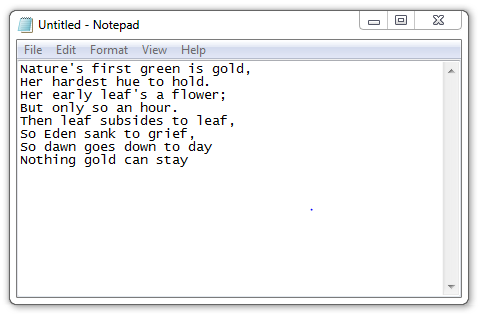
\includegraphics[width=0.85\textwidth]{Images/Chapter1/notepad.png}
        \caption{Notepad application for Windows 7.}
        \label{fig:ch1_notepad}
\end{figure}

A \acs{UI} that relies of visual cues, as the ones described above, is called a \ac{GUI}. The invention of such interfaces played a major role in the popularization of computers in the 80s. This is due to the fact that most users are more comfortable using such interfaces, as opposed to Command Line Interfaces (\acs{CLI}) that have been around since the late 60s.

In a \acs{CLI}, as opposed to an intuitive graphical interface, the user is presented with a \textbf{shell}\marginnotes{Shells are explained in Sections \ref{sec:ch1_terminology} and \ref{sec:ch1_sells}} prompt in which it can write commands to be interpreted by the \textbf{shell}. You can see an example below of a \acs{CLI} in which a user entered the command \textbf{\texttt{ls}} to list all files and folders in the working directory\marginnotes{In this book, the words \textbf{folder} and \textbf{directory} are used interchengeably}.

\begin{command_line}[Bash]
marcel@dell:~$ ls
Documents      Downloads      Pictures
Music          Video          seneca.pdf
marcel@dell:~$
\end{command_line}

In order to properly use a \acs{CLI}, the user needs to learn a series of commands that the shell understands, as well as the syntax of these commands. Hence, it should come to no surprise that most regular users prefer to use \acs{GUI}s which do not incur in such steep learning curves.

If you are reading this book, however, I expect you not to be a regular user. In fact, I expect you to be starting a career as systems analyst, a software developer, or other positions in the IT industry. For people like you, having a clear understanding of how to use a \acs{CLI} presents a number of advantages:
\begin{itemize}
    \item There are tasks that can only be achieved by using a \acs{CLI} because no \acs{GUI} has been created to perform them.
    \item Some tasks can be performed, using a \acs{CLI}, in a fraction of the time it would take using a \acs{GUI} tool.
    \item \acs{CLI}s can be accessed remotely in a fast and straightforward fashion, allowing you to control multiple systems from a single computer
    \item Users can quickly create scripts that run on \acs{CLI}s to automate repetitive tasks such as: adding new users to the system, backing up data, updating the system, etc.
    \item The steps required to perform some actions using \acs{GUI}s can vary a lot depending on which \acs{OS}, or Linux distribution, you are using. On the other hand, they are normally identical using a CLI. In fact, the same commands\marginnotes{With a few notable exceptions} can be used in all Linux distributions, Apple computers, and since 2016, even in Windows systems.
\end{itemize}

Most Linux distributions have a \acs{GUI} that allow regular users to achieve daily tasks such as web browsing, email, or writing documents. However, all Linux distributions also come with a terminal emulator that allow super users to do much more using a \acs{CLI}.

\section{Terminology}
\label{sec:ch1_terminology}

Before moving forward to learn how to use a Linux \acs{CLI}, It is important to notice the difference between three concepts that are often used interchangeably:

\begin{description}
\item[CLI] The \acs{CLI} is just the technical name of the method by which we interact with a computer by means of written instructions.
\item[Terminal] All major Linux distributions have a \acs{GUI}. However, they normally also provide you with a terminal, or more precisely a terminal emulator. A terminal emulator is nothing else than a program that provides us with a \acs{CLI} to interact with the \textbf{shell}.
\item[Shell] The \textbf{shell} is a software that reads keyboard commands and passes them to the \acs{OS} to carry out. Such commands could be used to perform simple tasks like listing the files in a particular folder, adding users to the system, creating folders, or complex tasks such as upgrading the \acs{OS}, installing applications, etc.
\end{description}


\section{Shells}
\label{sec:ch1_sells}

As mentioned before, a \textbf{shell} is a software that interprets commands passed by the user, and passes them to the \acs{OS}. However, just like there are multiple languages such as English, Spanish, or Mandarim, there are multiple shells available. Table~\ref{tab:ch1_shells} below presents a description of a few such shells\marginnotes{Many other shells exist, such as dash, ksh, etc}.

\begin{table}[!htbp]
   \myfloatalign
   \begin{tabularx}{\textwidth}{Xp{90mm}} \toprule
   %\tableheadline{Shell} & \tableheadline{Description}\\ \midrule
   \textbf{sh} & The Bourne shell, which has been distributed as the default \textbf{shell} for Unix since 1979. \\
   \textbf{bash} & Bourne Again Shell, an upgraded version of \textbf{sh}, written by the GNU Project, which has become the \textit{de facto} standard Linux shell. \\
   \textbf{csh} or \textbf{tcsh} & A Unix shell using a syntax similar to the \textbf{C} programming language. \textbf{tcsh} is identical to \textbf{csh}, with the addition of some extra features such as command-line completion.\\
   \bottomrule
   \end{tabularx}
\caption{Linux Shells}
\label{tab:ch1_shells}
\end{table}

In this book, we will cover exclusively the \textbf{bash shell}. This is due to the fact that \textbf{bash} is the default shell for the most widely used Linux distributions. In fact, it is hard to find a Linux distribution that does no come with a \textbf{bash shell}. That said, after learning how to use one shell, it is much easier to learn other shells, as they share many concepts and syntax.

\section*{Exercises}
\addcontentsline{toc}{section}{Exercises}

\begin{exercises}
   \item Explain, with your own words, what is a Command Line Interface (\acs{CLI}).
   \item Explain, with your own words, what is a Graphical User Interface (\acs{GUI}).
   \item What is the relationship between a terminal emulator, and a shell?
   \item Which commands are used to list all files in the working directory using the following shells: sh, bash, csh, dash, and ksh?
\end{exercises}

\chapter{Basic Shell Commands I}\label{ch:basic_commands}

In this chapter we will cover how to get access to a terminal emulator, as well as some very basic \textbf{bash} commands.

\section{Accessing a Terminal Emulator}

Once a user logs into a Linux \acs{OS} with a \acs{GUI}, there are multiple ways to get access to a \textbf{terminal emulator}. Some methods work only on a specific distribution, whereas some methods work on most distributions. In what follows, a list of methods to access terminal emulators are presented for some of the most popular desktop environments. The most commom Linux distribution for each desktop environment is presented in the margin notes.

\begin{description}
   \item[Gnome3] Press\marginpar{Debian, Red Hat, Fedora, CentOS, Kali} the super (windows) button to call the list of applications, and then type \textbf{\texttt{terminal}} in the search field, or search for the terminal in the provided applications list.
   \item[KDE] Click \marginpar{OpenSUSE, Kubuntu, Slackware} on the start button at the lower left, and then click on accessories, and finally on \textbf{\texttt{terminal}} .
   \item[Unity] Press\marginpar{Ubuntu} the super (windows) button to call the dash (or conversely click on the dash button at the upper left), and then type \textbf{\texttt{terminal}}.
\end{description}

In all of these desktop environments, the terminal emualtor can also be started by pressing \textbf{\texttt{crtl+alt+T}}.

\section{Terminal Basics}

Once the terminal emulator starts, the user is presented with an application displaying a blinking cursor at a \textbf{\texttt{shell prompt}}, just like shown bellow.

\begin{command_line}[Bash]
@@marcel@dell:~$@@
\end{command_line}

This prompt contain important information about the current parameters of the shell, namely: the username (\textbf{\texttt{marcel}}), system name (\textbf{\texttt{dell}}), and working directory (represented by a tilde [\textbf{\texttt{\texttildelow}}])\marginnotes{The \textbf{\texttt{\$}} separates command prompts from these current parameters}. A brief description of these parameters follows:

\begin{description}
\item [Username] Linux systems, as any Unix-like system, was designed to allow multiple users to access the system. When a terminal emulator starts, it assumes the user to be the same one that logged in into the GUI system. in Chapter \ref{ch:users_groups}, we will show how the \textbf{\texttt{su}} command can be used to switch users. In the example above, the username is \textbf{\texttt{marcel}}.

\item[System name] During the installation of Linux systems,  users are required to give your system (local machine) a name. When a terminal emulator starts, it assumes that you are using the local machine. In chapter XXX we will see how to log into remote machines using the \textbf{\texttt{ssh}} command. In the example above, my local machine is called is \textbf{\texttt{dell}}.

\item[Working directory] Imagine that you issue a command to create a file. In which directory will this file be created? The answer is: in the current \textbf{working directory}. When a terminal emulator starts, it assumes by default that you are at the home folder (directory) of the user currently logged in. Hence, whichever actions you perform will, by default, affect this directory. In Section \ref{sub:cd} , we will show how to use the \textbf{\texttt{cd}} command to change directories. In the example above, this home folder, which is located at \textbf{\texttt{/home/marcel}} is represented by a tilde (\textbf{\texttt{\texttildelow}}).
\end{description}

In what follows, a number of basic \textbf{\texttt{bash}}\marginnotes{You can easily switch shells by typing the name of the shell you want to switch to. For example, you can type \textbf{\texttt{dash}} to start using a \textbf{dash shell}} commands are presented.

\section{\textbf{\texttt{date}}}
To ask what day is today, you can type \textbf{\texttt{date}} \index{date} in the terminal emulator and press enter. The shell will verify the date with the \acs{OS}, display it in the terminal, and start a new prompt line ready to receive more commands, as shown below\marginnotes{For the following commands, we will ommit this new prompt line}. Note that the terminal also shows the current time and the time zone (Eastern Daylight Time - EDT).

\begin{command_line}[Bash]
@@marcel@dell:~$@@ date
Wed May 18 19:20:55 EDT 2016
@@marcel@dell:~$@@
\end{command_line}

Note that shell commands are \textbf{case-sensitive}. I.e., the shell diferentiates between upper-case and lower-case letters. For example, while \textbf{\texttt{date}} is a valid command, \textbf{\texttt{Date}} and \textbf{\texttt{DATE}} are not.

\section{\textbf{\texttt{whoami}}}
Not all terminal emulators display the username at each command prompt. Therefore, the shell needs to provide a method to verify the username of the current user. This is accomplished by the \textbf{\texttt{whoami}} (who am I) command, as shown below.

\begin{command_line}[Bash]
@@marcel@dell:~$@@ whoami
marcel
\end{command_line}

\section{\textbf{\texttt{pwd}}}
%The concept of a hyerarchical filesystem in which users can have create folders (directories) inside other folders was introduced with Unix. This concept is used by most modern OS, and Linux is no exception to this rule.

As mentioned before, when a terminal emulator is open, it needs a directory to act as a starting point. In most Linux system, this starting point is the user's home folder, located at \textbf{\texttt{/home/username}}, represented by a tilde (\textbf{\texttt{\texttildelow}}).

As we will show later, users can move to different directories using the shell. The shell's current location is called \textbf{working directory}. This is due to the fact that this is the directory that the shell will, by default, act (work) upon. In order to see in which directory you are currently at, you can type \textbf{\texttt{pwd}}\marginnotes{short for print working directory} in the terminal emulator and press enter. The shell will then print the working directory in the terminal, as shown below.

\begin{command_line}[C]
@@marcel@dell:~$@@ pwd
/home/marcel
\end{command_line}

\section{\textbf{\texttt{ls}}}
\label{sec:ls}

To obtain a list of all files and folders present in the working directory, as demonstrated in Chapter \ref{ch:cli_terminal_shell}, you can use the \textbf{\texttt{ls}}\marginnotes{short for list} command. The shell will then print a list of all files and folders, as shown below\marginnotes{Some terminal emulators use colours to distinguish between files, folders, scripts, etc}.

\begin{command_line}[Bash]
@@marcel@dell:~$@@ ls
Documents      Downloads      Pictures
Music          Video          seneca.pdf
\end{command_line}

The list command, by default, does not show hidden files\marginnotes{Hidden files are files whose names starts with a \textbf{\texttt{.}} (dot)}. In order to do so, you must add the option \textbf{\texttt{-a}} or \textbf{\texttt{--all}} to the ls command, as shown below:
\begin{command_line}[Bash]
@@marcel@dell:~$@@ ls
Documents      Downloads      Pictures
Music          Video          seneca.pdf
@@marcel@dell:~$@@ ls -a
.              ..             Documents
Downloads      Pictures       Music
Video          seneca.pdf     .System.conf
\end{command_line}
Note that in the command above, the file \textbf{\texttt{.System.conf}} only appears when the \textbf{\texttt{ls}} command is issued with the \textbf{\texttt{-a}} option. Also, note that two extra directories appear: a folder (\textbf{\texttt{.}}) and a folder (\textbf{\texttt{..}}). These are not real directories. They are simply hard links to the self (\textbf{\texttt{.}}) and parent (\textbf{\texttt{..}}) directories.

The list comand can also used to gather information about the files and folders in the current working directory. To do so, the \textbf{long list} option \textbf{\texttt{-l}} must be invoked, as shown below:
\begin{command_line}[Bash]
@@marcel@dell:~$@@ ls -a -l
drwxrwxr-x  3 marcel marcel  4096 Jun 21 23:06 .
drwxr-xr-x 54 marcel marcel  4096 Jun 21 18:59 ..
drwxrwxr-x  2 marcel marcel  4096 Jun 21 23:06 Documents
drwxrwxr-x  2 marcel marcel  4096 Jun 21 23:06 Downloads
drwxrwxr-x  2 marcel marcel  4096 Jun 21 23:06 Pictures
drwxrwxr-x  2 marcel marcel  4096 Jun 21 23:06 Music
drwxrwxr-x  2 marcel marcel  4096 Jun 21 23:06 Video
-rw-rw-r--  1 marcel marcel 12238 Jun 29 22:54 seneca.pdf
-rw-rw-r--  1 marcel marcel   126 Jun 28 20:52 .System.conf
\end{command_line}
This long list provides a number fo columns containing information about each file. In Table~ \ref{tab:ch2_list}, we explain what the information in each column represents using the file \textbf{\texttt{seneca.pdf}} as an example.

\begin{table}[!htbp]
   \myfloatalign
   \begin{tabularx}{\textwidth}{cXp{70mm}} \toprule
   %\tableheadline{Shell} & \tableheadline{Description}\\ \midrule
   \textbf{column} & \textbf{example} & \textbf{meaning} \\ \bottomrule
   \textbf{1} & \textbf{\texttt{-rw-rw-r--}} & File type and permission sets. These topics are covered in Chapter \ref{ch:users_groups}.\\
   \textbf{2} & \textbf{1} & Number of hard links to this file. Links are covered in Chapter \ref{ch:file_links}.\\
   \textbf{3} & \textbf{marcel} & Name of the user owner of the file. The concepts of users and ownership are covered in Chapter \ref{ch:users_groups}.\\
   \textbf{4} & \textbf{marcel} & Name of the group owner of the file. The concepts of groups and ownership are covered in Chapter \ref{ch:users_groups}.\\
   \textbf{5} & \textbf{12238} & Size of the file in bytes.\\
   \textbf{6} & \textbf{Jun 29 22:54} & Timestamp indicating when the file was edited for the last time.\\
   \textbf{7} & \textbf{seneca.pdf} & File name.\\
   \bottomrule
   \end{tabularx}
\caption{Long list information for the \textbf{\texttt{seneca.pdf}} file.}
\label{tab:ch2_list}
\end{table}

\section{\textbf{\texttt{tree}}}
The \mycommand{tree} command is somewhat similar to the \mycommand{ls} command. They both display a list of files and folders in the working directory. However, contrary to \mycommand{ls}, in which any subfolder is simply listed alongside files, the \mycommand{tree} command goes inside each subfolder and displays the files contained in them, creating a tree-like structure. See the example below:
\begin{command_line}
@@marcel@dell:Seneca$@@tree
.
|-- academic_honesty.pdf
|-- calendar.pdf
|-- OPS105
|   |-- students_list
|   |-- grades.xls
|-- SRT311
|   |-- students_list
|   |-- grades.xls

2 directories, 6 files
@@marcel@dell:Seneca$@@
\end{command_line}

The \mycommand{tree} command is not available by default in some Linux distributions. To install it, you must write the command \mycommand{sudo apt-get install tree}, and enter your user password.

\section{\textbf{\texttt{cd}}}
\label{sub:cd}
To switch working directories, you need only to use the \textbf{\texttt{cd}}\marginnotes{short for change directory} command, followed by the name of the directory you want to go. For example, assuming that the folders shown in the previous command's output do exist, typing \textbf{\texttt{cd Documents}} results in:
\begin{command_line}
@@marcel@dell:~$@@ pwd
/home/marcel
@@marcel@dell:~$@@ cd Documents
@@marcel@dell:Documents$@@ pwd
/home/marcel/Documents
\end{command_line}

The command \textbf{\texttt{cd}} by itself always sends the user back to the user's home folder. Also, the command \textbf{\texttt{cd ..}} sends the user to the parent folder of the working directory, and the command \textbf{\texttt{cd -}} sends the user back to the previous working directory. The parent folder is the folder hierarchically above the current folder. For example, the folder \textbf{\texttt{/home/marcel}} is the parent folder of \textbf{\texttt{/home/marcel/Documents}}.

Finally, note that if you enter the name of a directory that does not exist, the shell will return an error message and then it will start a new prompt line ready to receive more commands, as shown next.

\begin{command_line}[make]
@@marcel@dell:~$@@ cd DOCUMENTS
bash: cd: DOCUMENTS: No such file or directory
@@marcel@dell:~$@@
\end{command_line}

\section{Relative and Absolute Paths}

In our previous example using the \textbf{\texttt{cd}} command, we switched working directories from one folder, \textbf{\texttt{/home/marcel}}, to one of its immediate subfolders, \textbf{\texttt{/home/marcel/Documents}}. However, you might face more complex situations in which you have a directory tree as shown in Figure \ref{fig:ch2_dirtree}, and you want to switch the current working directory from any folder directly to any other folder.

\begin{figure}[!htbp]
  \centering
        \tikzstyle{every node}=[thick,anchor=west, font={\scriptsize\ttfamily}, inner sep=2.5pt]
\tikzstyle{selected}=[draw=black]
\tikzstyle{root}=[selected, fill=black!20]

\begin{tikzpicture}[%
    scale=.99,
    grow via three points={one child at (0.5,-0.65) and
    two children at (0.5,-0.65) and (0.5,-1.1)},
    edge from parent path={(\tikzparentnode.south) |- (\tikzchildnode.west)}]
  \node [root] {/}
    child { node [selected] {home}
      child { node [selected] {marcel}
        child { node [selected] {Seneca}
           child { node {ops105.sh}}
           child { node {srt311.py}}
        }
        child { node at (0, -2.0) [selected] {Personal}
           child { node {bills.doc}}
           child { node {summer.jpg}}
        }
      }
    }
    child { node at (0,-5.0) [selected] {media}
      child { node [selected] {Seneca}
        child { node {bts490.c}}
        child { node {btn415.cpp}}
      }
    }
    child { node at (0,-7.0) {\dots}};
\end{tikzpicture}

        \caption{Directory tree.}
        \label{fig:ch2_dirtree}
\end{figure}

For example, given the directory tree shown in Figure \ref{fig:ch2_dirtree}, how can we directly switch working directories for the following cases:
\begin{itemize}
\item from \textbf{\texttt{/home}} directly to \textbf{\texttt{/home/marcel/Personal}}
\item from \textbf{\texttt{/home/marcel/Seneca}} directly to \textbf{\texttt{/media}}
\item from \textbf{\texttt{/home/marcel/Seneca}} to \textbf{\texttt{/media/Seneca}}
\end{itemize}
The solution to all these cases is: ``by providing either a \textbf{relative path} or an \textbf{absolute path} to the desired folders.'' In what follows, we define these two concepts\marginnotes{Note that the concepts of relative and absolute paths also apply to files}.

\subsection{Relative Path}
 When a relative path is provided, the shell assumes that the starting point of the path is the current working directory. For example, given that you are currently in \textbf{\texttt{/home}}, you can switch your working directory to \textbf{\texttt{/home/marcel/Personal}} by issuing the command: \textbf{\texttt{cd marcel/Personal}}, as shown in what follows.
\begin{command_line}
@@marcel@dell:home$@@ pwd
/home
@@marcel@dell:home$@@ cd marcel/Personal
@@marcel@dell:Personal$@@ pwd
/home/marcel/Personal
\end{command_line}
\subsection{Absolute Path}
 Absolute paths always start with \textbf{\texttt{/}}\marginnotes{\textbf{\texttt{/}} denotes the root, of all directories in a Linux system} and provide the complete path for the desired folder or file. For example, given that your working directory is \textbf{\texttt{/home/marcel/Seneca}}, you can switch to \textbf{\texttt{/media}} by issuing the command: \textbf{\texttt{cd /media}}, or you can switch  to \textbf{\texttt{/media/Seneca}} by issuing the command: \textbf{\texttt{cd /media/Seneca}} , as shown in what follows.
\begin{command_line}
@@marcel@dell:Seneca$@@ pwd
/home/marcel/Seneca
@@marcel@dell:Seneca$@@ cd /media
@@marcel@dell:media$@@ pwd
/media
\end{command_line}
\begin{command_line}
@@marcel@dell:Seneca$@@ pwd
/home/marcel/Seneca
@@marcel@dell:Seneca$@@ cd /media/Seneca
@@marcel@dell:Seneca$@@ pwd
/media/Seneca
\end{command_line}

Relative and absolute paths can be compared to addresses in navigation systems. For example, if you live in Toronto, and you want to go to a place within the city, you can type on your navigation device an address such as 200 King Street. The device will assume that this address is in Toronto-ON, Canada. This would be the compared to a relative address, as the starting point is assumed to be the city of Toronto. However, if you are in Toronto and you want to go to 200 King Street in Buffalo-NY, you would need to enter the complete address, including the city, state, and sometimes even the country. This would be compared to an absolute value, as the address is completely defined.

\section{\textbf{\texttt{clear}}}

All commands you enter, as well as their outputs, stay in the screen and you are given a new shell prompt at the bottom to keep working with the shell. This can lead to a very polluted screen containing a lot of information that is no longer necessary.

In order to clear the screen from all previous commands and ouputs, you simple have to issue the \textbf{\texttt{clear}} command. This command will erase from your terminal all information in it and provide you with a command prompt at the top to keep working with the shell.

It is important to note that this command simply clears the terminal display. Any variables\marginnotes{Variables are covered in Chapter~\ref{ch:intro_scripting}} that have been defined, or any modifications to the state of the shell will not be changed by this command.

\section{Command History}

You can use the up ($\uparrow$) and down ($\downarrow$) arrow keys in order to navigate the commands you have previously entered in your shell. For example, by hitting the up arrow key once, you will get the previously entered command. Hitting the up arrow again, will get you the command you entered prior to that one.

\section*{Exercises}
\addcontentsline{toc}{section}{Exercises}

\begin{exercises}
   \item Describe two methods to open a terminal emulator on a Ubuntu Linux OS.
   \item Given the command prompt below, who is the user currently logged into the shell? Also, what is the name of the local machine? Finally, what is the current working directory?
\begin{command_line}
@@john@lenovo:~$@@
\end{command_line}
   \item What is the relationship between a \textbf{terminal emulator}, and a \textbf{shell}?
   \item Which commands are used to list all files in the working directory using the following shells: bash, csh, dash, and ksh?
   \item Which command can be used to show in the terminal what time is it?
   \item What is the output of the \textbf{\texttt{ls -l}} command? What does the 6$^{\text{th}}$ column represents?
   \item How can you move back to the latest previously accessed working directory using only one shell command?
   \item What happens when you apply the parent folder parameter to the \textbf{\texttt{cd}} command twice. In other words, what happens when you issue a \textbf{\texttt{cd ../..}} command?

Given the directory tree shown in Figure \ref{fig:ch2_ex_dirtree} (on next page), answer the following questions:
\begin{figure}[!htbp]
  \centering
        \tikzstyle{every node}=[thick,anchor=west, font={\scriptsize\ttfamily}, inner sep=2.5pt]
\tikzstyle{selected}=[draw=black]
\tikzstyle{root}=[selected, fill=black!20]

\begin{tikzpicture}[%
    scale=.99,
    grow via three points={one child at (0.5,-0.65) and
    two children at (0.5,-0.65) and (0.5,-1.1)},
    edge from parent path={(\tikzparentnode.south) |- (\tikzchildnode.west)}]
  \node [root] {/}
    child { node [selected] {home}
      child { node [selected] {marcel}
          child { node {ops105.sh}}
          child { node {srt311.py}}
        }
      }
    child { node at (0,-2.0) [selected] {media}
      child { node [selected] {Seneca}
        child { node {bts490.c}}
        child { node {btn415.cpp}}
      }
    }
    child { node at (0,-4.0) {\dots}};
\end{tikzpicture}

        \caption{Directory tree for questions 9, 10, and 11.}
        \label{fig:ch2_ex_dirtree}
\end{figure}
   \item Write a command to switch your working directory from \textbf{marcel} to \textbf{Seneca} using only one shell command?
   \item Write a command to switch your working directory from \textbf{media} to \textbf{marcel} using only one shell command.
   \item Given that your working directory is \textbf{media}, can you use a relative path to move to \textbf{Seneca}? If yes, can you also use an absolute path? Which one of these options seem more appropriate in this case?
\end{exercises}

\chapter{Basic Shell Commands II}\label{ch:basic_commands_ii}

In our previous chapter, we covered a number of bash commands which could be used to: gather information from the system and user (\textbf{\texttt{date}},  \textbf{\texttt{whoami}}, \textbf{\texttt{pwd}}), get information about files and folders (\textbf{\texttt{ls}}), or to change de current working directory (\textbf{\texttt{cd}}).

None of the commands could be used to alter files, folders, or change the configurations of the system, though. I.e., they have no lasting effect in the system.

In this chapter, we will cover a series of commands that have lasting effects in files, folders, and possibly the system. The commands we are covering in this chapter can be used to create and remove files and folders, as well as to rename and make copies of them.

\section{\textbf{\texttt{mkdir}}}

To create new folders, the \textbf{\texttt{mkdir}}\marginnotes{short for make directory} command can be used, followed by the name(s) of the folder(s) to be created. In the example below, a folder called \textbf{Samples} is created in the current working directory.

\begin{command_line}[Bash]
@@marcel@dell:~$@@ ls
Documents      Downloads      Pictures
Music          Video          seneca.pdf
@@marcel@dell:~$@@ mkdir Samples
@@marcel@dell:~$@@ ls
Documents      Downloads      Pictures    @@Samples@@
Music          Video          seneca.pdf
\end{command_line}

Note that, by default, the new directory is created as a subfolder of the working directory. To create folders in other locations, without leaving the current working directory, you can use the \textbf{\texttt{mkdir}} command combined with relative or absolute paths, as shown below:

\begin{command_line}[Bash]
@@marcel@dell:~$@@ ls Documents
Seneca      Personal
@@marcel@dell:~$@@ mkdir ~/Documents/Samples
@@marcel@dell:~$@@ ls Documents
Seneca      Personal    @@Samples@@
\end{command_line}

\begin{my_box}[Files and Folders with spaces in their names]
  In all examples that were given so far is this book, all files and folders do not contain spaces in their names. Issuing a command such as \textbf{\texttt{mkdir My Documents}} would create two folders, one called \textbf{\texttt{My}} and another called \textbf{\texttt{Documents}}. This is because the shell cannot distinguish between an argument with a space, or two arguments without spaces.

  Linux can handle files and folder with spaces, though. In order to do so, whenever you are refering to a file or folder with sapces in its name, each space needs to be preceeded by a backslash (\textbf{\texttt{\textbackslash}}). For example, you can create a folder called \textbf{\texttt{My Documents}} by issuing a command \textbf{\texttt{mkdir My\textbackslash Documents}}.
\end{my_box}


\section{\textbf{\texttt{rmdir}}}

The \textbf{\texttt{rmdir}}\marginnotes{short for remove directory} command, as the name suggests, deletes existing folders. For example, \textbf{\texttt{rmdir Samples}} will remove a folder \textbf{\texttt{Samples}} from the current working directory. It is important to note that it can only be used to remove empty folders. In case the folder is not empty, the shell returns an error message.

In the example below, the \textbf{\texttt{rmdir}} command is applied to both an empty folder \textbf{Samples}, and to a non-empty folder \textbf{Pictures}.
\begin{command_line}[Bash]
@@marcel@dell:~$@@ ls
Documents      Downloads      Pictures    @@Samples@@
Music          Video          seneca.pdf
@@marcel@dell:~$@@ rmdir Samples
@@marcel@dell:~$@@ ls
Documents      Downloads      Pictures    Music
Video          seneca.pdf
@@marcel@dell:~$@@ rmdir Pictures
rmdir: failed to remove 'Pictures': Directory not empty
@@marcel@dell:~$@@
\end{command_line}

\section{\textbf{\texttt{touch}}}

As shown in Section \ref{sec:ls}, files and folders in Linux have a timestamp indicating when they were edited for the last time. The \textbf{\texttt{touch}} command, when applied to an existing file, updates the timestamp of when it was last edited\marginnotes{Updated timestamps are useful for some backup programs, among other uses}. It is equivalent to opening the file, saving it, and then closing it. As an example, see the command prompt below:
\begin{command_line}[Bash]
@@marcel@dell:~$@@ ls -l
total 0
-rw-rw-r-- 1 marcel marcel 0 Jul 12 11:31 final_exam.doc
-rw-rw-r-- 1 marcel marcel 0 Jun 21 20:30 introduction.ppt
-rw-rw-r-- 1 marcel marcel 0 May 10 21:41 seneca.pdf
@@marcel@dell:~$@@ touch final_exam.doc
@@marcel@dell:~$@@ ls -l
total 0
-rw-rw-r-- 1 marcel marcel 0 @@Jul 14 22:12@@ final_exam.doc
-rw-rw-r-- 1 marcel marcel 0 Jun 21 20:30 introduction.ppt
-rw-rw-r-- 1 marcel marcel 0 May 10 21:41 seneca.pdf
\end{command_line}
When applied to non-existing files, the \textbf{\texttt{touch}} command creates empty files, as shown below:
\begin{command_line}[Bash]
@@marcel@dell:~$@@ ls -l
total 0
-rw-rw-r-- 1 marcel marcel 0 Jul 14 22:12 final_exam.doc
-rw-rw-r-- 1 marcel marcel 0 Jun 21 20:30 introduction.ppt
-rw-rw-r-- 1 marcel marcel 0 May 10 21:41 seneca.pdf
@@marcel@dell:~$@@ touch mid_term.doc
@@marcel@dell:~$@@ ls -l
total 0
-rw-rw-r-- 1 marcel marcel 0 Jul 14 22:12 final_exam.doc
-rw-rw-r-- 1 marcel marcel 0 Jun 21 20:30 introduction.ppt
-rw-rw-r-- 1 marcel marcel 0 May 10 21:41 seneca.pdf
@@-rw-rw-r-- 1 marcel marcel 0 Jul 14 22:15 mid_term.doc@@
\end{command_line}
This second usage of the \textbf{\texttt{touch}} command is frequently used for testing purposes\marginnotes{tip: you to use \textbf{\texttt{touch}} and \textbf{\texttt{mkdir}} in order to recreate the examples provided in this chapter.}.

\section{\textbf{\texttt{rm}}}

To delete (remove) files, the \textbf{\texttt{rm}}\marginnotes{short for remove} command can be used, followed by the name(s) of file(s) to be deleted from the working directory. See the example below:

\begin{command_line}[Bash]
@@marcel@dell:~$@@ ls
Documents      Downloads      Pictures
Music          Video          @@seneca.pdf@@
@@marcel@dell:~$@@ rm seneca.pdf
@@marcel@dell:~$@@ ls
Documents      Downloads      Pictures
Music          Video
\end{command_line}

The \textbf{\texttt{rm}} command can also be used to remove non-empty folders. To do so, we have to apply the \textbf{\texttt{-r}} (recursive) option followed by the name of the folder, as shown below.
\begin{command_line}[Bash]
@@marcel@dell:~$@@ ls
Documents      Downloads      @@Pictures@@
Music          Video          seneca.pdf
@@marcel@dell:~$@@ rm -r Pictures
@@marcel@dell:~$@@ ls
Documents      Downloads      Music
Video          seneca.pdf
\end{command_line}

%It is important to note that, by default, this command does not ask for confirmation, prior to deleting the file. Also, most Linux distributions do not have a recycle being. Hence, it is important to be careful before using this command.

\begin{my_box}[Bash Design Goals]
  It is important to note that the commands described in this chapter don't normally ask for confirmation. For example, when deleting a file using the \textbf{\texttt{rm}} command, the \textbf{shell} will not ask the user if he/she is sure he/she wants to delete the file. Nor the file will be sent to a recycle bin from which it can be recovered. The file will simply be deleted.

  The \textbf{shell} performs tasks that might incur in unforeseen consequences, such as accidently deleting a number of files, in a much more direct way because of its design goals. As opposed to \acs{GUI} interfaces where the goal normally is to provide a platform for inexperienced users to perform basic tasks, a \acs{CLI} is normally designed with the goal of allowing experienced users to quickly perform complex tasks.
\end{my_box}

\section{\textbf{\texttt{mv}}}

The \textbf{\texttt{mv}}\marginnotes{short for move} command can be used in two distinct ways. As the name suggests, it can move a file, a folder, or a number of files and folders from one directory to another. However, it can also be used to rename single files or folders. Both uses of this command are described in what follows.

\subsection{Moving files and folders accross directories}

To move a single file from one directory to another, the \textbf{\texttt{mv}} command needs two arguments. The first being the name of the file in the working directory to be moved, and the second being the absolute or relative path of the directory we are moving the file to. See the example below:
\begin{command_line}[Bash]
@@marcel@dell:~$@@ ls
@@final_exam.doc@@  introduction.ppt  seneca.pdf
Folder
@@marcel@dell:~$@@ mv final_exam.doc Folder
@@marcel@dell:~$@@ ls
introduction.ppt  seneca.pdf  Folder
@@marcel@dell:~$@@ ls Folder
@@final_exam.doc@@
@@marcel@dell:~$@@
\end{command_line}

Note that, in this example, the file \textbf{final\_exam.doc} disappears from the working directory and appears in the \textbf{Folder} directory.

Multiple files can be moved with a single \textbf{\texttt{mv}} command. To do so, you first need to provide the names of all files you intend to move as arguments. Then, you need to provide the relative or absolute path of the directory you want to move them to as the very last argument. This technique is  shown in what follows:
\begin{command_line}[Bash]
@@marcel@dell:~$@@ ls
@@final_exam.doc@@  @@introduction.ppt@@  seneca.pdf
Folder
@@marcel@dell:~$@@ mv final_exam.doc introduction.ppt Folder
@@marcel@dell:~$@@ ls
seneca.pdf  Folder
@@marcel@dell:~$@@ ls Folder
@@final_exam.doc@@ @@introduction.ppt@@
@@marcel@dell:~$@@
\end{command_line}

Note that, within this context, this command can also be applied to folders (directories). I.e., you can move an entire folder in your working directory into other folders using the exactly same syntax applied for files in this section.

\subsection{Renaming files and folders}

Imagine the \textbf{\texttt{mv}} command being used with two arguments, the first being a file name in the working directory, and the second being a name that doesn't match any directories. In this scenario, the \textbf{\texttt{mv}} command will rename the file indicated by the first argument to the name specified in the second\marginnotes{A command called \textbf{\texttt{rename}} exists in \textbf{\texttt{bash}}. However, it is used to rename multiple files at once using regular expressions. Regular expressions are covered in Chapter~\ref{ch:grep}}. See the example below:
\begin{command_line}[Bash]
@@marcel@dell:~$@@ ls
@@final_exam.doc@@  introduction.ppt  seneca.pdf
Folder
@@marcel@dell:~$@@ mv final_exam.doc final_exam_fall.doc
@@marcel@dell:~$@@ ls
@@final_exam_fall.doc@@  introduction.ppt  seneca.pdf
Folder
@@marcel@dell:~$@@
\end{command_line}
In this example, you can see that the file \textbf{final\_exam.doc} was renamed to \textbf{final\_exam\_fall.doc}.

You can also rename a folder using the same syntax applied for files in this section.

\section{\textbf{\texttt{cp}}}

The \textbf{\texttt{cp}}\marginnotes{short for copy} command can be used to copy files and folders. It can be used in two distinct ways:


\subsection{Copying files within the working directory}

To create a copy of a file in the same working direct, the \textbf{\texttt{cp}} command should be used with two arguments. The first argument should be the name of the file to be copied, while the second argument should be the name of the copy, as shown below:
\begin{command_line}[Bash]
@@marcel@dell:~$@@ ls
final_exam.doc  introduction.ppt  seneca.pdf
Folder
@@marcel@dell:~$@@ cp final_exam.doc final_exam_fall.doc
@@marcel@dell:~$@@ ls
final_exam.doc  @@final_exam_fall.doc@@  introduction.ppt
seneca.pdf  Folder
@@marcel@dell:~$@@
\end{command_line}

To copy an entire folder in your working directory into another folder also in the working directory, you must use the recursive option \textbf{\texttt{-r}}, as shown in the example below:
\begin{command_line}[Bash]
@@marcel@dell:~$@@ ls
final_exam.doc  introduction.ppt  seneca.pdf
Folder
@@marcel@dell:~$@@ cp -r Folder Folder_Copy
@@marcel@dell:~$@@ ls
final_exam.doc  final_exam_fall.doc  introduction.ppt
seneca.pdf  Folder  @@Folder_Copy@@
@@marcel@dell:~$@@
\end{command_line}

\subsection{Copying files to other directories}

To create a copy of a file in the working directory to another directory, the second argument of the \textbf{\texttt{cp}} command must be the absolute or relative path of the directory in which you want to plae a copy of the file. In this case, the new file will have the same name as the original file. See the example below:
\begin{command_line}[Bash]
@@marcel@dell:~$@@ ls
final_exam.doc  introduction.ppt  seneca.pdf
Folder
@@marcel@dell:~$@@ cp final_exam.doc Folder
@@marcel@dell:~$@@ ls
final_exam.doc  introduction.ppt  seneca.pdf
@@Folder@@
@@marcel@dell:~$@@ ls Folder
@@marcel@dell:~$@@ ls
final_exam.doc
@@marcel@dell:~$@@
\end{command_line}

Just as with the previous scenario, to copy an entire folder in the working directory to another directory, you also must use the recursive option \textbf{\texttt{-r}}. See the example below:
\begin{command_line}[Bash]
@@marcel@dell:~$@@ ls
final_exam.doc  introduction.ppt  seneca.pdf
Folder  Music
@@marcel@dell:~$@@ cp Music Folder
cp: omitting directory 'Music'
@@marcel@dell:~$@@ ls Folder
final_exam.doc  introduction.ppt
@@marcel@dell:~$@@ cp -r Music Folder
@@marcel@dell:~$@@ ls Folder
final_exam.doc  introduction.ppt  @@Music@@
@@marcel@dell:~$@@
\end{command_line}

To copy all contents of a folder to another folder, but not the folder itself, you need to add \textbf{\texttt{/.}} to the end of the name of the folder you are copying, as shown below\marginnotes{You can also use this technique with the \textbf{\texttt{mv}} command}:
\begin{command_line}[Bash]
@@marcel@dell:~$@@ ls
final_exam.doc  introduction.ppt  seneca.pdf
Folder  Music
@@marcel@dell:~$@@ cp -r Music/. Folder
@@marcel@dell:~$@@ ls Folder
arcade_fire-ready_to_start.mp3  foo_fighters-walk.mp3
@@marcel@dell:~$@@
\end{command_line}


\section*{Exercises}
\addcontentsline{toc}{section}{Exercises}

\begin{exercises}
   \item What is the main difference between using the copy \textbf{\texttt{cp}}, and the move \textbf{\texttt{mv}} commands, when applied to files?
   \item How can you delete a non-empty folder called \textbf{Archive} that exists in your working directory?
   \item Which command can be used to move a file called \textbf{README.txt} from your working directory to its parent folder
   \item Which command can be used to create a folder called \textbf{Examples} inside a subfolder called \textbf{Documentation} that exists in your working directory. See the diagram in Figure \ref{fig:ch3_dirtree}.
   \begin{figure}[!htbp]
     \centering
           \tikzstyle{every node}=[thick,anchor=west, font={\scriptsize\ttfamily}, inner sep=2.5pt]
\tikzstyle{selected}=[draw=black]
\tikzstyle{created}=[draw=gray,dashed]
\tikzstyle{root}=[selected, fill=black!20]

\begin{tikzpicture}[%
    scale=.99,
    grow via three points={one child at (0.5,-0.65) and
    two children at (0.5,-0.65) and (0.5,-1.1)},
    edge from parent path={(\tikzparentnode.south) |- (\tikzchildnode.west)}]
  \node [root] {/}
    child { node [selected] {home}
      child { node [selected] {marcel}
        child { node [selected] {Documentation}
           child { node [created] {Examples}}
           child { node {Example1.txt}}
           child { node {Example2.txt}}
        }
        child { node at (0, -2.0) [selected] {Personal}
           child { node {bills.doc}}
           child { node {summer.jpg}}
        }
      }
    }
    child { node at (0,-5.0) {\dots}};
\end{tikzpicture}

           \caption{Directory tree for questions 4 and 5.}
           \label{fig:ch3_dirtree}
   \end{figure}
   \item Still with regards to the diagram diagram in Figure \ref{fig:ch3_dirtree}, how can you move files \textbf{Example1.txt} and \textbf{Example2.txt} from the \textbf{Documentation} folder to its \textbf{Examples} subfolder, without changing your working directory.
   \item Is it possible to delete multiple empty folders with only one \textbf{\texttt{rmdir}} command? If so, how can you delete two empty folders named \textbf{Tests} and \textbf{Assignments} from your working directory?
   \item What happens when you apply the \textbf{\texttt{touch}} command to an existing file? Also, what happens when you apply this command to a non-existing file.
   \item How can you make copies of the contents of a file called \textbf{exams.txt} from your working directory, to a file called \textbf{exams.txt} inside a subfolder \textbf{Classes} that exists in your working directory?
   \item What happens when the first parameter of a \textbf{\texttt{mv}} command is a file, and the second parameter is a folder?
   \item Which command can be used to copy the contents of a subfolder named \textbf{Folder1}, that exists in the current working directory, to another subfolder named  \textbf{Folder1Copy} in the same working directory. Note that the subfolder \textbf{Folder1Copy} doesn't exist prior to the command you need to enter.
\end{exercises}

%************************************************
\chapter{Getting Help}\label{ch:getting_help}
%************************************************
We have already covered in previous chapters a number of commands which can take multiple options and different numbers of arguments. For example, it was shown in Chapter \ref{ch:basic_commands} that the command \textbf{\texttt{ls}} can work in three different ways:

\begin{itemize}
  \item By itself, this command prints the names of all files in the working directory.
  \item When provided with the name of another folder as an argument, this command prints the names of all files in the specified folder.
  \item If called with the the option \textbf{\texttt{-l}}\marginnotes{There are many more options for the \textbf{\texttt{ls}} command.}, this command gives all the information about files described on Table \ref{tab:ch2_list}, as opposed to just listing their names.
\end{itemize}

The bash shell has hundreds of commands like \textbf{\texttt{ls}} that can take multiple options and different numbers of arguments. Hence, in order to be accessible to non-experts, it needs to provide its users with a way of knowing how to use those commands.

In this chapter we will cover different ways in which users can get help on how to use different commands.

\section{\textbf{\texttt{help}}}

By itself, the \textbf{\texttt{help}} command will list all \textbf{built-in}\marginnotes{Built-in commands are explained in the Built-in Commands box that follows} commands. If one of the built-in commands is provided as an argument, this command provides a quick description of the provided command, and possibly a list of options. You can see below the output of entering \textbf{\texttt{help pwd}} on bash.

\begin{command_line}[make]
@@marcel@dell:~$@@ help pwd
pwd: pwd [-LP]
    Print the name of the current working directory.

    Options:
      -L	print the value of $PWD if it names the current working directory
      -P	print the physical directory, without any symbolic links

    By default, 'pwd' behaves as if '-L' were specified.

    Exit Status:
    Returns 0 unless an invalid option is given or the current directory cannot be read.\end{command_line}

Note that \textbf{\texttt{help}} only covers built-in commands. It does not cover commands implemented as binary files in \textbf{/bin} or \textbf{/usr/bin}, such as \textbf{\texttt{ls}}, \textbf{\texttt{rm}}, \textbf{\texttt{mv}}, and many others.


\begin{my_box}[Built-in Commands]
  Most commands in bash, such as \textbf{\texttt{ls}}, \textbf{\texttt{rm}}, and \textbf{\texttt{touch}} are implemented by binary files located in the \textbf{/bin} and \textbf{/usr/bin} folders. These commands are interpreted in the same way as any other application the shell can run. I.e., the shell asks the kernel to execute it, and after it has finished executing, the shell receives its output.

  Built-in commands, on the other hand, are an integral part of the shell. They are not implemented in a separated file. The main reason why some commands are implemented directly inside the shell is because they need to change the state of the shell. For example, the \textbf{\texttt{cd}} command is a built-in command because it changes the current working directory. Commands implemented as binaries, such as \textbf{\texttt{ls}}, \textbf{\texttt{rm}}, and \textbf{\texttt{touch}}, cannot change the state of the shell.

  Another reason for implementing some commands directly into the shell is because it normally enhances their performance.
\end{my_box}

\section{\textbf{\texttt{man}}}

Since the inception of Unix, it has become standard practice for the authors of scripts that implement shell commands to provide manual pages for them. This practice was continued by the GNU project when rewritting Unix as an open source project\marginnotes{In fact, the author of the manual pages for many basic commands such as \textbf{\texttt{ls}} and \textbf{\texttt{rm}} is no one less than Richard Stallman, the programmer that started the GNU project, as discussed in Chapter~\ref{ch:history}}.

All manual pages follow the same structure show in Listing \ref{lst:mkdir_man} (page \pageref{lst:mkdir_man}). I.e., they have the following sections:

\begin{source_code_float}{make}{Manual page for the \textbf{\texttt{mkdir}} command.}{lst:mkdir_man}
  MKDIR(1)            User Commands               MKDIR(1)

  NAME
         mkdir - make directories
  SYNOPSIS
         mkdir [OPTION]... DIRECTORY...
  DESCRIPTION
         Create the DIRECTORY(ies), if they do not already exist.
         Mandatory arguments to long options are mandatory for short options too.

         -m, --mode=MODE
            set file mode (as in chmod), not a=rwx - umask
         -p, --parents
                no error if existing, make parent directories as needed
         -v, --verbose
                print a message for each created directory
         -Z     set SELinux security context of each created directory to the default type
         --context[=CTX]
                like -Z, or if CTX is specified then set the SELinux or SMACK security context to CTX
         --help   display this help and exit
         --version   output version information and exit
  AUTHOR
         Written by David MacKenzie.
  REPORTING BUGS
         GNU coreutils online help: <http://www.gnu.org/software/coreutils/>
         Report mkdir translation bugs to <http://translationproject.org/team/>
  COPYRIGHT
         Copyright 2014 Free Software Foundation, Inc.  License GPLv3+: GNU GPL version 3 or later <http://gnu.org/licenses/gpl.html>.
         This  is free software: you are free to change and redistribute it.  There is NO WARRANTY, to the extent permitted by law.
  SEE ALSO    mkdir(2)

         Full documentation at: <http://www.gnu.org/software/coreutils/mkdir> or available locally via: info '(coreutils) mkdir invocation'

  GNU coreutils 8.23    November 2015    MKDIR(1)\end{source_code_float}

\begin{description}
\item{\textbf{Name}} States the name and purpose of the command
\item{\textbf{Synopsis}} Briefly describes the command syntax
\item{\textbf{Description}} Describes the command as well as its options
\item{\textbf{Authors}} Lists the authors of the script that implements the command
\item{\textbf{Reporting Bugs}} Provides a link to a page where bugs can be reported
\item{\textbf{Copyright}} States that the code is provided as free software
\item{\textbf{See Also}} Provides a list of related commands
\end{description}

To access manual pages, you need only to use the \textbf{\texttt{man}} command, followed by the name of the command you are trying to get information about.\marginnotes{Manual pages cover not only commands, but also daemons and config files}. See the example below:

\begin{command_line}[Bash]
@@marcel@dell:~$@@ man mkdir
\end{command_line}

\subsection{Sections}

Note that the \textbf{\texttt{mkdir}} command appears with a \textbf{\texttt{(1)}} next to it at the top of Listing \ref{lst:mkdir_man} (see page  \pageref{lst:mkdir_man}). This number denotes the section of the manual from where the information was retrieved. Some commands have the same name of \textbf{deamons} or \textbf{config files}. Hence, dividing manual pages in sections makes it possible for users to access the manual page for the right tool. Manual pages are divided in 9 sections, as shown in Table \ref{tab:man_sections}.

\begin{table}[!htbp]
   \myfloatalign
   \begin{tabularx}{\textwidth}{Xp{105mm}} \toprule
   \textbf{1} & Executable programs or shell commands \\
    \textbf{2} & System calls (functions provided by the kernel) \\
   \textbf{3} & Library calls (functions within program libraries) \\
   \textbf{4} & Special files (usually found in \textbf{\texttt{/dev}})\\
   \textbf{5} & File formats and conventions e.g. \textbf{\texttt{/etc/passwd}}\\
   \textbf{6} & Games\\
   \textbf{7} & Miscellaneous (including macro packages and conventions), e.g. man(7), groff(7) \\
   \textbf{8} & System administration commands (usually only for root)\\
   \textbf{9} & Kernel routines [Non standard] \\
   \bottomrule
   \end{tabularx}
\caption{Manual Page Sections}
\label{tab:man_sections}
\end{table}

By default, \textbf{\texttt{man COMMAND}} retrieves the first occurrence of \textbf{\texttt{COMMAND}} in the manual pages. In order to access later occurrences, you need to provide the section as the first argument followed by the name of the command. For example, \textbf{\texttt{passwd}} is both a command, as well as a config file. To access the manual for the \textbf{\texttt{passwd}} command, one can write:
\begin{command_line}[Bash]
@@marcel@dell:~$@@ man passwd
\end{command_line}
or
\begin{command_line}[Bash]
@@marcel@dell:~$@@ man 1 passwd
\end{command_line}

However, to access the \textbf{\texttt{passwd}} config page manual, one needs to write:
\begin{command_line}[Bash]
@@marcel@dell:~$@@ man 5 passwd
\end{command_line}

\section{\textbf{\texttt{whatis}}}

As shown in Listing \ref{lst:mkdir_man}, each manual page comes with a description section. The \textbf{\texttt{whatis}} command searches the man page of the command provided as an argument and displays its description. See the example below:
\begin{command_line}[Bash]
@@marcel@dell:~$@@ whatis ls
ls (1)               - list directory contents
\end{command_line}
If the argument can be found in multiple sections, all descriptions are provided in the output, as shown below:
\begin{command_line}[Bash]
@@marcel@dell:~$@@ whatis passwd
passwd (1)           - change user password
passwd (5)           - the password file
\end{command_line}


\section{\textbf{\texttt{apropos}}}

In English, the word apropos means: \textit{concerning, with reference to}. The \textbf{\texttt{apropos}} command is called using keywords as arguments. It returns a single line for each man page that contains one or more of the keyword(s) in its \textbf{NAME} section.

This command comes handy when you need to search for commands which names you are not certain of. See the example below\marginnotes{A few extra outputs from this command were ommited for simplicity}:

\begin{command_line}[Bash]
@@marcel@dell:~$@@ apropos rename
dpkg-name (1) - rename Debian packages to full package names
mv (1)        - move (rename) files
rename (1)    - renames multiple files
rename (2)    - change the name or location of a file
renameat (2)  - change the name or location of a file
\end{command_line}
In this example you can see that the \textbf{\texttt{mv}} command can be used to rename a single file, while the \textbf{\texttt{rename}} command is normally only used to rename multiple files at once.

\section{\textbf{\texttt{info}}}

Man pages were designed in the early seventies. Hence, they can only display simple text and do not take advantage of newer technologies such as hyperlinks. Also, man pages can be quite terse and seldom provide examples.

In order to modernize the system documentation, the GNU project introduced the concept of info pages. Info pages are similar to man pages in which they provide a description of commands, deamons, and config files. However, they differ in two crucial aspects:

\begin{enumerate}
 \item Info pages provide a much more in depth description of commands and the options they can take. Multiples examples are often provided.
 \item Info pages are divided in nodes that can be accessed via hyperlinks\marginnotes{To follow a hyperlink, you need to press enter when you cursor is over a node title}, or with the shortcuts provided in Table \ref{tab:info_pages}.
\end{enumerate}

\begin{table}[!htbp]
   \myfloatalign
   \begin{tabularx}{\textwidth}{Xp{95mm}} \toprule
     \textbf{q} & Quits the info page \\
     \textbf{n} & Moves to the next node\\
     \textbf{p} & Moves back to the previous node\\
     \textbf{u} & Go up to the parent node\\
     \textbf{h} & Display a list of shortcuts to navigate info pages (exit it by pressing x)\\
     \bottomrule
   \end{tabularx}
\caption{Shortcuts to navigate info pages}
\label{tab:info_pages}
\end{table}

The choice between using a man page or an info page depends on the user. Some people prefer the terseness of man pages, while other find that it makes it hard to understand. On the other hand, some people like the level of detail present in info pages, as well as the fact that it contain examples, while others find it difficult to find the information they need among multiple nodes.

As a rule of thumb, you may want to read first the man page for a particular command, and only read its info page in case you could not find the information you needed.

\section*{Exercises}
\addcontentsline{toc}{section}{Exercises}

\begin{exercises}
  \item Why there is no help page for the \textbf{\texttt{ls}} command in bash?
  \item Why there is no man page for the \textbf{\texttt{alias}} command in bash?
  \item What is a built-in command?
  \item Why are some commands implemented as built-ins, as opposed to being implemented as binary files?
  \item Why are manual pages divided in sections?
  \item Explain in which scenarios you would use the \textbf{\texttt{whatis}} command.
  \item Explain in which scenarios you would use the \textbf{\texttt{apropos}} command.
  \item what is the difference between a man page and an info page?
  \item How can you use the \textbf{\texttt{ls}} command to show all files in the working directory (including hidden files), without also showing the implied \textbf{\texttt{.}} and \textbf{\texttt{..}} directories? \textit{Hint: check its man or info pages.}
  \item How can you use the \textbf{\texttt{rm}} command to remove an entire directory called \textbf{\texttt{myFolder}} in the working directory, while asking for confirmation before deleting each file inside \textbf{\texttt{myFolder}}? \textit{Hint: check its man or info pages.}
  \item How can you use the \textbf{\texttt{cp}} command to make copies of one file called \textbf{\texttt{myFile}} in the working directory, saving it into a folder called \textbf{\texttt{myFolder}}, only if there are no files called \textbf{\texttt{myFile}} inside \textbf{\texttt{myFolder}}, or if the file exists, but is older than the new copy you are trying to create. \textit{Hint: check its man or info pages.}
\end{exercises}

%************************************************
\chapter{Reading and Editing Text Files From the Shell}\label{ch:reading_editing}
%************************************************

In Chapter \ref{ch:basic_commands}, we learned how to create empty files with touch, rename them with \textbf{\texttt{mv}}, and even delete them using the \textbf{\texttt{rm}} command, among other things. However, so far we have not yet covered how to read the information contained in files, nor how to edit them using the terminal.

In this chapter, we will fill this gap by introducing tools that allow us to read text files (\textbf{\texttt{more}}, and \textbf{\texttt{less}}), as well as to edit text files (\textbf{\texttt{nano}}, \textbf{\texttt{vim}}).

\section{Reading text files}

\subsection{\textbf{\texttt{more}}}

To read simple text files on your terminal you can use \textbf{\texttt{more}}, by calling it with the name of the file you want to read passed as an argument. See the example below:
\begin{command_line}[Bash]
@@marcel@dell:~$@@ more poem
Nature's first green is gold,
Her hardest hue to hold.
Her early leafs a flower;
But only so an hour.
Then leaf subsides to leaf.
So Eden sank to grief,
So dawn goes down to day.
Nothing gold can stay.

@@marcel@dell:~$@@
\end{command_line}

This tool will display as much of the file as it fits the terminal screen\marginnotes{In the provided example, all text from the \textbf{\texttt{poem}} file was able to fit in the screen}. To keep reading the file, you need to press the \textbf{\texttt{Space}} key. To quite \textbf{\texttt{more}} before reaching the end of the file you can press \textbf{\texttt{q}}.

\textbf{\texttt{more}} is quite outdated. Its most glaring limitation is that  It doesn't allow you to scroll backwards while reading files. You can only scroll forward. So, while we included it here for historical reasons\marginnotes{some embedded systems still use more to take advantage of its small size}, even its man page advises users to use the \textbf{\texttt{less}} tool instead.

\subsection{\textbf{\texttt{Less}}}

The \textbf{\texttt{less}} command was created with the main goal of providing backwards scrolling to \textbf{\texttt{more}}\marginnotes{In fact, its name is a pun on the architecture's minimalist design motto ``less is more''}. It has since became the \textit{de facto} tool to read text files on the terminal. For example, all manual pages are displayed using \textbf{\texttt{less}}.

This command is quite different than all other commands we have learned on chapters \ref{ch:basic_commands} and \ref{ch:basic_commands_ii}. So far, issuing commands would normally result in the steps below:
\begin{enumerate}
\item The user calls a command which might take options and arguments
\item The command that was called processes the user's input
\item All command's outputs are displayed on the terminal
\item A new shell prompt is made available just below the previous command's output
\end{enumerate}

When calling \textbf{\texttt{less}}, on the other hand, the following sequence of steps happens:

\begin{enumerate}
\item The user calls \textbf{\texttt{less}} providing the name of a text file as an argument, as shown in the example below:
\begin{command_line}[Bash]
@@marcel@dell:~$@@ less poem
\end{command_line}
\item \textbf{\texttt{less}} starts its own user interface, as shown in Listing \ref{lst:ch5_less_interface}, that takes over the entire terminal screen and displays the beginning of the document
\item The user can use a number of keys to navigate the document
\item The user enters a key to quit \textbf{\texttt{less}}' interface
\item A new command prompt is made available below the one in which the user called \textbf{\texttt{less}}\marginnotes{Note that the contents of the file opened in \textbf{\texttt{less}} do not remain in the terminal screen after the user quits \textbf{\texttt{less}}}.
\end{enumerate}

\begin{source_code_float}{make}{less user interface.}{lst:ch5_less_interface}
Nature's first green is gold,
Her hardest hue to hold.
Her early leafs a flower;
But only so an hour.
Then leaf subsides to leaf.
So Eden sank to grief,
So dawn goes down to day.
Nothing gold can stay.

poem (END)
\end{source_code_float}

By creating its own user interface, \textbf{\texttt{less}} can allow the user to perform actions that would either not be possible or very cumbersome otherwise, such as backwards scrolling and some advanced navigation methods. These actions can be performed using the keyboard. The most important keys to control \textbf{\texttt{less}} are shown in Table~\ref{tab:less_nav_keys}\marginnotes{for a comprehensive list, check \textbf{\texttt{less}} \textbf{\texttt{man}} or \textbf{\texttt{info}} pages}.

\begin{table}[!tbp]
   \myfloatalign
   \begin{tabularx}{\textwidth}{Xp{75mm}} \toprule
     \textbf{\texttt{ENTER}} or $\downarrow$ & Moves forward by one line \\
     \textbf{\texttt{Page Up}} or \textbf{\texttt{SPACE}} & Moves forward by one screen \\
     \textbf{\texttt{y}} or $\uparrow$& Moves backward by one line \\
      \textbf{\texttt{Page Down}} or \textbf{\texttt{b}} & Moves backward by one screen \\
     \textbf{\texttt{g}} & Moves to the beginning of the file \\
     \textbf{\texttt{G}} (\textbf{\texttt{Shift + g}}) & Moves to the end of the file \\
     \textbf{\texttt{q}} &  Quits less \\
     \textbf{\texttt{h}} &  Help \\
   \bottomrule
   \end{tabularx}
\caption{Less navigation keys.}
\label{tab:less_nav_keys}
\end{table}

\begin{my_box}[Terminal User Interfaces]
Many other tools create their own terminal user interface like \textbf{\texttt{less}}. Notable examples are the two text editors discussed later in this chapter, \textbf{\texttt{nano}} and \textbf{\texttt{vim}}, as well as the \textbf{\texttt{top}} command covered in Chapter XXX.

You can think of these tools the same way you think of applications such as MS Word, or your browser in a \acs{GUI} environment. These tools run on top of your shell, the same way as those applications run on top of your \acs{OS}. The only difference is that they normally take the whole terminal screen, as opposed to opening in a separate window, and normally can only be controlled via keyboard inputs (as opposed to mouse or touchscreen).

When using tools that create their own interface, it is important to understand that they generally do not understand bash commands. I.e., issuing commands such as \textbf{\texttt{mkdir}}, or \textbf{\texttt{ls}}, inside these tools will most likely result in an error message.
\end{my_box}


The ability to search for patterns is also a great feature introduced in \textbf{\texttt{less}}. To search for a pattern, you need only to type backslash (\textbf{\texttt{\textbackslash}}) followed by the desired pattern and press \textbf{\texttt{Enter}}. For example, by entering \textbf{\texttt{\textbackslash folder}}, you are shown the first occurrence of the word \textbf{\texttt{folder}} starting from the top of the current screen. To keep searching for the next occurrence of the desired pattern, you can type \textbf{\texttt{n}}. To go back to a previous occurrence of the desired patter, you can type \textbf{\texttt{N}} (\textbf{\texttt{Shift + n}}).

\section{Editing Text Files}

In this section we will cover two widely used text editors. \textbf{\texttt{nano}} for small edits, and \textbf{\texttt{vim}} for larger projects and scripts. There is another widely used text editor in the Linux world called \textbf{\texttt{emacs}}, with some really die-hard fans, that is not covered in this book. There are two reasons why \textbf{\texttt{vim}} was chosen over \textbf{\texttt{emacs}}. First, \textbf{\texttt{vim}} is available by default in more distributions. Second, the author itself is a \textbf{\texttt{vim}} enthusiast.

\subsection{\textbf{\texttt{nano}}}

The simplest way to edit a text file on terminal is by using the \textbf{\texttt{nano}} command. To do so, you need only to call \textbf{\texttt{nano}} followed by the name of the file you are trying to edit\marginnotes{If no file name is provided, nano will open with a new empty file.}, such as in the example below:
\begin{command_line}[Bash]
@@marcel@dell:~$@@ nano poem
\end{command_line}

In this example, a file called \textbf{\texttt{poem}} is opened, resulting in the user interface shown below:

\begin{source_code_float}{make}{Nano's user interface.}{lst:nano_interface}
GNU nano 2.2.6         File: poem

Nature's first green is gold,
Her hardest hue to hold.
Her early leafs a flower;
But only so an hour.
Then leaf subsides to leaf.
So Eden sank to grief,
So dawn goes down to day.
Nothing gold can stay.

^G Get He^O WriteOut^R Read Fi^Y Prev Pag^K Cut Te^C Cur Pos
^X Exit  ^J Justify ^W WhereIs^V Next Pag^U UnCut ^T To Spel
\end{source_code_float}

Once a text file is open in \textbf{\texttt{nano}}, you can start editing it using the keyboard. To perform actions such as:  saving the file, exiting \textbf{\texttt{nano}}, or getting help, you simply need to enter the shortcuts presented at the bottom of the interface\marginnotes{The \textasciicircum \ symbol stands for the Crtl button}. For example, you can exit \textbf{\texttt{nano}} by entering \textbf{\texttt{Crtl + X}}, or you can save the file by entering \textbf{\texttt{Crtl + O}}.

\subsection{\textbf{\texttt{vi}} and \textbf{\texttt{vim}}}

The \textbf{\texttt{vi}}\marginnotes{short for visual} terminal-based text editor was released for Unix systems more than 40 years ago. It has since being ported to multiple systems and \acs{OS}s, and many text editors are built upon it. \textbf{\texttt{vi}} is, together with text editors derived from it, the most widely used text editor for Linux, and can be found in all Unix and Linux distributions.

The most famous text editor derived from \textbf{\texttt{vi}}, \textbf{\texttt{vim}}\marginnotes{short for vi improved}, augments the capabilities of \textbf{\texttt{vi}} by introducing, among other things:
\begin{itemize}
\item Syntax highlighting for multiple programming languages.
\item Spell check in more than 50 languages.
\item Multilevel undo and redo. I.e., you can undo and redo multiple edits to the text, as opposed to only the last one.
\item More user-friendly interface.
\end{itemize}

Over time, \textbf{\texttt{vim}} has become so ubiquitous in the Linux world that currently it is made available by default in most Linux distributions. In fact, this ubiquitousness has reached the point that, in some distributions, the command \textbf{\texttt{vi}} actually calls \textbf{\texttt{vim}} instead of \textbf{\texttt{vi}}.

In this section, we will cover how to perform basic tasks in \textbf{\texttt{vim}}. However, all methods described here also apply to \textbf{\texttt{vi}}, unless stated otherwise.

\subsection*{\textbf{\texttt{vim}} interface}

Opening \textbf{\texttt{vim}} to start editing a file is as simple as opening \textbf{\texttt{nano}}. You simply need to call \textbf{\texttt{vim}} followed by the name of the file you are trying to edit\marginnotes{If no file name is provided, \textbf{\texttt{vim}} displays a splash screen with some help information. When you start inserting text, \textbf{\texttt{vim}} creates a new file}. See the example below:
\begin{command_line}[Bash]
@@marcel@dell:~$@@ vim poem
\end{command_line}

Not that in Listing \ref{lst:ch5_vim_interface}, the \textbf{\texttt{vim}} user interface indicates empty lines with tildes (\textbf{\texttt{\textasciitilde}}). Also, \textbf{\texttt{vim}} provides the user with important information at the bottom of the terminal screen. Table~\ref{tab:ch5_info_vim} presents a list of all information that is displayed, as well as the corresponding values displayed in Listing~\ref{lst:ch5_vim_interface}.

\begin{source_code_float}{make}{\textbf{\texttt{vim}}'s user interface.}{lst:ch5_vim_interface}
Nature's first green is gold,
Her hardest hue to hold.
Her early leafs a flower;
But only so an hour.
Then leaf subsides to leaf.
So Eden sank to grief,
So dawn goes down to day.
Nothing gold can stay.
~
~
~
"poem" 9L, 210C                        1,1           All
\end{source_code_float}

\begin{table}[!htbp]
   \myfloatalign
   \begin{tabularx}{\textwidth}{Xp{70mm}} \toprule
     File name & "poem" \\
     Number of lines & 9L \\
     Number of characters & 210C \\
     Cursor position & 1,1 (first line, first column) \\
     Position of the screen & Indicates if you are at the \textbf{\texttt{Top}}, \textbf{\texttt{Bot}}tom, or which percentage of text has already been read. In the example, \textbf{\texttt{All}} text is displayed. \\
   \bottomrule
   \end{tabularx}
\caption{Information displayed in \textbf{\texttt{vim}}.}
\label{tab:ch5_info_vim}
\end{table}

\subsection*{\textbf{\texttt{vim}} modes}

Working with \textbf{\texttt{vim}} requires understanding its three modes of operation: \textbf{command mode}, \textbf{insert mode}, and \textbf{extended mode}. These modes are described below:

\begin{description}
\item[Command mode] In this mode, which is also known as \textbf{normal mode}, you can use combinations of keys to enter commands. Commands can be used to copy and paste, delete blocks of text, or undo previous actions, among other things.
\item[Insert mode] In this mode you can type new text. Note that this is not the mode you need to be to copy or paste blocks of text.
\item[Extended Mode] This mode, which is also known as \textbf{last-line mode}\marginnotes{The name \textbf{extended mode} is due to the fact that it was based on a previous text editor called \textbf{\texttt{ex}}}, can be used to save the current file, open more files, turn the spell check on and off, and quit \textbf{\texttt{vim}}, among other uses.
\end{description}

Each time you start \textbf{\texttt{vim}}, it is in \textbf{command mode}. To switch to \textbf{insert mode}, you can press any of the following keys: \textbf{\texttt{a}}, \textbf{\texttt{A}}, \textbf{\texttt{i}}, \textbf{\texttt{I}}, \textbf{\texttt{o}}, or \textbf{\texttt{O}}. Each key results in starting the \textbf{insert mode} at a different position with regards to where the cursor is, as shown in Table~\ref{tab:insert_keys}. To switch back from \textbf{insert mode} to \textbf{command mode}, you need to press \textbf{\texttt{Esc}}

\begin{table}[!htbp]
   \myfloatalign
   \begin{tabularx}{\textwidth}{Xp{110mm}} \toprule
     \textbf{\texttt{i}} & Starts insert mode at the cursor \\
     \textbf{\texttt{I}} & Starts insert mode at the beginning of the line the cursor is \\
     \textbf{\texttt{a}} & Starts insert mode after the cursor \\
      \textbf{\texttt{A}} & Starts insert mode at the end of the line the cursor is \\
     \textbf{\texttt{o}} & Opens a new line below the cursor and starts insert mode on it \\
     \textbf{\texttt{O}} & Opens a new line above the cursor and starts insert mode on it \\
   \bottomrule
   \end{tabularx}
\caption{Keys to switch to insert mode.}
\label{tab:insert_keys}
\end{table}

To switch from \textbf{command mode} to \textbf{extended mode}, you need to press the colon key (\textbf{\texttt{:}}). To switch back, from the \textbf{extended mode} to the \textbf{command mode}, you need to press \textbf{\texttt{Enter}}. to the In Figure \ref{fig:ch5_vim_modes}, you can see how to transition from different nodes. Note that it is not possible to switch from \textbf{insert mode} to \textbf{extended mode}, or vice versa, directly.

\begin{figure}[!htbp]
  \centering
        % TikZ styles for drawing
\tikzstyle{block} = [draw,rectangle, rounded corners, thick,minimum height=2.5em,minimum width=5.0em]
\tikzstyle{bentright} = [->, >=latex', bend right=30, thick]
\tikzstyle{bentleft} = [<-, >=latex', bend right=-30, thick]

\begin{tikzpicture}[scale=1, auto, >=stealth']

  % node placement with matrix library: 5x4 array
  \matrix[ampersand replacement=\&, row sep=0.5cm, column sep=2.3cm] {

    \node[block] (insert) {\begin{tabular}{c} Insert \\ Mode \end{tabular}}; \&
    \node[block] (command) {\begin{tabular}{c} Command \\ Mode \end{tabular}}; \&
    \node[block] (extended) {\begin{tabular}{c} Extended \\ Mode \end{tabular}}; \& \\
  };

  \draw[bentright]
    ($(insert.east) + (0.0cm,-0.2cm)$) to node[anchor=south,below] {Esc}($(command.west) + (0.0cm,-0.2cm)$);
  \draw[bentleft]
    ($(insert.east) + (0.0cm,+0.2cm)$) to node[anchor=south,above] {a,A,i,I,o,O}($(command.west) + (0.0cm,+0.2cm)$);

  \draw[bentright]
    ($(command.east) + (0.0cm,-0.2cm)$) to node[anchor=south,below] {:}($(extended.west) + (0.0cm,-0.2cm)$);
  \draw[bentleft]
    ($(command.east) + (0.0cm,+0.2cm)$) to node[anchor=south,above] {Enter}($(extended.west) + (0.0cm,+0.2cm)$);

\end{tikzpicture}

        \caption{Vi operational modes and the keys required to change modes.}
        \label{fig:ch5_vim_modes}
\end{figure}

\subsection*{Command mode}

In \textbf{command mode}, \textbf{\texttt{vim}} allows the user to perform a multitude of different operations in a fast and direct way by pressing different keys. In fact, \textbf{\texttt{vim}} is so powerful that many experienced programers prefer to use it even when editors with sophisticated \acs{GUI}s are available.

Some commands are quite intuitive such as the arrow keys moving the cursor around character by character, or the \textbf{\texttt{Page Up}} and \textbf{\texttt{Page Down}} keys scrolling the text by one screen at a time. However, some commands can be a bit cryptic, such as \textbf{\texttt{y}}\marginnotes{It is actually short for yank} standing for copy. Moreover, some commands require a sequence of keys to be pressed in an specific order to attain the desired outcomes.

In order to help new users to get familiar with \textbf{\texttt{vim}}, Table~\ref{tab:ch5_vim_commands} presents some of the most used commands for \textbf{\texttt{vim}}\marginnotes{This table is introduced here to be used as a reference, not to simply be memorized.}. For a comprehensive list of \textbf{\texttt{vim}} commands, you can refer to its \textbf{\texttt{man}} page.

\begin{table}[!htbp]
   \myfloatalign
   \begin{tabularx}{\textwidth}{Xp{95mm}} \toprule
     \textbf{\texttt{u}} & Undo the latest command. Note that all edits performed each time you enter the insert mode are considered as just one command.\\
     \textbf{\texttt{Ctrl+R}} & Redo changes that were undone using the \textbf{\texttt{u}} command. \\
     \textbf{\texttt{dd}} & Deletes the line the cursor is on. Note that the line is saved on a clipboard which can be later pasted using the \textbf{\texttt{p}} command. \\
      \textbf{\texttt{\#dd}} & Where \# stands for a number, deletes \# lines starting at the one where the cursor is on and saves them on the clipboard. \\
      \textbf{\texttt{yy}} & Copies (yanks) the line the cursor is on to the clipboard. \\
      \textbf{\texttt{\#yy}} & Where \# stands for a number, copies (yanks) \# lines starting at the one where the cursor is on to the clipboard.\\
      \textbf{\texttt{v}} & Turns on visual mode that allows you to specify, using the arrow keys, which part of the text you want to act upon with other commands. For example, you can use \textbf{\texttt{v}} to select a few paragraphs, and then delete them all by pressing \textbf{\texttt{d}}.\\
      \textbf{\texttt{p}} & Pastes the contents of the clipboard after the position the cursor is on.\\
      \textbf{\texttt{P}} & Pastes the contents of the clipboard before the position the cursor is on.\\
   \bottomrule
   \end{tabularx}
\caption{List of some \textbf{command mode} important commands.}
\label{tab:ch5_vim_commands}
\end{table}


\subsection*{Extended Mode}

The \textbf{extended mode} is mostly used for file operations, such as saving files, opening files, etc. It is also used, however, to configure the behaviour of \textbf{\texttt{vim}}. For example, it is in \textbf{extended mode} that you can turn spell check on and off. Finally, the \textbf{extended mode} is also used to quit \textbf{\texttt{vim}}.

On Table \ref{tab:ch5_ex_commands}, we show some of the most important operations that can be performed in extended mode. Remember that you need to type colon (\textbf{\texttt{:}}), while in command mode, to reach the extended mode.

\begin{table}[!htb]
   \myfloatalign
   \begin{tabularx}{\textwidth}{Xp{81mm}} \toprule
      \textbf{\texttt{:q}} & Quits \textbf{\texttt{vim}}. If any open files have non-saved edits, an error message is displayed. \\     \textbf{\texttt{:w}}  & Saves the file under its current name. If the file hasn't been given a name yet, an error message appears. \\
     \textbf{\texttt{:w file$\_$name}} & Saves the file as file$\_$name. If file$\_$name is the same names as the currently open file, the file is overwritten \\
      \textbf{\texttt{:e file$\_$name}} & opens a new file, while placing the current file in a buffer. Having multiple files open whenhe same time can be very convenient. Specially when you need to copy parts of one file, and paste it into another. \\
      \textbf{\texttt{:ls}} & Lists all currently opened files.\\
      \textbf{\texttt{:b file$\_$name}} & Switchs to a file called file$\_$name currently open, i.e., currently in the open buffer. You can use tab to autoconplete the file name. You can also use its buffer number instead of its name.\\
      \textbf{\texttt{:b\#}} & Switchs to the previously opened file. This is very convenient when you need to go back and forth between two files.\\
      \textbf{\texttt{:set spell spelllang=en\_ca}} & Switchs spellcheck on, and assumes that the current language is Canadian English.\\
      \textbf{\texttt{:set nospell}} & Switchs spellcheck on, and assumes that the current language is Canadian English.\\
   \bottomrule
   \end{tabularx}
\caption{List of some extended mode important commands.}
\label{tab:ch5_ex_commands}
\end{table}

It is possible to combine commands. for example, you can save and exit \textbf{\texttt{vim}} by issuing a \textbf{\texttt{:wq}} command, instead of two separate \textbf{\texttt{:w}} and \textbf{\texttt{:q}} commands..

By default, \textbf{\texttt{vim}} tries to prevent users from making mistakes, such as quitting before saving edited files, or overwritting existing files. In case you want to override these security measures, you simply need to add an exclamation point (\textbf{\texttt{!}}) to the end of your command. For example, the command \textbf{\texttt{:q}} quits \textbf{\texttt{vim}} without saving any open files.

\begin{my_box}[Reading non simple-text file]
All tools presented in this chapter will assume that the files being opened are simple-text encoded using an \textbf{ascii} table. I.e., they will translate sequences of 8 bits into characters. For example, a sequence \textbf{\texttt{00100000}} is translated to \textbf{\texttt{Space}}, \textbf{\texttt{01100001}} to \textbf{\texttt{a}} (lower case), and so it goes. For a complete \textbf{ascii} table, see \url{http://www.asciitable.com/}.

In case you try to open a non-simple text file, such as pdf files or binary applications, using the tools presented in this chapter, you will see a seemingly random sequence of ascii characters. This happens because the tool will interpret whichever sequence of bits it finds using an ascii table. Even if these bits were not created to represent a simple text.
\end{my_box}


\section*{Exercises}
\addcontentsline{toc}{section}{Exercises}

\begin{exercises}
  \item What is the relationship between the \textbf{\texttt{more}} and the \textbf{\texttt{less}} commands?
  \item How can you search for a particular word in \textbf{\texttt{less}}?
  \item Cite two advantages of using \textbf{\texttt{vim}} over \textbf{\texttt{nano}}.
  \item Type \textbf{\texttt{vimtutor}} on your shell prompt. It will open an iterative tutorial to help you practice your \textbf{\texttt{vim}} skills.
  \item Which actions can you perform in \textbf{\texttt{vim}}'s \textbf{extended mode}?
  \item Which actions can you perform in \textbf{\texttt{vim}}'s \textbf{command mode}?
  \item Which command you would enter to delete 20 lines of text, starting with the current line?
  \item Which command you would enter to be able to select parts fo your text using the arrow keys, as opposed to entering the number of lines or words you wish to select?
  \item Assume that you have two files in your current working directory called \textbf{\texttt{text1}} and \textbf{\texttt{text2}}. Explain, including all commands you need to enter, how can you copy some lines from one file, and paste it into another.

\end{exercises}

\cleardoublepage
\ctparttext{In the following chapters, we discuss Linux file systems, covering both its formatting, as well as its directory hierarchy. Also, we introduce file links, discussing both hard links and soft links, as well as their properties. Following, we introduce file globbing techniques and discuss different wildcards that are frequently used. We also provide a gentle introduction to regular expressions, combined with the \mycommand{grep} tool. Finally, we discuss important filters and tools, such as \mycommand{cat}, \mycommand{sort}, \mycommand{gawk}, \mycommand{rename}, and \mycommand{find}. We finish this part by explaining the important concepts of piping and redirection.}
\part{Advanced Command Line Interfaces}
%************************************************
\chapter{Linux File Systems}\label{ch:file_system}
%************************************************

In Linux, the expression \textbf{file system} can refer to two distinct concepts, which can lead to some confusion. One of such concepts has to do with the \textbf{format} in which data is stored. The other one has to do with the \textbf{hierarchy} of directories and subdirectories that are present in a Linux \acs{OS}. In what follows, we explain these two concepts separately.

\section{File System: Data Storage Format}
\label{sec:data_storage_format}

In order to access data in hard-disks, USB devices, optical devices (CD, DVD, etc), etc., the \acs{OS} kernel needs to know the format in which this data is written. You can think about this format as the language that has been used to write the data. It specifies how the memory is divided in blocks and how data is stored inside these blocks. Also, it specifies which information about the data, also known as metadata, is stored. Finally, it also specifies in which blocks and what type of metadata needs to be stored.

\subsection{Linux File System Evolution}

Originally, the Linux kernel used the MINIX file system\marginnotes{MINIX was the Unix-like system Linus Torvalds used as a starting point for creating  Linux}. The first file system format created specifically for the Linux kernel is called the extended file system, or \mycommand{ext}. Over the years, this file system has been improved upon, leading to three different formats being in use today, as described in what follows:

\begin{description}
\item[ext2] This first update on the \mycommand{ext} file system works on systems with up to 32 Terabytes (compared to only 2 Gigabytes in ext). Also, it keeps track of different timestamps for when files were last accessed, modified, and changed\marginnotes{I.e., had its metadata, such as its permissions, changed}. This file system is still widely used for SD cards and USB flash drives.
\item[ext3] This update improves upon \mycommand{ext2} by introducing a \textbf{journalling system}. Under this system, the kernel keeps a journal\marginnotes{The journal is saved as a hidden file} of all modifications it needs to make in order to properly save (or delete) data in the memory. In case there is a crash, the system can avoid data corruption by checking the contents of the journal. Journalling is normally avoided in SD cards and USB flash drives because it requires additional memory writes, which decreases their lifespan.
\item[ext4] This update improves upon \mycommand{ext3} by allowing an infinite number of subdirectories, as opposed to ``only'' 32,000, and by working with volums of up to 1 Exabyte. Also, it allows some administrative tasks, such as repairing file systems, a lot faster. Finally, \mycommand{ext4}, as opposed to \mycommand{ext3},  allows journalling to be turned on and off.
\end{description}

As pointed above, \mycommand{ext2} is still widely used for smaller data storage devices. Also, some non-Linux \acs{OS}s still lack full compatibility with \mycommand{ext4}, making the use of \mycommand{ext3} a better approach in some situations. In summary, even though \mycommand{ext4} is the most up to date system format for Linux systems, there are some scenarios in which using \mycommand{ext2}, or \mycommand{ext3} are more apropriate.

It is important to note that other \acs{OS}s have their own file systems such as \mycommand{FAT32} and \mycommand{NTFS} for Windows, as well as \mycommand{HFS+} and \mycommand{APFS} for macOS and iOS. Android normally uses \mycommand{ext4}. A Linux \acs{OS} normally needs to be installed in a partition formatted with \mycommand{ext2}, \mycommand{ext3}, or \mycommand{ext4}. However, most Linux distributions contain drivers that allow users to work with devices such as SD cards and USB flash drives formatted using other file systems.

\subsection{Linux File System Format}

File systems in Linux are divided in blocks. These blocks can be divided in three major components\marginnotes{Strictly speaking, there are other components. However, they are ommitted here for the sake of simplicity}: \textbf{superblock}, \textbf{inode table}, and regular \textbf{data}.

\begin{description}
\item[Superblock] In Linux, superblocks store information about the file system, such as: its size, the size of each block, which blocks are full and which blocks are empty, which inodes are taken and which inodes are free, etc.

\item[Inode Table] The inode table stores information about each folder or file, including its permissions, timestamps (access, modify, change), size, location in memory, etc. Note that the inode table does not store the filename\marginnotes{Folder names and file names are stored in directory files, as discussed in the block Secion \ref{sec:ch6_directories}}. Each file is assigned to an inode entry (in other words an inode number) in the inode table. Hence, the \acs{OS} can quickly retrieve information about any group of files by simply consulting the inode table.

\item[Data] The vast majority of the memory of any device is allocated for the storage of user and system data. To access the data contained in any file, the \acs{OS} first consults the inode table to check for permissions, as well as for the location of the required data in memory.
\end{description}

\subsection{\mycommand{stat}}
To check the data stored in the inode table for a particular file, the  \mycommand{stat} command can be used. It takes as an argument the name of the file or folder for which the information is required, as shown in the example below:
\begin{command_line}[Bash]
@@marcel@dell:~$@@ stat poem
  File:  'poem'
  Size: 210       	Blocks: 8          IO Block: 4096   regular file
Device: 805h/2053d	Inode: 12075464    Links: 1
Access:(0664/-rw-rw-r--)  Uid:(1000/marcel)  Gid:(1000/marcel)
Access: 2016-08-01 17:54:19.553690653 -0400
Modify: 2016-07-27 21:49:03.334173611 -0400
Change: 2016-07-27 21:49:03.334173611 -0400
 Birth: -
@@marcel@dell:~$@@
\end{command_line}
The \mycommand{stat} command displays the size of the file in bytes, the number of blocks, the block size, the type of file, a number that identifies the device\marginnotes{Hard-disk, USB stick, DVD, etc.} in which the file exists (both in hex and in decimal format), its inode number, and how many hard links the file have. Also, the \mycommand{stat} command displays the access permissions for the file, as well as the name of its user owner and group owner ids. Finally, the \mycommand{stat} command shows the timestamps for access (file has been opened), modify (contents have been altered), and change (metadata has been altered). Note that it does not display the timestamp for when the file was created, which can be seen by the fact that the \textbf{Birth} field is empty. This is a future feature that hasn yet been implemented.

\subsection{Directories in Linux}
\label{sec:ch6_directories}

Directories in Linux are nothing else than special files\marginnotes{As we explain in Section~\ref{sec:ch6_hierarchy}, everything in Linux is a file}. They  hold tables containing the following information about its files and subfolders: their names and their corresponding inode numbers. As an example, Table \ref{tab:ch6_contents_directory} below depicts the contents of the directory file for \mycommand{/home/marcel}.

\begin{table}[!htbp]
   \myfloatalign
   \begin{tabular}{l@{\hskip 1in}l} \toprule
    \tableheadline{File Name} & \tableheadline{inode}\\ \midrule
   \textbf{Documents} & 12583653 \\
   \textbf{Downloads} & 12583650 \\
   \textbf{Pictures} & 12583655 \\
   \textbf{Music} & 12583654 \\
   \textbf{Video} & 12583652 \\
   \textbf{Seneca.pdf} & 12583421 \\
   \bottomrule
 \end{tabular}
 \caption{Contents of the \mycommand{/home/marcel} directory file.}
 \label{tab:ch6_contents_directory}
 \end{table}

\subsection{Accessing data and metadata}

After learning the format in which Linux file systems are implemented, it is important to understand how the \acs{OS} performs some basic file operations. In what follows, we present a few examples of file operations, and we describe how they are performed, under the hood, by the  \acs{OS}.

For example, when you issue an \mycommand{ls} command, the \acs{OS} needs only to check the names of all entries in the directory file. However, if you issue an \mycommand{ls -l} command, the \acs{OS} needs to check the inode table entries for all files in the directory. This is due to the fact that permission access information is stored  in inode tables, and not on directory files.

As another example, when a file is deleted, for instance using the \mycommand{rm} command, the \acs{OS} simply sets the status of its inode number as free in the superblock.

Retrieving data from files is a bit more complex. In this scenario, the \acs{OS} needs to navigate its way, starting from the root directory (\mycommand{/}) until reaching the desired file. See the example below, where a user is trying to access data from a file \mycommand{/home/marcel/script.sh}

\begin{enumerate}
\item The \acs{OS} starts by checking the inode number 2 in the inode table, which always points to the location of the root directory (\mycommand{/}).
\item The inode number of \mycommand{/home} is retrieved from the root directory file.
\item The  inode entry of the \mycommand{/home} directory file is used to retrieve its location in memory.
\item The \mycommand{/home} directory file provides the inode number for the \mycommand{/home/marcel} directory file.
\item The inode entry of the \mycommand{/home/marcel} directory file is used to retrieve its location in memory.
\item The \mycommand{/home/marcel} directory file is analyzed to retrieve the inode number of \mycommand{/home/marcel/script.sh}
\item Finally, the system uses the info located in the inode entry of \mycommand{/home/marcel/script.sh} to retrieve the data in \mycommand{script.sh}.
\end{enumerate}

This sequence of steps is depicted in Figure~\ref{fig:ch6_accessing_file}.

\begin{figure}[!htbp]
  \centering
        % TikZ styles for drawing
\tikzstyle{block} = [draw,rectangle, rounded corners, thick,minimum height=3.5em,minimum width=5.0em]
\tikzstyle{memory} = [draw,rectangle, rounded corners, thick,minimum height=3.5em,minimum width=30.0em]
\tikzstyle{superblock} = [draw,rectangle, rounded corners, thick,minimum height=3.5em,minimum width=5.0em, fill=black!25]
\tikzstyle{inode_table} = [draw,rectangle, rounded corners, thick,minimum height=3.5em,minimum width=8.0em, fill=black!08]
\tikzstyle{inode} = [draw,rectangle, rounded corners, thick,minimum height=3.5em,minimum width=0.5em, fill=black!80]
\tikzstyle{file} = [draw,rectangle, rounded corners, thick,minimum height=3.5em,minimum width=0.5em, fill=black!50]

\tikzstyle{bentright1} = [->, >=latex', bend right=30, thick, dashed]
\tikzstyle{bentright2} = [->, >=latex', bend right=40, thick, dashed]
\tikzstyle{bentright3} = [->, >=latex', bend right=50, thick, dashed]
\tikzstyle{bentright4} = [->, >=latex', bend right=60, thick, dashed]

\tikzstyle{bentleft1} = [<-, >=latex', bend right=-30, thick, dashed]
\tikzstyle{bentleft2} = [<-, >=latex', bend right=-40, thick, dashed]
\tikzstyle{bentleft3} = [<-, >=latex', bend right=-50, thick, dashed]


\begin{tikzpicture}[scale=1, auto, >=stealth']
  \node[memory] at (-10, 0) (mem) {};
  \node[superblock] at (-15, 0) (super) {};
  \node[inode_table] at (-12.5, 0) (table) {};
  \node[inode] at (-13.5, 0) (i1) {};
  \node[inode] at (-12.8, 0) (i2) {};
  \node[inode] at (-12.1, 0) (i3) {};
  \node[inode] at (-11.4, 0) (i4) {};

  \node[file] at (-10, 0) (f1) {};
  \node[file] at (-8.5, 0) (f2) {};
  \node[file] at (-6.5, 0) (f3) {};
  \node[file] at (-4.5, 0) (f4) {};


  \draw[bentright1]
    ($(i1.east) + (0.0cm,-0.6cm)$) to node[anchor=south,below] {{\textbf{1}}}($(f1.west) + (0.0cm,-0.6cm)$);
  \draw[bentright2]
    ($(i2.east) + (0.0cm,-0.6cm)$) to node[anchor=south,below] {{\textbf{3}}}($(f2.west) + (0.0cm,-0.6cm)$);
  \draw[bentright3]
    ($(i3.east) + (0.0cm,-0.6cm)$) to node[anchor=south,below] {\footnotesize{\textbf{5}}}($(f3.west) + (0.0cm,-0.6cm)$);
  \draw[bentright4]
      ($(i4.east) + (0.0cm,-0.6cm)$) to node[anchor=south,below] {{\textbf{7}}}($(f4.west) + (0.0cm,-0.6cm)$);
  \draw[bentleft1]
      ($(i2.east) + (0.0cm,+0.7cm)$) to node[anchor=south,above] {{\textbf{2}}}($(f1.west) + (0.0cm,+0.7cm)$);
  \draw[bentleft2]
      ($(i3.east) + (0.0cm,+0.7cm)$) to node[anchor=south,above] {{\textbf{4}}}($(f2.west) + (0.0cm,+0.7cm)$);
  \draw[bentleft3]
      ($(i4.east) + (0.0cm,+0.7cm)$) to node[anchor=south,above] {{\textbf{6}}}($(f3.west) + (0.0cm,+0.7cm)$);


   \node at (-15,-3.45) {\textbf{superblock}};
   \node at (-12.5,-3.4) {\textbf{inode table}};
   \node at (-7.7,-3.4) {\textbf{data}};

   \draw [decorate,decoration={brace,amplitude=10pt},rotate=90] (-2.7,+4.3) -- (-2.7,+11.0);
   \draw [decorate,decoration={brace,amplitude=10pt},rotate=90] (-2.7,+11.0) -- (-2.7,+14.0);
   \draw [decorate,decoration={brace,amplitude=10pt},rotate=90] (-2.7,+14.0) -- (-2.7,+16.0);
\end{tikzpicture}

        \caption{Sequence of steps to access a text file.}
        \label{fig:ch6_accessing_file}
\end{figure}

\subsection{Performing actions on files, directories, and inodes}

Even though the sequence of steps presented in Figure~\ref{fig:ch6_accessing_file} might appear to be more complex than necessary, the Unix file system\marginnotes{Which all Unix-like file system, including Linux, follow} was designed with security, speed, and reliability in mind, as the examples below illustrate:
\begin{itemize}
  \item When a file moves from one location to another, within the same partition,  only the contents of some directory files change. The data itself remains at the same position in memory. Again, this operation is very fast regardless of the size of the files.
  \item This system keeps metadata, such as access permissions, separated from the data itself. This separation allows, among other things, the data to be stored in an encrypted format, and only decrypted when the user trying to access it has the proper access permissions.
  \item As stated above, when a file is deleted, the \acs{OS} simply sets the status of its inode number as free. This way, the memory this file used to occupy becomes free for other files to use in the future. Because only an inode entry needs to have its status changed, deleting files is a very fast process regardless of the size of the file.
  \item This file system design allows file links to be created in a fast and efficient way, as we will discuss in Chapter XXX.
\end{itemize}

\subsection{\mycommand{shred}}
When a file is deleted in Linux, using a command such as \mycommand{rm}, the \acs{OS} simply sets the status of its inode to free, as explained above. However, the data itself still exists in the memory device until it gets rewritten by other data. This can pose a security risk, as there are methods to read data in a memory device even if its inode entry is declared free.

In order to really erase sensitive data from a memory device, you need to replace the bits representing the data with random bits. This can be accomplished with the \mycommand{shred} command. Calling shred with a file name as an argument, such as in \mycommand{shred poem}, replaces the bits in the \mycommand{poem} file with random bits. If the option \mycommand{-u} is given, such as in \mycommand{shred -u poem} the \mycommand{shred} command first replaces the bits from the \mycommand{poem} file with random ones, and then deletes the file.

\section{Directories Hierarchy}
\label{sec:ch6_hierarchy}

A crucial aspect of the Linux file system is that it implements just about everything as a file\marginnotes{This approach, first proposed for Unix, is employed in all Unix-like \acs{OS}s} In other words, a text file is a file, an application binary is a file, a directory is a file, processes are managed as files, and even pieces of hardware such as a printer or a mouse are represented by files.

The idea of representing everything as a file greatly simplifies the design of the \acs{OS}. In fact, following this methodology, the role of the \acs{OS} is to simply pass text and bytes back and forth between different files. For example, to print a text file using a printer, the \acs{OS} must pass the information in the text file to the file that represents the printer device.

A clear requirement for an \acs{OS} to function properly, given this ``everything is a file'' design methodology, is that it needs to know where all the files necessary for its proper operation are. In order to accomplish this goal, the Linux File system Hierarchy Standard (\acs{FHS}) established the basic directory hierarchy that Linux distributions should use\marginnotes{Most distributions deviate slightly from the proper standards. To see your distribution basic directory hierarchy, enter \mycommand{man hier}}. Having all distributions using the same directory hierarchy layout results in a series of advantages, among which it is worth to cite:
\begin{itemize}
  \item It helps different systems to communicate effectively with one another.
  \item It allows applications to be designed for multiple distributions without requiring any modifications.
  \item System administrators can easily find system configuration and log files when dealing with multiple distributions.
\end{itemize}

In what follows, on Table \ref{tab:ch6_list_directories}, we present a list of the most important basic directories ina Linux file system hyerarchy, as specified by the \acs{FHS} standard. We also explain what types of files these directories should hold.

\LTXtable{\textwidth}{Images/Chapter6/directory_list.tex}

\section*{Exercises}
\addcontentsline{toc}{section}{Exercises}

\begin{exercises}
  \item Are there good reasons to use the \mycommand{etx2} or \mycommand{etx3} formats, as opposed to the newest \mycommand{etx4} format? If so, provide a few.
  \item With regards to file systems, what is a journalling system?
  \item Can a Linux \acs{OS} read memory devices formatted with a FT32 or an NTFS file system?
  \item Where in the file system is the information about which inodes are free, and with inodes are taken? In the superblock, in the inode table, in the directory files, or in the data section of the memory device?
  \item Where are the names of the files stored? In the superblock, in the inode table, in the directory files, or in the data section of the memory device?
  \item What is the difference between the \textbf{Modify} and \textbf{Change} timestamps?
  \item What type of information is stored in directory files?
  \item It is said that Linux systems follow a ``everything is a file'' design. Explain what does this design methodology mean.
  \item What happens with the data in a particular file when the file is deleted from the system using a \mycommand{rm} command.
  \item Why is it important for different Linux distributions to follow a standardized directory hierarchy?
  \item What is the difference between the \mycommand{/bin} and \mycommand{/sbin} directories?
  \item What is the difference between the \mycommand{/media} and \mycommand{/mnt} directories?
  \item What type of information is stored in the \mycommand{/lib} directory?
  \item Where are temporary files stored in a Linux distribution that follows the \acs{FHS} standard?
  \item Assume you have a web server providing/collecting information to/from users using an \textbf{http} protocol. Where would you store the contents you are providing to your users?
\end{exercises}

%************************************************
\chapter{File Links}\label{ch:file_links}
%************************************************

Hyperlinks are one of the most common features of pages in the world wide web. As you use your browser\marginnotes{Edge, Safari, Chrome, Firefox, etc} to navigate your way to whatever it is you are trying to find, you click on hyperlinks to go from one page to another

File links are not that different. The purpose of a file link is to direct you to another file. Unix-like systems such as Linux have two different types of links: hard links, which were the original way of creating links in Unix, and soft links, also known as symbolic links, which were created to overcome some limitations of hard links\marginnotes{Soft links are similar to shortcuts in Windows}. In what follows, we cover both types of links.

\section{Hard Links}

Following our discussion in Section \ref{sec:data_storage_format}, it is clear that when a file is created, the following steps are taken by the \acs{OS}:
\begin{itemize}
\item A new entry is added to its parent directory file containing its name and inode number.
\item The inode table is updated with the proper information.
\item The file data is stored in a particular location of the memory device pointed by the inode table.
\end{itemize}

When a hard link is created, the \acs{OS} simply adds a new entry to the chosen directory file with the same inode number as the original file. Also, this procedure will automatically increment the hard link count associated with the file by one.

In Figure \ref{fig:ch7_hard_link}, you can see a diagram showing how a file system is affected by the addition of a hard link. In this example, a file called \mycommand{tests} initially exists inside a folder \mycommand{/OPS105}, as it can be seen in \ref{fig:ch7_hard_linka}. Then, a hard link to this file, called \mycommand{tests\_ln}, is created inside a folder \mycommand{/SRT311}. You can see in \ref{fig:ch7_hard_linkb} how both the original file \mycommand{tests} and the hard link \mycommand{tests\_ln} point towards the same inode entry.

\begin{figure}[!htbp]
\centering
   \hspace*{-2cm}
        \subfloat[File system before the hard link \mycommand{tests\_ln} was created.]
        {\documentclass{standalone}

\usepackage{tikz}
\usetikzlibrary{trees}
\usepgflibrary{arrows}
\usetikzlibrary{shapes,arrows}
\usetikzlibrary{matrix}
\usetikzlibrary{calc} % for manipulation of coordinates
\usetikzlibrary{positioning}
\usetikzlibrary{decorations.pathreplacing}

\begin{document}
% TikZ styles for drawing
\tikzstyle{block} = [draw,rectangle, rounded corners, thick,minimum height=3.5em,minimum width=5.0em]
\tikzstyle{directory} = [draw,rectangle, thick,minimum height=4.5em,minimum width=8.0em, fill=black!10]
\tikzstyle{memory} = [draw,rectangle, rounded corners, thick,minimum height=3.5em,minimum width=30.0em]
\tikzstyle{superblock} = [draw,rectangle, rounded corners, thick,minimum height=3.5em,minimum width=5.0em, fill=black!25]
\tikzstyle{inode_table} = [draw,rectangle, rounded corners, thick,minimum height=3.5em,minimum width=8.0em, fill=black!08]
\tikzstyle{inode} = [draw,rectangle, rounded corners, thick,minimum height=3.5em,minimum width=0.5em, fill=black!80]
\tikzstyle{file} = [draw,rectangle, rounded corners, thick,minimum height=3.5em,minimum width=0.5em, fill=black!50]

\tikzstyle{bentright1} = [->, bend right=30, thick, dashed]
\tikzstyle{bentright2} = [<-, bend right=20, thick, dashed]
\tikzstyle{bentright3} = [->, bend right=50, thick, dashed]
\tikzstyle{bentright4} = [->, bend right=60, thick, dashed]

\tikzstyle{bentleft1} = [<-, bend right=-30, thick, dashed]
\tikzstyle{bentleft2} = [<-, bend right=-20, thick, dashed]
\tikzstyle{bentleft3} = [<-, bend right=-50, thick, dashed]


\begin{tikzpicture}[scale=1, auto, >=stealth']
  \node[directory] at (-14.4, 3) (dir1) {};
  \node at (-14.4,3.4) (students){students | 12854};
  \node at (-14.4,2.8) (tests){tests \ \ \ \ \ | 12858};
\node at (-14.4,1.8) (dir1){\textbf{OPS105} (folder)};

  \node[directory] at (-8.4, 3) (dir2) {};
  \node at (-8.4,3.4) (students2){students | 12867};
\node at (-8.4,1.8) (dir2){\textbf{SRT311} (folder)};



  \node[memory] at (-10, 0) (mem) {};
  \node[superblock] at (-15, 0) (super) {};
  \node[inode_table] at (-12.5, 0) (table) {};
  \node[inode] at (-12.4, 0) (i) {};
  \node[inode] at (-11.9, 0) (i2) {};
  \node[inode] at (-11.4, 0) (i3) {};


  \node[file] at (-9.5, 0) (f) {};
  \node[file] at (-7.5, 0) (f2) {};
  \node[file] at (-5.5, 0) (f3) {};


  \draw[bentright1]
    ($(i.east) + (0.0cm,-0.6cm)$) to node[anchor=south,below] {\footnotesize{\textbf{}}}($(f.west) + (0.0cm,-0.6cm)$);

  \draw[bentright1]
    ($(i2.east) + (0.0cm,-0.6cm)$) to node[anchor=south,below] {\footnotesize{\textbf{}}}($(f2.west) + (0.0cm,-0.6cm)$);

  \draw[bentright1]
  ($(i3.east) + (0.0cm,-0.6cm)$) to node[anchor=south,below] {\footnotesize{\textbf{}}}($(f3.west) + (0.0cm,-0.6cm)$);

  \draw[bentright2]
    ($(i.north) + (0.0cm,-0.0cm)$) to node[anchor=south,below] {}($(tests.east) + (0.0cm,-0.0cm)$);

  \draw[bentright2]
    ($(i2.north) + (0.0cm,-0.0cm)$) to node[anchor=south,below] {}($(students.east) + (0.0cm,-0.0cm)$);


  \draw[bentleft2]
    ($(i3.north) + (0.0cm,-0.0cm)$) to node[anchor=south,below] {}($(students2.west) + (0.0cm,-0.0cm)$);

      \node at (-15,-2.25) {\textbf{superblock}};
      \node at (-12.5,-2.2) {\textbf{inode table}};
      \node at (-7.7,-2.2) {\textbf{data}};

\draw [decorate,decoration={brace,amplitude=10pt},rotate=90] (-1.5,+4.3) -- (-1.5,+11.0);
\draw [decorate,decoration={brace,amplitude=10pt},rotate=90] (-1.5,+11.0) -- (-1.5,+14.0);
\draw [decorate,decoration={brace,amplitude=10pt},rotate=90] (-1.5,+14.0) -- (-1.5,+16.0);

\end{tikzpicture}
\end{document}
 \label{fig:ch7_hard_linka}}\\
   \hspace*{-2cm}
        \subfloat[File system after the hard link \mycommand{tests\_ln} was created.]
        {\documentclass{standalone}

\usepackage{tikz}
\usetikzlibrary{trees}
\usepgflibrary{arrows}
\usetikzlibrary{shapes,arrows}
\usetikzlibrary{matrix}
\usetikzlibrary{calc} % for manipulation of coordinates
\usetikzlibrary{positioning}

\begin{document}
% TikZ styles for drawing
\tikzstyle{block} = [draw,rectangle, rounded corners, thick,minimum height=3.5em,minimum width=5.0em]
\tikzstyle{directory} = [draw,rectangle, thick,minimum height=4.5em,minimum width=8.0em, fill=black!10]
\tikzstyle{memory} = [draw,rectangle, rounded corners, thick,minimum height=3.5em,minimum width=30.0em]
\tikzstyle{superblock} = [draw,rectangle, rounded corners, thick,minimum height=3.5em,minimum width=5.0em, fill=black!25]
\tikzstyle{inode_table} = [draw,rectangle, rounded corners, thick,minimum height=3.5em,minimum width=8.0em, fill=black!08]
\tikzstyle{inode} = [draw,rectangle, rounded corners, thick,minimum height=3.5em,minimum width=0.5em, fill=black!80]
\tikzstyle{file} = [draw,rectangle, rounded corners, thick,minimum height=3.5em,minimum width=0.5em, fill=black!50]

\tikzstyle{bentright1} = [->, bend right=30, thick, dashed]
\tikzstyle{bentright2} = [<-, bend right=20, thick, dashed]
\tikzstyle{bentright3} = [->, bend right=50, thick, dashed]
\tikzstyle{bentright4} = [->, bend right=60, thick, dashed]

\tikzstyle{bentleft1} = [<-, bend right=-30, thick, dashed]
\tikzstyle{bentleft2} = [<-, bend right=-20, thick, dashed]
\tikzstyle{bentleft3} = [<-, bend right=-50, thick, dashed]


\begin{tikzpicture}[scale=1, auto, >=stealth']
  \node[directory] at (-14.4, 3) (dir1) {};
  \node at (-14.4,3.4) (students){students | 12854};
  \node at (-14.4,2.8) (tests){tests \ \ \ \ \ | 12858};
\node at (-14.4,1.8) (dir1){\textbf{OPS105} (folder)};

  \node[directory] at (-8.4, 3) (dir2) {};
  \node at (-8.4,3.4) (students2){students | 12867};
  \node at (-8.4,2.8) (tests2){\textbf{tests\_ln}\ \ \ | 12858};
\node at (-8.4,1.8) (dir2){\textbf{SRT311} (folder)};



  \node[memory] at (-10, 0) (mem) {};
  \node[superblock] at (-15, 0) (super) {};
  \node[inode_table] at (-12.5, 0) (table) {};
  \node[inode] at (-12.4, 0) (i) {};
  \node[inode] at (-11.9, 0) (i2) {};
  \node[inode] at (-11.4, 0) (i3) {};


  \node[file] at (-9.5, 0) (f) {};
  \node[file] at (-7.5, 0) (f2) {};
  \node[file] at (-5.5, 0) (f3) {};


  \draw[bentright1]
    ($(i.east) + (0.0cm,-0.6cm)$) to node[anchor=south,below] {\footnotesize{\textbf{}}}($(f.west) + (0.0cm,-0.6cm)$);

  \draw[bentright1]
    ($(i2.east) + (0.0cm,-0.6cm)$) to node[anchor=south,below] {\footnotesize{\textbf{}}}($(f2.west) + (0.0cm,-0.6cm)$);

  \draw[bentright1]
  ($(i3.east) + (0.0cm,-0.6cm)$) to node[anchor=south,below] {\footnotesize{\textbf{}}}($(f3.west) + (0.0cm,-0.6cm)$);

  \draw[bentright2]
    ($(i.north) + (0.0cm,-0.0cm)$) to node[anchor=south,below] {}($(tests.east) + (0.0cm,-0.0cm)$);

  \draw[bentright2]
    ($(i2.north) + (0.0cm,-0.0cm)$) to node[anchor=south,below] {}($(students.east) + (0.0cm,-0.0cm)$);


  \draw[bentleft2]
    ($(i3.north) + (0.0cm,-0.0cm)$) to node[anchor=south,below] {}($(students2.west) + (0.0cm,-0.0cm)$);
   \draw[bentleft2]
  ($(i.north) + (0.0cm,-0.0cm)$) to node[anchor=south,below] {}($(tests2.west) + (0.0cm,-0.0cm)$);

   \node at (-15,-2.25) {\textbf{superblock}};
   \node at (-12.5,-2.2) {\textbf{inode table}};
   \node at (-7.7,-2.2) {\textbf{data}};

   \draw [decorate,decoration={brace,amplitude=10pt},rotate=90] (-1.5,+4.3) -- (-1.5,+11.0);
   \draw [decorate,decoration={brace,amplitude=10pt},rotate=90] (-1.5,+11.0) -- (-1.5,+14.0);
   \draw [decorate,decoration={brace,amplitude=10pt},rotate=90] (-1.5,+14.0) -- (-1.5,+16.0);

\end{tikzpicture}
\end{document}
 \label{fig:ch7_hard_linkb}}
        \caption[]{Schematics diagram of a file system before and after the addition of a hard link.\label{fig:ch7_hard_link}}
\end{figure}

\subsection{\mycommand{ln}}
To create a hard link, you simply need to use the \mycommand{ln}\marginnotes{Short for link} command, followed by two arguments: the name of the file you are creating a link for, including its absolute path, and the name of the link, including the path to the folder in which you want to place it. See the example in page \pageref{src:ch7_ex1}.
\begin{source_code}[Bash]
@@marcel@dell:/$@@: tree
.
|-- OPS105
    |-- students
    |-- tests
|-- SRT311
    |-- students
2 directories, 3 files
@@marcel@dell:/$ln /OPS105/tests /SRT311/tests_ln@@
@@marcel@dell:/$@@tree
.
|-- OPS105
    |-- students
    |-- tests
|-- SRT311
    |-- students
    |-- tests_ln
2 directories, 4 files
@@marcel@dell:/$@@ stat OPS105/tests
  File: 'OPS105/tests'
  Size: 128         	Blocks: 4          IO Block: 4096   regular empty file
Device: 806h/2054d	@@Inode: 14680422@@    @@Links: 2@@
Access:(0664/-rw-rw-r--) Uid:(1000/marcel) Gid:(1000/marcel)
Access: 2016-08-13 14:57:16.437570016 -0400
Modify: 2016-08-13 14:57:16.437570016 -0400
Change: 2016-08-13 14:59:33.976563502 -0400
 Birth: -
@@marcel@dell:/$@@ stat SRT311/tests_ln
  File: 'SRT311/tests_ln'
  Size: 128         	Blocks: 4          IO Block: 4096   regular empty file
Device: 806h/2054d	Inode: @@14680422@@    @@Links: 2@@
Access:(0664/-rw-rw-r--) Uid:(1000/marcel) Gid:(1000/marcel)
Access: 2016-08-13 14:57:16.437570016 -0400
Modify: 2016-08-13 14:57:16.437570016 -0400
Change: 2016-08-13 14:59:33.976563502 -0400
 Birth: -
@@marcel@dell:/$
\end{source_code}
\label{src:ch7_ex1}
Note that the file \mycommand{tests} first appears on line 5, under the \mycommand{OPS105} folder. After the \mycommand{ln} command, a hard link \mycommand{tests\_ln} appears in the \mycommand{SRT311} folder (see line 17). Moreover, by using the \mycommand{stat} command, we can verify that both files have the same inode number and a links count of 2 (see lines 22 and 31).

\subsection{Hard Link Properties}

A hard link is indistinguishable from the original  file itself. I.e., after the creation of hard links, the \acs{OS} cannot tell which one was the original file and which ones are its hard links. They are all treated the same way.

An interesting, and somewhat counterintuitive, feature of hard links is that they would allow you to access the contents of the original file, even after the original file is deleted. This is easy to understand by looking at Figure \ref{fig:ch7_hard_linkb}. In it, you can see that the hard link provides you with access to the original file's inode entry even if the the original file gets removed. In fact, the inode entry for any file is considered taken until its hard link count goes to zero. A consequence of this behaviour is that, in order to succesfuly delete a file, you need to delete the original file, as well as all of its hard links.

\subsection{Hard link limitations}
Hard  links have  two important  limitations:
\begin{itemize}
\item A hard  link  cannot  reference  a  file  outside  its  own  file  system.  This  means that a  link cannot  reference  a  file  that  is  not  on the  same  disk partition as  the  link  itself. The reason behind this limitation is that each partition has its own inode table. Hence, providing an inode number is not enough for the \acs{OS} to resolve in which partition is the file located.
\item A hard  link may  not  reference  a  directory. This limitation prevents users from accidently creating link loops while retrieving files. Imagine a scenario where a file \mycommand{/var/log/syslog} exists. Now, let the user create a hard link for the \mycommand{/var} directory using: \mycommand{ln /var /var/log}. In this scenario, the directory \mycommand{/var} would be both a parent, and a child of  \mycommand{/var/log}. Hence, the system would find the files: \mycommand{/var/log/syslog}, \mycommand{/var/log/var/log/syslog}, \newline \mycommand{/var/log/var/log/var/log/syslog}, and so it goes.
\end{itemize}

\subsection{Hard Link usage}

Hard links are not as common as soft links, but they do appear in two distinct scenarios:
\begin{itemize}
\item To save space while performing automatic backups. Whenever a file to be saved as a backup hasn't changed, you can save memory by simply creating a hard link pointing to the last backup that was modified, as opposed to creating a full copy of it. For example, suppose that your system creates a back up version of a file \mycommand{OPS105.zip} every month. Also, suppose it hasn't changed since April 2016. Using hard links, you can create links called \mycommand{OPS105\_04\_2016.zip}, \mycommand{OPS105\_05\_2016.zip}, \mycommand{OPS105\_06\_2016.zip}, etc. Without having to waste any memory. Also, you can delete any one of the hard links, and even the original file, without ending up with a broken link\marginnotes{As long as at least one hard link remains}.
\item To allow different commands to call the same executable. For example, in Ubuntu, \mycommand{bzcat}, \mycommand{bunzip2}, and \mycommand{bzip2}, are hard links to the same compressing tool.
\end{itemize}

\section{Soft Links}

Soft  links, also known as symbolic links, or even as symlinks,  were  created  to  overcome  the  limitations  of  hard  links. They work  by  creating  a  special  type  of  file  that  contains  a  text  pointer  to  the  referenced  file  or directory.  In  this  regard,  they  operate  in  much  the  same  way  as  a  Windows  shortcut\marginnotes{They predate  Windows shortcuts by many  years, though}.

In Figure \ref{fig:ch7_soft_link}, you can see a diagram showing how a file system is affected by the addition of a soft link. In this example, which is very similiar to the previous one, a file called \mycommand{tests} initially exists inside a folder \mycommand{/OPS105}, as it can be seen in \ref{fig:ch7_soft_linka}. Then, a soft link to this file, called \mycommand{tests\_ln}, is created inside a folder \mycommand{/SRT311}. You can see in \ref{fig:ch7_soft_linkb} that the soft link points to a new inode. Also, the file pointed by this new inode, in its turn, points to the address of the original file \mycommand{/OPS105/tests}.

\begin{figure}[!htbp]
\centering
   \hspace*{-2cm}
        \subfloat[File system before the soft link tests\_ln was created.]
        {\documentclass{standalone}

\usepackage{tikz}
\usetikzlibrary{trees}
\usepgflibrary{arrows}
\usetikzlibrary{shapes,arrows}
\usetikzlibrary{matrix}
\usetikzlibrary{calc} % for manipulation of coordinates
\usetikzlibrary{positioning}
\usetikzlibrary{decorations.pathreplacing}

\begin{document}
% TikZ styles for drawing
\tikzstyle{block} = [draw,rectangle, rounded corners, thick,minimum height=3.5em,minimum width=5.0em]
\tikzstyle{directory} = [draw,rectangle, thick,minimum height=4.5em,minimum width=8.0em, fill=black!10]
\tikzstyle{memory} = [draw,rectangle, rounded corners, thick,minimum height=3.5em,minimum width=30.0em]
\tikzstyle{superblock} = [draw,rectangle, rounded corners, thick,minimum height=3.5em,minimum width=5.0em, fill=black!25]
\tikzstyle{inode_table} = [draw,rectangle, rounded corners, thick,minimum height=3.5em,minimum width=8.0em, fill=black!08]
\tikzstyle{inode} = [draw,rectangle, rounded corners, thick,minimum height=3.5em,minimum width=0.5em, fill=black!80]
\tikzstyle{file} = [draw,rectangle, rounded corners, thick,minimum height=3.5em,minimum width=0.5em, fill=black!50]

\tikzstyle{bentright1} = [-{>[scale=4.5,length=4,width=7]}, bend right=30, thick, dashed]
\tikzstyle{bentright2} = [<-, bend right=20, thick, dashed]
\tikzstyle{bentright3} = [->, >=latex', bend right=50, thick, dashed]
\tikzstyle{bentright4} = [->, >=latex', bend right=60, thick, dashed]

\tikzstyle{bentleft1} = [<-, bend right=-30, thick, dashed]
\tikzstyle{bentleft2} = [<-, bend right=-20, thick, dashed]
\tikzstyle{bentleft3} = [->, >=latex', bend right=85, thick, dashed]

\begin{tikzpicture}[scale=1, auto, >=stealth']
  \node[directory] at (-14.4, 3) (dir1) {};
  \node at (-14.4,3.4) (students){students | 12854};
  \node at (-14.4,2.8) (tests){tests \ \ \ \ \ | 12858};
   \node at (-14.4,1.8) (dir1){\textbf{OPS105} (folder)};

  \node[directory] at (-8.4, 3) (dir2) {};
  \node at (-8.4,3.4) (students2){students | 12867};
   \node at (-8.4,1.8) (dir2){\textbf{SRT311} (folder)};

  \node[memory] at (-10, 0) (mem) {};
  \node[superblock] at (-15, 0) (super) {};
  \node[inode_table] at (-12.5, 0) (table) {};
  \node[inode] at (-12.8, 0) (i) {};
  \node[inode] at (-12.3, 0) (i2) {};
  \node[inode] at (-11.9, 0) (i3) {};


  \node[file] at (-9.5, 0) (f) {};
  \node[file] at (-8.0, 0) (f2) {};
  \node[file] at (-6.5, 0) (f3) {};

  \draw[bentright1]
    ($(i.east) + (0.0cm,-0.6cm)$) to node[anchor=south,below] {\footnotesize{\textbf{}}}($(f.west) + (0.0cm,-0.6cm)$);

  \draw[bentright1]
    ($(i2.east) + (0.0cm,-0.6cm)$) to node[anchor=south,below] {\footnotesize{\textbf{}}}($(f2.west) + (0.0cm,-0.6cm)$);

  \draw[bentright1]
  ($(i3.east) + (0.0cm,-0.6cm)$) to node[anchor=south,below] {\footnotesize{\textbf{}}}($(f3.west) + (0.0cm,-0.6cm)$);


\draw[bentright2]
    ($(i.north) + (0.0cm,-0.0cm)$) to node[anchor=south,below] {}($(tests.east) + (0.0cm,-0.0cm)$);

  \draw[bentright2]
    ($(i2.north) + (0.0cm,-0.0cm)$) to node[anchor=south,below] {}($(students.east) + (0.0cm,-0.0cm)$);

  \draw[bentleft2]
    ($(i3.north) + (0.0cm,-0.0cm)$) to node[anchor=south,below] {}($(students2.west) + (0.0cm,-0.0cm)$);





   \node at (-15,-2.25) {\textbf{superblock}};
   \node at (-12.5,-2.2) {\textbf{inode table}};
   \node at (-7.7,-2.2) {\textbf{data}};

   \draw [decorate,decoration={brace,amplitude=10pt},rotate=90] (-1.5,+4.3) -- (-1.5,+11.0);
   \draw [decorate,decoration={brace,amplitude=10pt},rotate=90] (-1.5,+11.0) -- (-1.5,+14.0);
   \draw [decorate,decoration={brace,amplitude=10pt},rotate=90] (-1.5,+14.0) -- (-1.5,+16.0);

\end{tikzpicture}
\end{document}
\label{fig:ch7_soft_linka}}\\
   \hspace*{-2cm}
        \subfloat[File system after the soft link tests\_ln was created.]
        {\documentclass{standalone}

\usepackage{tikz}
\usetikzlibrary{trees}
\usepgflibrary{arrows}
\usetikzlibrary{shapes,arrows}
\usetikzlibrary{matrix}
\usetikzlibrary{calc} % for manipulation of coordinates
\usetikzlibrary{positioning}
\usetikzlibrary{decorations.pathreplacing}

\begin{document}
% TikZ styles for drawing
\tikzstyle{block} = [draw,rectangle, rounded corners, thick,minimum height=3.5em,minimum width=5.0em]
\tikzstyle{directory} = [draw,rectangle, thick,minimum height=4.5em,minimum width=8.0em, fill=black!10]
\tikzstyle{memory} = [draw,rectangle, rounded corners, thick,minimum height=3.5em,minimum width=30.0em]
\tikzstyle{superblock} = [draw,rectangle, rounded corners, thick,minimum height=3.5em,minimum width=5.0em, fill=black!25]
\tikzstyle{inode_table} = [draw,rectangle, rounded corners, thick,minimum height=3.5em,minimum width=8.0em, fill=black!08]
\tikzstyle{inode} = [draw,rectangle, rounded corners, thick,minimum height=3.5em,minimum width=0.5em, fill=black!80]
\tikzstyle{file} = [draw,rectangle, rounded corners, thick,minimum height=3.5em,minimum width=0.5em, fill=black!50]

\tikzstyle{bentright1} = [->, bend right=30, thick, dashed]
\tikzstyle{bentright2} = [<-, bend right=20, thick, dashed]
\tikzstyle{bentright3} = [->, bend right=50, thick, dashed]
\tikzstyle{bentright4} = [->, bend right=60, thick, dashed]

\tikzstyle{bentleft1} = [<-, bend right=-30, thick, dashed]
\tikzstyle{bentleft2} = [<-, bend right=-20, thick, dashed]
\tikzstyle{bentleft3} = [->, bend right=90, thick, dashed]

\begin{tikzpicture}[scale=1, auto, >=stealth']
  \node[directory] at (-14.4, 3) (dir1) {};
  \node at (-14.4,3.4) (students){students | 12854};
  \node at (-14.4,2.8) (tests){tests \ \ \ \ \ | 12858};
   \node at (-14.4,1.8) (dir1){\textbf{OPS105} (folder)};

  \node[directory] at (-8.4, 3) (dir2) {};
  \node at (-8.4,3.4) (students2){students | 12867};
  \node at (-8.4,2.8) (tests2){\textbf{tests\_ln}\ \ \ | 12858};
   \node at (-8.4,1.8) (dir2){\textbf{SRT311} (folder)};

  \node[memory] at (-10, 0) (mem) {};
  \node[superblock] at (-15, 0) (super) {};
  \node[inode_table] at (-12.5, 0) (table) {};
  \node[inode] at (-12.8, 0) (i) {};
  \node[inode] at (-12.3, 0) (i2) {};
  \node[inode] at (-11.9, 0) (i3) {};
  \node[inode] at (-11.4, 0) (i4) {};


  \node[file] at (-9.5, 0) (f) {};
  \node[file] at (-8.0, 0) (f2) {};
  \node[file] at (-6.5, 0) (f3) {};
   \node[file] at (-5.0, 0) (f4) {};

  \draw[bentright1]
    ($(i.east) + (0.0cm,-0.6cm)$) to node[anchor=south,below] {\footnotesize{\textbf{}}}($(f.west) + (0.0cm,-0.6cm)$);

  \draw[bentright1]
    ($(i2.east) + (0.0cm,-0.6cm)$) to node[anchor=south,below] {\footnotesize{\textbf{}}}($(f2.west) + (0.0cm,-0.6cm)$);

  \draw[bentright1]
  ($(i3.east) + (0.0cm,-0.6cm)$) to node[anchor=south,below] {\footnotesize{\textbf{}}}($(f3.west) + (0.0cm,-0.6cm)$);

  \draw[bentright1]
  ($(i4.east) + (0.0cm,-0.6cm)$) to node[anchor=south,below] {\footnotesize{\textbf{}}}($(f4.west) + (0.0cm,-0.6cm)$);

\draw[bentright2]
    ($(i.north) + (0.0cm,-0.0cm)$) to node[anchor=south,below] {}($(tests.east) + (0.0cm,-0.0cm)$);

  \draw[bentright2]
    ($(i2.north) + (0.0cm,-0.0cm)$) to node[anchor=south,below] {}($(students.east) + (0.0cm,-0.0cm)$);

  \draw[bentleft2]
    ($(i3.north) + (0.0cm,-0.0cm)$) to node[anchor=south,below] {}($(students2.west) + (0.0cm,-0.0cm)$);

 \draw[bentleft2]
   ($(i4.north) + (0.0cm,-0.0cm)$) to node[anchor=south,below] {}($(tests2.west) + (0.0cm,-0.0cm)$);

\draw[bentleft3]
  ($(f4.north) + (0.0cm,-0.0cm)$) to node[anchor=south,below] {}($(tests.east) + (0.0cm,-0.0cm)$);


   \node at (-15,-2.25) {\textbf{superblock}};
   \node at (-12.5,-2.2) {\textbf{inode table}};
   \node at (-7.7,-2.2) {\textbf{data}};

   \draw [decorate,decoration={brace,amplitude=10pt},rotate=90] (-1.5,+4.3) -- (-1.5,+11.0);
   \draw [decorate,decoration={brace,amplitude=10pt},rotate=90] (-1.5,+11.0) -- (-1.5,+14.0);
   \draw [decorate,decoration={brace,amplitude=10pt},rotate=90] (-1.5,+14.0) -- (-1.5,+16.0);

\end{tikzpicture}
\end{document}
 \label{fig:ch7_soft_linkb}}
        \caption[]{Schematics diagram of a file system before and after the addition of a soft link.\label{fig:ch7_soft_link}}
\end{figure}

\subsection{\mycommand{ln -s}}


Creating a soft link is very similar to creating a hard link. You simply need to use the \mycommand{ln} command with the \mycommand{-s} option, followed by two arguments: the name of the file you are creating a link for, including its absolute path, and the name of the link, including the path to the folder in which you want to place it. See the example below (which continues in Page \pageref{src:ch7_ex2}):

\begin{source_code}[Bash]
@@marcel@dell:/$@@: tree
.
|-- OPS105
    |-- students
    |-- tests
|-- SRT311
    |-- students
2 directories, 3 files
@@marcel@dell:/$ln -s /OPS105/tests /SRT311/tests_ln@@
@@marcel@dell:/$@@tree
.
|-- OPS105
    |-- students
    |-- tests
|-- SRT311
    |-- students
    |-- tests_ln -> /OPS105/tests
2 directories, 4 files
@@marcel@dell:/$@@ stat OPS105/tests
  File: 'OPS105/tests'
  Size: 128         	Blocks: 4          IO Block: 4096   regular empty file
Device: 806h/2054d	@@Inode: 14680422@@    @@Links: 1@@
Access:(0664/-rw-rw-r--) Uid:(1000/marcel) Gid:(1000/marcel)
Access: 2016-08-13 14:57:16.437570016 -0400
Modify: 2016-08-13 14:57:16.437570016 -0400
Change: 2016-08-13 14:59:33.976563502 -0400
 Birth: -
@@marcel@dell:/$@@ stat SRT311/tests_ln
  File: 'SRT311/tests_ln'
  Size: 128         	Blocks: 4          IO Block: 4096   regular empty file
Device: 806h/2054d	Inode: @@14680425@@    @@Links: 1@@
Access:(0664/-rw-rw-r--) Uid:(1000/marcel) Gid:(1000/marcel)
Access: 2016-08-13 14:57:16.437570016 -0400
Modify: 2016-08-13 14:57:16.437570016 -0400
Change: 2016-08-13 14:59:33.976563502 -0400
 Birth: -
@@marcel@dell:/$
\end{source_code}
\label{src:ch7_ex2}

Note that the file \mycommand{tests} first appears on line 5, under the \mycommand{OPS105} folder. After the \mycommand{ln} command, a soft link \mycommand{tests\_ln} appears in the \mycommand{SRT311} folder (see line 17)  pointing towards \mycommand{/OPS105/tests}. Moreover, by using the \mycommand{stat} command, we can verify that these files have different inode numbers, and that their links count is only 1 (see lines 22 and 31).

\begin{my_box}[Absolute vs Relative paths for links]
It is possible to use a relative path, as opposed to an absolute path, when creating a soft link. However, this practice is not recommended.

The reason for absolute paths being preferred when creating soft links is that the link must contain a path that can lead from it to the original file. I.e., it must be given a relative path with regards to the location of the link, not with regards to the location of the current working directory at the time the link was created. This can be quite confusing and lead to errors.

Another reason for preferring absolute paths, over relative paths, is that soft links created with relative paths become broken when the link is moved to a different directory. Soft links created with an absolute path, on the other hand, still work after moving to different locations.

Note that for hard links, it doesn't matter if you create them with a relative path, or with an absolute path. Once created, they will keep pointing towards the proper inode even if they are moved.
\end{my_box}

\subsection{Soft link properties}

When you try to access the contents of a soft link, the \acs{OS} redirects you to the original file. For  example,  if  you try to open a soft link in \mycommand{vim}, the original file is opened. If any edits are made to it, the original file changes\marginnotes{Note that, commands such as \mycommand{mv}, \mycommand{cp}, or \mycommand{rm} will affect the link itself, not the original file}.

If the original file is deleted before the symbolic link, the link  will  continue to  exist, but will point to nothing, resulting in a broken link. In many Linux distributions, the ls command displays broken links in a different color, such as red, to indicate that they are broken.

\section*{Exercises}
\addcontentsline{toc}{section}{Exercises}


\begin{exercises}
  \item Can you access a file using a soft link, after the soft link is moved to a different folder after being created?

Given the directory tree shown in Figure \ref{fig:ch7_ex_dirtree}, answer the following questions:
\begin{figure}[!htbp]
  \centering
        \tikzstyle{every node}=[thick,anchor=west, font={\scriptsize\ttfamily}, inner sep=2.5pt]
\tikzstyle{selected}=[draw=black]
\tikzstyle{root}=[selected, fill=black!20]

\begin{tikzpicture}[%
    scale=.99,
    grow via three points={one child at (0.5,-0.65) and
    two children at (0.5,-0.65) and (0.5,-1.1)},
    edge from parent path={(\tikzparentnode.south) |- (\tikzchildnode.west)}]
  \node [root] {/}
    child { node [selected] {home}
      child { node [selected] {marcel}
          child { node {ops105.sh}}
          child { node {srt311.py}}
        }
      }
    child { node at (0,-2.0) [selected] {media}
      child { node [selected] {Seneca}
        child { node {bts490.c}}
        child { node {btn415.cpp}}
      }
    }
    child { node at (0,-4.0) {\dots}};
\end{tikzpicture}

        \caption{Directory tree for questions 2 and 3.}
        \label{fig:ch7_ex_dirtree}
\end{figure}
  \item Create a hard link for the file \mycommand{ops105.sh}, inside the folder \mycommand{Seneca}. Assume that your current working directory is the root ()\mycommand{/}).
  \item Create a soft link for the file \mycommand{srt311.py}, inside the folder \mycommand{Seneca}. Assume that your current working directory is the root ()\mycommand{/}).
  \item Can you create a hard link to another hard link? How about creating a soft link that points towards another soft link?
  \item What happens to a soft link when the original file it points to is deleted?
  \item What happens to a hard link when the original file it points to is deleted?
  \item In which scenarios are hard links preferred over soft links? In which scenarios are soft links preferred over hard links?
  \item why is it important to use absolute paths while creating soft links?
\end{exercises}

%************************************************
\chapter{File Globbing: Using Wildcards}\label{ch:file_globbing}
%************************************************

System administrators, very often, have to act on multiple files at once. For example, they might want to move all \mycommand{.pdf} files from one folder to another. As another example, they might want to list all files within a particular directory that have the string\marginnotes{A string is a sequence of characters} \mycommand{net} as part of its file name, such as \mycommand{netcat}, \mycommand{netstat}, or \mycommand{networkctl}, in the \mycommand{/bin} directory.

Up until now, we have only learned how to run commands with specific file names passed as arguments. For example, \mycommand{mv grades.xls old\_grades.xls} renames a file called \mycommand{grades.xls} in the current working directory. As another example, \mycommand{rm midterm.pdf final.pdf} deletes both files \mycommand{midterm.pdf} and \mycommand{final.pdf}.

This approach used in the previous paragraph, i.e., specifiying the name of each file we want to work upon in the arguments list, works well when we are dealing with a small number of files. However, it is clearly impractical in scenarios where we need to deal with dozens, hundreds, or even thousands of files at once. For these scenarios, we can use wildcards\marginnotes{Wildcards get their name because they work as a Joker card in some card games. They can represent different things, depending on the situation} that can be used to match all files that follow a particular pattern.

In the \textbf{Bash} shell, there are three wildcards that can be used for different purposes:

\begin{description}
\item[star - *]: This wildcard can replace any number of characters from file names, including none.
\item[Question mark - ?] : This wildcard can replace one, and only one, character from a file name.
\item[Square brackets - {[}{]}] : Square brackets can replace one, and only one, character from a file name. However, the space occupied by the square brackets can only be occupied by characters from a specified list.
\end{description}

In what follows, we cover each one of these three wildcards and provide a number of examples.

\section{star - \mycommand{*}}

The star wildcard is by far the most used one. One particularly common usage of this wildcard is by itself, when it expands to all files in the current working directory. For example, by issuing a \mycommand{rm *} command, all files in the working directory are deleted.

Another very common use of this wildcard is to allow users to specify all files with a specific file name ending. See the following example:
\begin{command_line}[Bash]
marcel@dell:~$ tree
.
@@|-- filea.pdf@@
@@|-- fileb.pdf@@
|-- pdf_folder
1 directory, 2 files
@@marcel@dell:~$ mv *.pdf pdf_folder@@
marcel@dell:~$ tree
.
|-- pdf_folder
@@    |-- filea.pdf@@
@@    |-- fileb.pdf@@
1 directory, 2 files
\end{command_line}
In this example, two \mycommand{.pdf} files in the working directory are sent to a folder called \mycommand{pdf\_folder}. Note that the files are not specified by name, but rather by a file globbing expression \mycommand{*.pdf}. If there were more \mycommand{.pdf} files in the working directory, they would also be transferred to the \mycommand{pdf\_folder}.

The star wildcard can also be used to specify all files starting with a particular string, or even to specify files that start with a particular string and end with another string. See the examples below.
\begin{command_line}[Bash]
@@marcel@dell:~$@@ tree
.
|-- script1.sh
|-- script2.sh
|-- scripts   <-- directory
|-- script_test
|-- test1
|-- test2
1 directory, 5 files
@@marcel@dell:~$ rm test*@@
@@marcel@dell:~$@@ tree
.
|-- script1.sh
|-- script2.sh
|-- scripts  <-- directory
|-- script_test
1 directory, 3 files
@@marcel@dell:~$ mv script*.sh scripts@@
@@marcel@dell:~$@@ tree
.
|-- scripts
|   |-- script1.sh
|   |-- script2.sh
|--  script_test
1 directory, 3 files
\end{command_line}

In this example, all files that start with the string \mycommand{test} are deleted at once using the command \mycommand{rm test*}. Also, all files that start with the string \mycommand{script}, and end with \mycommand{.sh}, such as \mycommand{script1.sh}, \mycommand{script2.sh}, etc., are moved to a folder called \mycommand{scripts}, using a command \mycommand{mv script*.sh scripts}.

\begin{my_box}[File Globbing: Under the Hood]
The file globbing mechanism is quite interesting. For instance, you may have assumed that the commands \mycommand{rm} and \mycommand{mv}, when we entered \mycommand{rm test*} and \mycommand{mv script*.sh} above, received \mycommand{test*} and \mycommand{script*.sh} as arguments, respectively. However, this is incorrect. In fact, it was the \textbf{Bash} shell that expanded these file globbing expressions into all files that match them, before calling the \mycommand{rm} and \mycommand{mv} commands.

In other words, the shell expanded these expressions so that, from the point of view of the \mycommand{rm} and \mycommand{mv} commands, they were called with: \mycommand{rm test1 test2} and \mycommand{mv script1.sh script2.sh}. This is clearly a smart system design choice, as it requires only the shell to implement a file globbing algorithm, as opposed to requiring all commands to implement it individually.
\end{my_box}

\section{Question Mark - \mycommand{?}}

The question mark, as we said before, replaces one character, and one character only. It is frequently used to match sequences of file names that end on numbers, as seen in the following example:
\begin{command_line}[Bash]
@@marcel@dell:~$@@ ls
@@script1@@  @@script2@@  script2a  script_test
@@marcel@dell:~$ rm script?@@
@@marcel@dell:~$@@ ls
script2a  script_test
\end{command_line}
In this example, the files \mycommand{script1} and \mycommand{script2}, where deleted from the current working directory. The files \mycommand{script2a} and \mycommand{script\_test}, on the other hand were left untouched.

Note that you can use more than one wildcard at once, for example, if we had used \mycommand{rm script??} in the example above, we would have deleted the file \mycommand{script2a}, while all other files would be left untouched.

\section{Square Brackets - \mycommand{{[}{]}}}
Square brackets can be used to substitute one character, and one character only, by a set of characters or numbers, or even by a range of characters or numbers. Note that they are similar to the question mark wildcard in which they substitute one, and only one character. However, they are more restrictive, as they enforce a list of options for possible replacement. See the following example:
\begin{command_line}[Bash]
@@marcel@dell:~$@@ ls
@@script1@@  @@script2@@  scripta  scriptb
@@marcel@dell:~$ rm script[1234]@@
@@marcel@dell:~$@@ ls
scripta  scriptb
\end{command_line}
In this example, the files \mycommand{script1} and \mycommand{script2}, where deleted from the current working directory, while \mycommand{scripta} and \mycommand{scriptb}, were not. Note that if there were files with names \mycommand{script3}  or \mycommand{script4}, they would also be deleted from the current working directory.

The expression \mycommand{[1-4]} could have been used in the example above to replace \mycommand{[1234]}. It means: any number in the range between 1 and 4. We could also have used \mycommand{[a-z]} or \mycommand{[A-Z]} to replace any lowercase or uppercase alphabetical character, respectively\marginnotes{In order to replace any alphabetical character, regardless of its case, we could have used the expression \mycommand{[a-zA-Z]}, or \mycommand{[A-z]}}. It is possible to select a list of forbiden charactes, as opposed to a list of acceptable characters. To do so, you simply need to start the list with an exclamation mark (\mycommand{!}). For example, to allow anything but lowercase characters to replace a particular character in a file name, you can use \mycommand{[!a-z]}.

\section{Escaping special characters}

The shell will, by default, assume that the characters \mycommand{*}, \mycommand{?}, and square brackets \mycommand{{[}{]}} are to be expanded as wildcards. However, there might be scenarios in which your file names have these characters. In order to match these specific characters, as opposed to use them as wildcards, you simply need to escape them with a backslash character \mycommand{\textbackslash}\marginnotes{The backslash character also needs to be escaped. For example, to create a file called \mycommand{script\textbackslash}, we should enter \mycommand{touch script\textbackslash\textbackslash}}. See the example below:
\begin{command_line}[Bash]
@@marcel@dell:~$@@ ls
@@script*@@  script1  script2 scripta  scriptb
@@marcel@dell:~$ rm script\*@@
@@marcel@dell:~$@@ ls
script1  script2 scripta  scriptb
\end{command_line}
In this example, only the file \mycommand{script*} was deleted with the command \mycommand{rm script\textbackslash*}. Note that if we had used \mycommand{rm script*}, instead, all files would have been deleted from this directory.

\section*{Exercises}
\addcontentsline{toc}{section}{Exercises}

For the exercises below, create an empty directory and run the following command within this directory: \mycommand{touch} \mycommand{myscript} \mycommand{script} \mycommand{script.sh} \mycommand{script1.sh} \mycommand{script2.sh} \mycommand{scripta.sh} \mycommand{scriptb.sh} \mycommand{mytest}  \mycommand{test} \mycommand{test.sh} \mycommand{testa.sh} \mycommand{testb.sh}. Also, create subfolders called \mycommand{scripts} and \mycommand{tests} with a \mycommand{mkdir scripts tests} command.

For each question, you need to issue a single command that will perform the required task. The use of wildcards is required. After each question, make sure to restore the directory back to its initial state by running \mycommand{rm *}, and then the \mycommand{touch} and \mycommand{mkdir} commands specified above.

\section*{Exercises}
\addcontentsline{toc}{section}{Exercises}

\begin{exercises}
  \item Delete all files containing the string \mycommand{script}.
  \item Move all files ending in \mycommand{.sh} to the \mycommand{scripts} folder.
  \item Delete the files \mycommand{script1.sh} \mycommand{script2.sh}.
  \item Move the files \mycommand{scripta.sh}, \mycommand{scriptb.sh}, and \mycommand{script1.sh} to the \mycommand{scripts} folder.
  \item Move all files containing the string \mycommand{test} to the \mycommand{tests} folder.
  \item Delete all files containing the string \mycommand{test} in it that end with \mycommand{.sh}.
  \item Delete all files from this directory.
\end{exercises}

%************************************************
\chapter{grep and Regular Expressions}\label{ch:grep}
%************************************************

I have, many times in the past, googled excerpts of song lyrics that got stuck in my head, in the hope that I would find the rest of it, or at least the song's title. Similarly, system administrators can find themselves looking for a specific file whose name they cannot recall, but they can remember excerpts of its contents. In other cases, the sysadmin might want to find in which line of a given file (which can be pretty long), a particular string occurs\marginnotes{This is a very common scenario when dealing with configuration files}.

To help with the scenarios presented in the previous paragraph, most Linux distributions come by default with a tool called \mycommand{grep}\marginnotes{Short for global regular expression print} to search for specific strings, or string patterns, inside text files.

In wat follows, we will cover some basic usage of the \mycommand{grep} tool. Following, we will introduce the concept of regular expressions, which are often used while performing grep searches.

\section{\mycommand{grep}}

The \mycommand{grep} command is called with the following syntax:
\begin{command_line}[Bash]
grep "STRING" LIST OF FILENAMES
\end{command_line}
\noindent I.e., it takes at least two arguments: first, the string of characters we are looking for\marginnotes{It is a good practice to always write the string of characters inside double quotation marks}, and then the names of the files in which we are performing this search on. In its output, \mycommand{grep} prints on the terminal the lines in the specified files in which the string was found. See the example below:
\begin{command_line}[Bash]
@@marcel@dell:~$@@ more poem
Nature's first green is gold,
Her hardest hue to hold.
Her early leafs a flower;
But only so an hour.
Then leaf subsides to leaf.
So Eden sank to grief,
So dawn goes down to day.
Nothing gold can stay.
@@marcel@dell:~$ grep "gold" poem@@
Nature's first green is @@gold@@,
Nothing @@gold@@ can stay.
@@marcel@dell:~$@@
\end{command_line}
Note that we can use file globbing expressions, as opposed to writing a complete list of files. For example, if we wanted to search for lines in all files in the current working directory containing the string \mycommand{gold}, we could have used \mycommand{grep "gold" *}.

\subsection{grep options}
The \mycommand{grep} command offers to system administrators a plethora of options. For instance, it can print line numbers together with the lines in which the required string was found. As yet another example, it can print just the name of the file in which a particular string was found, which is particularly useful when using file globbing techniques. A small list of \mycommand{grep} options is listed below in Table~\ref{tab:grep_options}\marginnotes{For a complete list, check \mycommand{grep}'s manual page}.

\begin{table}[!htbp]
   \myfloatalign
   \begin{tabularx}{\textwidth}{Xp{95mm}} \toprule
     \mycommand{-i} & \mycommand{grep} is, by default, case sensitive. Using this option makes it become case insensitive. \\
     \mycommand{-w} & Searches for isolated words. Without this option, a \mycommand{grep} search for a string \mycommand{"cat"} would also return lines with words such as \mycommand{cat}terpilar, \mycommand{cat}ch, con\mycommand{cat}enate, etc. Using this option, \mycommand{grep} looks for strings that are complete words on their own right.\\
     \mycommand{-v} & Reverse grep. Displays only the lines in which there are no matches. \\
     \mycommand{-l} & Displays only the name of the files in which at least one match was found. \\
     \mycommand{-n} & Shows the line numbers in front of the lines in which matches were found. \\
   \bottomrule
   \end{tabularx}
\caption{\mycommand{grep} options.}
\label{tab:grep_options}
\end{table}

\section{Regular Expressions}

Sometimes we want to search for strings that follow a particular pattern, instead of specific strings. For example, postal codes in canada always follow the pattern \mycommand{LNL NLN}, where each \mycommand{L} stands for an uppercase alphabetical character, and each \mycommand{N} stands for a number between 0 and 9. So, \mycommand{M3J 3M6}, \mycommand{M5V 1J1}, and \mycommand{T6G 2R3} are valid postal codes, whereas \mycommand{ABC 123}, \mycommand{A12345}, and \mycommand{456-1234} are not.

Clearly, there are more scenarios in which we might want to search for strings that follow a particular pattern. Among these: phone numbers, addresses, social insurance numbers, emails, are just a handful of examples.

In order to work with patterns, as opposed to specific strings, \mycommand{grep} makes use of regular expressions, also known as \acs{regex}. A \acs{regex} normally contains a number of literal characters, as well as special characters, that are interpreted in order to delineate a desired pattern. In Table \ref{tab:regex}, we introduce a few \acs{regex} special characters. Following, we present a few examples.

\begin{table}[!htbp]
   \myfloatalign
   \begin{tabularx}{\textwidth}{Xp{97mm}} \toprule
     \mycommand{\textbackslash} & If applied to an special character, it indicates that the special characer should be treated as a regular character. \newline \textit{ex: "\textbackslash *" matches the star character.}\\
     \mycommand{\textbackslash s} & Matches a space.\\
     \mycommand{\textasciicircum} & Forces the pattern to match at the beginning of the line. \newline \textit{ex: "\textasciicircum A" provides no matches in a line: "an A"}.\\
     \mycommand{\$} & Forces the pattern to match at the end of the line. \newline \textit{ex: "\$\textbackslash ." provides no matches in a line: "No periods here"}\\
    \mycommand{*} & Matches the preceding character 0 or more times. \newline \textit{ex: "bo*" provides matches in lines with "b", "bo", "boo", etc.}\\
     \mycommand{\textbackslash +} & Matches the preceding character 1 or more times. \newline \textit{ex: "bo\textbackslash +" provides matches in lines with "bo", "boo", "booo", etc., but not with "b"s not followed by at least one "o"}\\
     \mycommand{\textbackslash ?} & Matches the preceding character 0 or 1 time. \newline \textit{ex: "bo\textbackslash ?" provides matches in lines with "b" or "bo". Note that, unless the option \mycommand{-w} is used, "boo" would also provide a match, as it contains the string "bo"}\\
     \mycommand{\textbackslash\{N\textbackslash\}} & Matches the preceding character exactly \mycommand{N} times. \newline \textit{ex: "bo\{2\}" provides matches in lines with "boo", but not lines with the character "b" by itself or with "booo"}\\
     \mycommand{\textbackslash\{N,M\textbackslash\}} & Matches the preceding character \mycommand{N} to \mycommand{M} times.\\
     \mycommand{\textbackslash\{N,\textbackslash\}} & Matches the preceding character \mycommand{N} or more times.\\
     \mycommand{.} & The period character matches any single character. \newline \textit{ex: "c.t" provides matches in lines with "cat", "cut", etc.}\\
     \mycommand{{[}{]}} & Square brackets matches single characters, as long as they belong to a specified list. \newline \textit{ex: "c[ae]t" provides matches in lines with "cat" and "cet", but not with "cit", "cut", etc.}\\
   \bottomrule
   \end{tabularx}
\caption{Special characters for \acs{regex}.}
\label{tab:regex}
\end{table}

Note that these special characters are often employed together. For example, the \acs{regex} \mycommand{"[0-9]\textbackslash\{5\textbackslash \}"} matches any number with 5 digits. As another example, the \acs{regex} \mycommand{".*"} matches everything.

\subsection{Examples of \mycommand{grep} commands using \acs{regex}}

Email addresses always have the following structure: they start with a few characters, followed by an \mycommand{@}, followed by a few more characters, followed by a period sign, an finished by a few more characters. For example, john@mycommany.com, jane@mycollege.ca. To capture lines containing emails from a file called \mycommand{students}, we can use the following command: \newline \mycommand{grep "[a-z]*@[a-z]*\textbackslash .[a-z]*" students}
\vspace{0.5cm}
\newline
Note that in this example, emails containing numbers, underlines, or period signs before the \mycommand{@} character would not be detected. In order to detect these emails, we could change our command to to:\newline \mycommand{grep "[a-z0-9\textbackslash .\_]*@[a-z0-9\textbackslash .\_]*\textbackslash .[a-z]*" students}
\vspace{0.5cm}
\newline
Postal codes in Canada, as discussed at the beginning of this section, follow the pattern \mycommand{LNL NLN}. Hence, a simple \mycommand{grep} command that would capture lines containing postal codes in the \mycommand{students} file would be: \newline
\mycommand{grep "[A-Z][0-9][A-Z] [0-9][A-Z][0-9]" students}
\vspace{1cm}

\begin{my_box}[Regular expressions facts]
\begin{itemize}
\item In some ways, regular expressions are similar to file globbing expressions. However, they tackle a very different problem. Indeed, while file globbing deals with matching complete file names, regular expressions aim at finding strings within large chunks of text. As a result, they are implemented very differently.
\item Regular expressions are used in many areas. In fact, most search and find tools implement them. Also, many programming languages such as Pearl, Python, and JavaScript, among others work with regular expressions.
\item Regular expressions can be quite complex. In fact, a number of books have been dedicated solely to them. In our case, we will simple cover the basics.
\end{itemize}
\end{my_box}

\newpage

\section*{Exercises}
\addcontentsline{toc}{section}{Exercises}

For all questions below, you should write \mycommand{grep} commands to capture all lines containing the required patterns without capturing any lines not containing the required patterns. Use the following \mycommand{students} text file (copy and paste it into a text file):

\begin{command_line}[Bash]
@@marcel@dell:~$@@ more students
John Smith
(416) 123-2345
M4Z 2P3
john.smith@myseneca.ca
K23a!5

Mohammad Ali
(905) 231-3381
N3P 4A1
mali@myseneca.ca
jE_3sa4G

Akira Kurosawa
(905) 872-1221
M4S 1X4
akira@myseneca.ca
2S!aTe6

Priyanka Singh
(416) 431-3231
M3S 5N2
psingh4@myseneca.ca
X32Dsa
\end{command_line}

\begin{exercises}
  \item Student names. Doesn't contain special characters, just alphabetical characters and spaces.
  \item Telephone numbers. (NNN) NNN-NNNN
  \item Postal codes. LNL NLN
  \item Student emails. Note that all students should have an email ending with @myseneca.ca
  \item Passwords. Only have alphanumerical characters, as well as the special characters \_, !, and ?. Should have between 6 to 8 digits.
\end{exercises}

%\addtocontents{toc}{\protect\clearpage} % <--- just debug stuff, ignore
%\chapter{Basic Shell Commands II}\label{ch:basic_commands_ii}

In our previous chapter, we covered a number of bash commands which could be used to: gather information from the system and user (\textbf{\texttt{date}},  \textbf{\texttt{whoami}}, \textbf{\texttt{pwd}}), get information about files and folders (\textbf{\texttt{ls}}), or to change de current working directory (\textbf{\texttt{cd}}).

None of the commands could be used to alter files, folders, or change the configurations of the system, though. I.e., they have no lasting effect in the system.

In this chapter, we will cover a series of commands that have lasting effects in files, folders, and possibly the system. The commands we are covering in this chapter can be used to create and remove files and folders, as well as to rename and make copies of them.

\section{\textbf{\texttt{mkdir}}}

To create new folders, the \textbf{\texttt{mkdir}}\marginnotes{short for make directory} command can be used, followed by the name(s) of the folder(s) to be created. In the example below, a folder called \textbf{Samples} is created in the current working directory.

\begin{command_line}[Bash]
@@marcel@dell:~$@@ ls
Documents      Downloads      Pictures
Music          Video          seneca.pdf
@@marcel@dell:~$@@ mkdir Samples
@@marcel@dell:~$@@ ls
Documents      Downloads      Pictures    @@Samples@@
Music          Video          seneca.pdf
\end{command_line}

Note that, by default, the new directory is created as a subfolder of the working directory. To create folders in other locations, without leaving the current working directory, you can use the \textbf{\texttt{mkdir}} command combined with relative or absolute paths, as shown below:

\begin{command_line}[Bash]
@@marcel@dell:~$@@ ls Documents
Seneca      Personal
@@marcel@dell:~$@@ mkdir ~/Documents/Samples
@@marcel@dell:~$@@ ls Documents
Seneca      Personal    @@Samples@@
\end{command_line}

\begin{my_box}[Files and Folders with spaces in their names]
  In all examples that were given so far is this book, all files and folders do not contain spaces in their names. Issuing a command such as \textbf{\texttt{mkdir My Documents}} would create two folders, one called \textbf{\texttt{My}} and another called \textbf{\texttt{Documents}}. This is because the shell cannot distinguish between an argument with a space, or two arguments without spaces.

  Linux can handle files and folder with spaces, though. In order to do so, whenever you are refering to a file or folder with sapces in its name, each space needs to be preceeded by a backslash (\textbf{\texttt{\textbackslash}}). For example, you can create a folder called \textbf{\texttt{My Documents}} by issuing a command \textbf{\texttt{mkdir My\textbackslash Documents}}.
\end{my_box}


\section{\textbf{\texttt{rmdir}}}

The \textbf{\texttt{rmdir}}\marginnotes{short for remove directory} command, as the name suggests, deletes existing folders. For example, \textbf{\texttt{rmdir Samples}} will remove a folder \textbf{\texttt{Samples}} from the current working directory. It is important to note that it can only be used to remove empty folders. In case the folder is not empty, the shell returns an error message.

In the example below, the \textbf{\texttt{rmdir}} command is applied to both an empty folder \textbf{Samples}, and to a non-empty folder \textbf{Pictures}.
\begin{command_line}[Bash]
@@marcel@dell:~$@@ ls
Documents      Downloads      Pictures    @@Samples@@
Music          Video          seneca.pdf
@@marcel@dell:~$@@ rmdir Samples
@@marcel@dell:~$@@ ls
Documents      Downloads      Pictures    Music
Video          seneca.pdf
@@marcel@dell:~$@@ rmdir Pictures
rmdir: failed to remove 'Pictures': Directory not empty
@@marcel@dell:~$@@
\end{command_line}

\section{\textbf{\texttt{touch}}}

As shown in Section \ref{sec:ls}, files and folders in Linux have a timestamp indicating when they were edited for the last time. The \textbf{\texttt{touch}} command, when applied to an existing file, updates the timestamp of when it was last edited\marginnotes{Updated timestamps are useful for some backup programs, among other uses}. It is equivalent to opening the file, saving it, and then closing it. As an example, see the command prompt below:
\begin{command_line}[Bash]
@@marcel@dell:~$@@ ls -l
total 0
-rw-rw-r-- 1 marcel marcel 0 Jul 12 11:31 final_exam.doc
-rw-rw-r-- 1 marcel marcel 0 Jun 21 20:30 introduction.ppt
-rw-rw-r-- 1 marcel marcel 0 May 10 21:41 seneca.pdf
@@marcel@dell:~$@@ touch final_exam.doc
@@marcel@dell:~$@@ ls -l
total 0
-rw-rw-r-- 1 marcel marcel 0 @@Jul 14 22:12@@ final_exam.doc
-rw-rw-r-- 1 marcel marcel 0 Jun 21 20:30 introduction.ppt
-rw-rw-r-- 1 marcel marcel 0 May 10 21:41 seneca.pdf
\end{command_line}
When applied to non-existing files, the \textbf{\texttt{touch}} command creates empty files, as shown below:
\begin{command_line}[Bash]
@@marcel@dell:~$@@ ls -l
total 0
-rw-rw-r-- 1 marcel marcel 0 Jul 14 22:12 final_exam.doc
-rw-rw-r-- 1 marcel marcel 0 Jun 21 20:30 introduction.ppt
-rw-rw-r-- 1 marcel marcel 0 May 10 21:41 seneca.pdf
@@marcel@dell:~$@@ touch mid_term.doc
@@marcel@dell:~$@@ ls -l
total 0
-rw-rw-r-- 1 marcel marcel 0 Jul 14 22:12 final_exam.doc
-rw-rw-r-- 1 marcel marcel 0 Jun 21 20:30 introduction.ppt
-rw-rw-r-- 1 marcel marcel 0 May 10 21:41 seneca.pdf
@@-rw-rw-r-- 1 marcel marcel 0 Jul 14 22:15 mid_term.doc@@
\end{command_line}
This second usage of the \textbf{\texttt{touch}} command is frequently used for testing purposes\marginnotes{tip: you to use \textbf{\texttt{touch}} and \textbf{\texttt{mkdir}} in order to recreate the examples provided in this chapter.}.

\section{\textbf{\texttt{rm}}}

To delete (remove) files, the \textbf{\texttt{rm}}\marginnotes{short for remove} command can be used, followed by the name(s) of file(s) to be deleted from the working directory. See the example below:

\begin{command_line}[Bash]
@@marcel@dell:~$@@ ls
Documents      Downloads      Pictures
Music          Video          @@seneca.pdf@@
@@marcel@dell:~$@@ rm seneca.pdf
@@marcel@dell:~$@@ ls
Documents      Downloads      Pictures
Music          Video
\end{command_line}

The \textbf{\texttt{rm}} command can also be used to remove non-empty folders. To do so, we have to apply the \textbf{\texttt{-r}} (recursive) option followed by the name of the folder, as shown below.
\begin{command_line}[Bash]
@@marcel@dell:~$@@ ls
Documents      Downloads      @@Pictures@@
Music          Video          seneca.pdf
@@marcel@dell:~$@@ rm -r Pictures
@@marcel@dell:~$@@ ls
Documents      Downloads      Music
Video          seneca.pdf
\end{command_line}

%It is important to note that, by default, this command does not ask for confirmation, prior to deleting the file. Also, most Linux distributions do not have a recycle being. Hence, it is important to be careful before using this command.

\begin{my_box}[Bash Design Goals]
  It is important to note that the commands described in this chapter don't normally ask for confirmation. For example, when deleting a file using the \textbf{\texttt{rm}} command, the \textbf{shell} will not ask the user if he/she is sure he/she wants to delete the file. Nor the file will be sent to a recycle bin from which it can be recovered. The file will simply be deleted.

  The \textbf{shell} performs tasks that might incur in unforeseen consequences, such as accidently deleting a number of files, in a much more direct way because of its design goals. As opposed to \acs{GUI} interfaces where the goal normally is to provide a platform for inexperienced users to perform basic tasks, a \acs{CLI} is normally designed with the goal of allowing experienced users to quickly perform complex tasks.
\end{my_box}

\section{\textbf{\texttt{mv}}}

The \textbf{\texttt{mv}}\marginnotes{short for move} command can be used in two distinct ways. As the name suggests, it can move a file, a folder, or a number of files and folders from one directory to another. However, it can also be used to rename single files or folders. Both uses of this command are described in what follows.

\subsection{Moving files and folders accross directories}

To move a single file from one directory to another, the \textbf{\texttt{mv}} command needs two arguments. The first being the name of the file in the working directory to be moved, and the second being the absolute or relative path of the directory we are moving the file to. See the example below:
\begin{command_line}[Bash]
@@marcel@dell:~$@@ ls
@@final_exam.doc@@  introduction.ppt  seneca.pdf
Folder
@@marcel@dell:~$@@ mv final_exam.doc Folder
@@marcel@dell:~$@@ ls
introduction.ppt  seneca.pdf  Folder
@@marcel@dell:~$@@ ls Folder
@@final_exam.doc@@
@@marcel@dell:~$@@
\end{command_line}

Note that, in this example, the file \textbf{final\_exam.doc} disappears from the working directory and appears in the \textbf{Folder} directory.

Multiple files can be moved with a single \textbf{\texttt{mv}} command. To do so, you first need to provide the names of all files you intend to move as arguments. Then, you need to provide the relative or absolute path of the directory you want to move them to as the very last argument. This technique is  shown in what follows:
\begin{command_line}[Bash]
@@marcel@dell:~$@@ ls
@@final_exam.doc@@  @@introduction.ppt@@  seneca.pdf
Folder
@@marcel@dell:~$@@ mv final_exam.doc introduction.ppt Folder
@@marcel@dell:~$@@ ls
seneca.pdf  Folder
@@marcel@dell:~$@@ ls Folder
@@final_exam.doc@@ @@introduction.ppt@@
@@marcel@dell:~$@@
\end{command_line}

Note that, within this context, this command can also be applied to folders (directories). I.e., you can move an entire folder in your working directory into other folders using the exactly same syntax applied for files in this section.

\subsection{Renaming files and folders}

Imagine the \textbf{\texttt{mv}} command being used with two arguments, the first being a file name in the working directory, and the second being a name that doesn't match any directories. In this scenario, the \textbf{\texttt{mv}} command will rename the file indicated by the first argument to the name specified in the second\marginnotes{A command called \textbf{\texttt{rename}} exists in \textbf{\texttt{bash}}. However, it is used to rename multiple files at once using regular expressions. Regular expressions are covered in Chapter~\ref{ch:grep}}. See the example below:
\begin{command_line}[Bash]
@@marcel@dell:~$@@ ls
@@final_exam.doc@@  introduction.ppt  seneca.pdf
Folder
@@marcel@dell:~$@@ mv final_exam.doc final_exam_fall.doc
@@marcel@dell:~$@@ ls
@@final_exam_fall.doc@@  introduction.ppt  seneca.pdf
Folder
@@marcel@dell:~$@@
\end{command_line}
In this example, you can see that the file \textbf{final\_exam.doc} was renamed to \textbf{final\_exam\_fall.doc}.

You can also rename a folder using the same syntax applied for files in this section.

\section{\textbf{\texttt{cp}}}

The \textbf{\texttt{cp}}\marginnotes{short for copy} command can be used to copy files and folders. It can be used in two distinct ways:


\subsection{Copying files within the working directory}

To create a copy of a file in the same working direct, the \textbf{\texttt{cp}} command should be used with two arguments. The first argument should be the name of the file to be copied, while the second argument should be the name of the copy, as shown below:
\begin{command_line}[Bash]
@@marcel@dell:~$@@ ls
final_exam.doc  introduction.ppt  seneca.pdf
Folder
@@marcel@dell:~$@@ cp final_exam.doc final_exam_fall.doc
@@marcel@dell:~$@@ ls
final_exam.doc  @@final_exam_fall.doc@@  introduction.ppt
seneca.pdf  Folder
@@marcel@dell:~$@@
\end{command_line}

To copy an entire folder in your working directory into another folder also in the working directory, you must use the recursive option \textbf{\texttt{-r}}, as shown in the example below:
\begin{command_line}[Bash]
@@marcel@dell:~$@@ ls
final_exam.doc  introduction.ppt  seneca.pdf
Folder
@@marcel@dell:~$@@ cp -r Folder Folder_Copy
@@marcel@dell:~$@@ ls
final_exam.doc  final_exam_fall.doc  introduction.ppt
seneca.pdf  Folder  @@Folder_Copy@@
@@marcel@dell:~$@@
\end{command_line}

\subsection{Copying files to other directories}

To create a copy of a file in the working directory to another directory, the second argument of the \textbf{\texttt{cp}} command must be the absolute or relative path of the directory in which you want to plae a copy of the file. In this case, the new file will have the same name as the original file. See the example below:
\begin{command_line}[Bash]
@@marcel@dell:~$@@ ls
final_exam.doc  introduction.ppt  seneca.pdf
Folder
@@marcel@dell:~$@@ cp final_exam.doc Folder
@@marcel@dell:~$@@ ls
final_exam.doc  introduction.ppt  seneca.pdf
@@Folder@@
@@marcel@dell:~$@@ ls Folder
@@marcel@dell:~$@@ ls
final_exam.doc
@@marcel@dell:~$@@
\end{command_line}

Just as with the previous scenario, to copy an entire folder in the working directory to another directory, you also must use the recursive option \textbf{\texttt{-r}}. See the example below:
\begin{command_line}[Bash]
@@marcel@dell:~$@@ ls
final_exam.doc  introduction.ppt  seneca.pdf
Folder  Music
@@marcel@dell:~$@@ cp Music Folder
cp: omitting directory 'Music'
@@marcel@dell:~$@@ ls Folder
final_exam.doc  introduction.ppt
@@marcel@dell:~$@@ cp -r Music Folder
@@marcel@dell:~$@@ ls Folder
final_exam.doc  introduction.ppt  @@Music@@
@@marcel@dell:~$@@
\end{command_line}

To copy all contents of a folder to another folder, but not the folder itself, you need to add \textbf{\texttt{/.}} to the end of the name of the folder you are copying, as shown below\marginnotes{You can also use this technique with the \textbf{\texttt{mv}} command}:
\begin{command_line}[Bash]
@@marcel@dell:~$@@ ls
final_exam.doc  introduction.ppt  seneca.pdf
Folder  Music
@@marcel@dell:~$@@ cp -r Music/. Folder
@@marcel@dell:~$@@ ls Folder
arcade_fire-ready_to_start.mp3  foo_fighters-walk.mp3
@@marcel@dell:~$@@
\end{command_line}


\section*{Exercises}
\addcontentsline{toc}{section}{Exercises}

\begin{exercises}
   \item What is the main difference between using the copy \textbf{\texttt{cp}}, and the move \textbf{\texttt{mv}} commands, when applied to files?
   \item How can you delete a non-empty folder called \textbf{Archive} that exists in your working directory?
   \item Which command can be used to move a file called \textbf{README.txt} from your working directory to its parent folder
   \item Which command can be used to create a folder called \textbf{Examples} inside a subfolder called \textbf{Documentation} that exists in your working directory. See the diagram in Figure \ref{fig:ch3_dirtree}.
   \begin{figure}[!htbp]
     \centering
           \tikzstyle{every node}=[thick,anchor=west, font={\scriptsize\ttfamily}, inner sep=2.5pt]
\tikzstyle{selected}=[draw=black]
\tikzstyle{created}=[draw=gray,dashed]
\tikzstyle{root}=[selected, fill=black!20]

\begin{tikzpicture}[%
    scale=.99,
    grow via three points={one child at (0.5,-0.65) and
    two children at (0.5,-0.65) and (0.5,-1.1)},
    edge from parent path={(\tikzparentnode.south) |- (\tikzchildnode.west)}]
  \node [root] {/}
    child { node [selected] {home}
      child { node [selected] {marcel}
        child { node [selected] {Documentation}
           child { node [created] {Examples}}
           child { node {Example1.txt}}
           child { node {Example2.txt}}
        }
        child { node at (0, -2.0) [selected] {Personal}
           child { node {bills.doc}}
           child { node {summer.jpg}}
        }
      }
    }
    child { node at (0,-5.0) {\dots}};
\end{tikzpicture}

           \caption{Directory tree for questions 4 and 5.}
           \label{fig:ch3_dirtree}
   \end{figure}
   \item Still with regards to the diagram diagram in Figure \ref{fig:ch3_dirtree}, how can you move files \textbf{Example1.txt} and \textbf{Example2.txt} from the \textbf{Documentation} folder to its \textbf{Examples} subfolder, without changing your working directory.
   \item Is it possible to delete multiple empty folders with only one \textbf{\texttt{rmdir}} command? If so, how can you delete two empty folders named \textbf{Tests} and \textbf{Assignments} from your working directory?
   \item What happens when you apply the \textbf{\texttt{touch}} command to an existing file? Also, what happens when you apply this command to a non-existing file.
   \item How can you make copies of the contents of a file called \textbf{exams.txt} from your working directory, to a file called \textbf{exams.txt} inside a subfolder \textbf{Classes} that exists in your working directory?
   \item What happens when the first parameter of a \textbf{\texttt{mv}} command is a file, and the second parameter is a folder?
   \item Which command can be used to copy the contents of a subfolder named \textbf{Folder1}, that exists in the current working directory, to another subfolder named  \textbf{Folder1Copy} in the same working directory. Note that the subfolder \textbf{Folder1Copy} doesn't exist prior to the command you need to enter.
\end{exercises}

%%************************************************
\chapter{Getting Help}\label{ch:getting_help}
%************************************************
We have already covered in previous chapters a number of commands which can take multiple options and different numbers of arguments. For example, it was shown in Chapter \ref{ch:basic_commands} that the command \textbf{\texttt{ls}} can work in three different ways:

\begin{itemize}
  \item By itself, this command prints the names of all files in the working directory.
  \item When provided with the name of another folder as an argument, this command prints the names of all files in the specified folder.
  \item If called with the the option \textbf{\texttt{-l}}\marginnotes{There are many more options for the \textbf{\texttt{ls}} command.}, this command gives all the information about files described on Table \ref{tab:ch2_list}, as opposed to just listing their names.
\end{itemize}

The bash shell has hundreds of commands like \textbf{\texttt{ls}} that can take multiple options and different numbers of arguments. Hence, in order to be accessible to non-experts, it needs to provide its users with a way of knowing how to use those commands.

In this chapter we will cover different ways in which users can get help on how to use different commands.

\section{\textbf{\texttt{help}}}

By itself, the \textbf{\texttt{help}} command will list all \textbf{built-in}\marginnotes{Built-in commands are explained in the Built-in Commands box that follows} commands. If one of the built-in commands is provided as an argument, this command provides a quick description of the provided command, and possibly a list of options. You can see below the output of entering \textbf{\texttt{help pwd}} on bash.

\begin{command_line}[make]
@@marcel@dell:~$@@ help pwd
pwd: pwd [-LP]
    Print the name of the current working directory.

    Options:
      -L	print the value of $PWD if it names the current working directory
      -P	print the physical directory, without any symbolic links

    By default, 'pwd' behaves as if '-L' were specified.

    Exit Status:
    Returns 0 unless an invalid option is given or the current directory cannot be read.\end{command_line}

Note that \textbf{\texttt{help}} only covers built-in commands. It does not cover commands implemented as binary files in \textbf{/bin} or \textbf{/usr/bin}, such as \textbf{\texttt{ls}}, \textbf{\texttt{rm}}, \textbf{\texttt{mv}}, and many others.


\begin{my_box}[Built-in Commands]
  Most commands in bash, such as \textbf{\texttt{ls}}, \textbf{\texttt{rm}}, and \textbf{\texttt{touch}} are implemented by binary files located in the \textbf{/bin} and \textbf{/usr/bin} folders. These commands are interpreted in the same way as any other application the shell can run. I.e., the shell asks the kernel to execute it, and after it has finished executing, the shell receives its output.

  Built-in commands, on the other hand, are an integral part of the shell. They are not implemented in a separated file. The main reason why some commands are implemented directly inside the shell is because they need to change the state of the shell. For example, the \textbf{\texttt{cd}} command is a built-in command because it changes the current working directory. Commands implemented as binaries, such as \textbf{\texttt{ls}}, \textbf{\texttt{rm}}, and \textbf{\texttt{touch}}, cannot change the state of the shell.

  Another reason for implementing some commands directly into the shell is because it normally enhances their performance.
\end{my_box}

\section{\textbf{\texttt{man}}}

Since the inception of Unix, it has become standard practice for the authors of scripts that implement shell commands to provide manual pages for them. This practice was continued by the GNU project when rewritting Unix as an open source project\marginnotes{In fact, the author of the manual pages for many basic commands such as \textbf{\texttt{ls}} and \textbf{\texttt{rm}} is no one less than Richard Stallman, the programmer that started the GNU project, as discussed in Chapter~\ref{ch:history}}.

All manual pages follow the same structure show in Listing \ref{lst:mkdir_man} (page \pageref{lst:mkdir_man}). I.e., they have the following sections:

\begin{source_code_float}{make}{Manual page for the \textbf{\texttt{mkdir}} command.}{lst:mkdir_man}
  MKDIR(1)            User Commands               MKDIR(1)

  NAME
         mkdir - make directories
  SYNOPSIS
         mkdir [OPTION]... DIRECTORY...
  DESCRIPTION
         Create the DIRECTORY(ies), if they do not already exist.
         Mandatory arguments to long options are mandatory for short options too.

         -m, --mode=MODE
            set file mode (as in chmod), not a=rwx - umask
         -p, --parents
                no error if existing, make parent directories as needed
         -v, --verbose
                print a message for each created directory
         -Z     set SELinux security context of each created directory to the default type
         --context[=CTX]
                like -Z, or if CTX is specified then set the SELinux or SMACK security context to CTX
         --help   display this help and exit
         --version   output version information and exit
  AUTHOR
         Written by David MacKenzie.
  REPORTING BUGS
         GNU coreutils online help: <http://www.gnu.org/software/coreutils/>
         Report mkdir translation bugs to <http://translationproject.org/team/>
  COPYRIGHT
         Copyright 2014 Free Software Foundation, Inc.  License GPLv3+: GNU GPL version 3 or later <http://gnu.org/licenses/gpl.html>.
         This  is free software: you are free to change and redistribute it.  There is NO WARRANTY, to the extent permitted by law.
  SEE ALSO    mkdir(2)

         Full documentation at: <http://www.gnu.org/software/coreutils/mkdir> or available locally via: info '(coreutils) mkdir invocation'

  GNU coreutils 8.23    November 2015    MKDIR(1)\end{source_code_float}

\begin{description}
\item{\textbf{Name}} States the name and purpose of the command
\item{\textbf{Synopsis}} Briefly describes the command syntax
\item{\textbf{Description}} Describes the command as well as its options
\item{\textbf{Authors}} Lists the authors of the script that implements the command
\item{\textbf{Reporting Bugs}} Provides a link to a page where bugs can be reported
\item{\textbf{Copyright}} States that the code is provided as free software
\item{\textbf{See Also}} Provides a list of related commands
\end{description}

To access manual pages, you need only to use the \textbf{\texttt{man}} command, followed by the name of the command you are trying to get information about.\marginnotes{Manual pages cover not only commands, but also daemons and config files}. See the example below:

\begin{command_line}[Bash]
@@marcel@dell:~$@@ man mkdir
\end{command_line}

\subsection{Sections}

Note that the \textbf{\texttt{mkdir}} command appears with a \textbf{\texttt{(1)}} next to it at the top of Listing \ref{lst:mkdir_man} (see page  \pageref{lst:mkdir_man}). This number denotes the section of the manual from where the information was retrieved. Some commands have the same name of \textbf{deamons} or \textbf{config files}. Hence, dividing manual pages in sections makes it possible for users to access the manual page for the right tool. Manual pages are divided in 9 sections, as shown in Table \ref{tab:man_sections}.

\begin{table}[!htbp]
   \myfloatalign
   \begin{tabularx}{\textwidth}{Xp{105mm}} \toprule
   \textbf{1} & Executable programs or shell commands \\
    \textbf{2} & System calls (functions provided by the kernel) \\
   \textbf{3} & Library calls (functions within program libraries) \\
   \textbf{4} & Special files (usually found in \textbf{\texttt{/dev}})\\
   \textbf{5} & File formats and conventions e.g. \textbf{\texttt{/etc/passwd}}\\
   \textbf{6} & Games\\
   \textbf{7} & Miscellaneous (including macro packages and conventions), e.g. man(7), groff(7) \\
   \textbf{8} & System administration commands (usually only for root)\\
   \textbf{9} & Kernel routines [Non standard] \\
   \bottomrule
   \end{tabularx}
\caption{Manual Page Sections}
\label{tab:man_sections}
\end{table}

By default, \textbf{\texttt{man COMMAND}} retrieves the first occurrence of \textbf{\texttt{COMMAND}} in the manual pages. In order to access later occurrences, you need to provide the section as the first argument followed by the name of the command. For example, \textbf{\texttt{passwd}} is both a command, as well as a config file. To access the manual for the \textbf{\texttt{passwd}} command, one can write:
\begin{command_line}[Bash]
@@marcel@dell:~$@@ man passwd
\end{command_line}
or
\begin{command_line}[Bash]
@@marcel@dell:~$@@ man 1 passwd
\end{command_line}

However, to access the \textbf{\texttt{passwd}} config page manual, one needs to write:
\begin{command_line}[Bash]
@@marcel@dell:~$@@ man 5 passwd
\end{command_line}

\section{\textbf{\texttt{whatis}}}

As shown in Listing \ref{lst:mkdir_man}, each manual page comes with a description section. The \textbf{\texttt{whatis}} command searches the man page of the command provided as an argument and displays its description. See the example below:
\begin{command_line}[Bash]
@@marcel@dell:~$@@ whatis ls
ls (1)               - list directory contents
\end{command_line}
If the argument can be found in multiple sections, all descriptions are provided in the output, as shown below:
\begin{command_line}[Bash]
@@marcel@dell:~$@@ whatis passwd
passwd (1)           - change user password
passwd (5)           - the password file
\end{command_line}


\section{\textbf{\texttt{apropos}}}

In English, the word apropos means: \textit{concerning, with reference to}. The \textbf{\texttt{apropos}} command is called using keywords as arguments. It returns a single line for each man page that contains one or more of the keyword(s) in its \textbf{NAME} section.

This command comes handy when you need to search for commands which names you are not certain of. See the example below\marginnotes{A few extra outputs from this command were ommited for simplicity}:

\begin{command_line}[Bash]
@@marcel@dell:~$@@ apropos rename
dpkg-name (1) - rename Debian packages to full package names
mv (1)        - move (rename) files
rename (1)    - renames multiple files
rename (2)    - change the name or location of a file
renameat (2)  - change the name or location of a file
\end{command_line}
In this example you can see that the \textbf{\texttt{mv}} command can be used to rename a single file, while the \textbf{\texttt{rename}} command is normally only used to rename multiple files at once.

\section{\textbf{\texttt{info}}}

Man pages were designed in the early seventies. Hence, they can only display simple text and do not take advantage of newer technologies such as hyperlinks. Also, man pages can be quite terse and seldom provide examples.

In order to modernize the system documentation, the GNU project introduced the concept of info pages. Info pages are similar to man pages in which they provide a description of commands, deamons, and config files. However, they differ in two crucial aspects:

\begin{enumerate}
 \item Info pages provide a much more in depth description of commands and the options they can take. Multiples examples are often provided.
 \item Info pages are divided in nodes that can be accessed via hyperlinks\marginnotes{To follow a hyperlink, you need to press enter when you cursor is over a node title}, or with the shortcuts provided in Table \ref{tab:info_pages}.
\end{enumerate}

\begin{table}[!htbp]
   \myfloatalign
   \begin{tabularx}{\textwidth}{Xp{95mm}} \toprule
     \textbf{q} & Quits the info page \\
     \textbf{n} & Moves to the next node\\
     \textbf{p} & Moves back to the previous node\\
     \textbf{u} & Go up to the parent node\\
     \textbf{h} & Display a list of shortcuts to navigate info pages (exit it by pressing x)\\
     \bottomrule
   \end{tabularx}
\caption{Shortcuts to navigate info pages}
\label{tab:info_pages}
\end{table}

The choice between using a man page or an info page depends on the user. Some people prefer the terseness of man pages, while other find that it makes it hard to understand. On the other hand, some people like the level of detail present in info pages, as well as the fact that it contain examples, while others find it difficult to find the information they need among multiple nodes.

As a rule of thumb, you may want to read first the man page for a particular command, and only read its info page in case you could not find the information you needed.

\section*{Exercises}
\addcontentsline{toc}{section}{Exercises}

\begin{exercises}
  \item Why there is no help page for the \textbf{\texttt{ls}} command in bash?
  \item Why there is no man page for the \textbf{\texttt{alias}} command in bash?
  \item What is a built-in command?
  \item Why are some commands implemented as built-ins, as opposed to being implemented as binary files?
  \item Why are manual pages divided in sections?
  \item Explain in which scenarios you would use the \textbf{\texttt{whatis}} command.
  \item Explain in which scenarios you would use the \textbf{\texttt{apropos}} command.
  \item what is the difference between a man page and an info page?
  \item How can you use the \textbf{\texttt{ls}} command to show all files in the working directory (including hidden files), without also showing the implied \textbf{\texttt{.}} and \textbf{\texttt{..}} directories? \textit{Hint: check its man or info pages.}
  \item How can you use the \textbf{\texttt{rm}} command to remove an entire directory called \textbf{\texttt{myFolder}} in the working directory, while asking for confirmation before deleting each file inside \textbf{\texttt{myFolder}}? \textit{Hint: check its man or info pages.}
  \item How can you use the \textbf{\texttt{cp}} command to make copies of one file called \textbf{\texttt{myFile}} in the working directory, saving it into a folder called \textbf{\texttt{myFolder}}, only if there are no files called \textbf{\texttt{myFile}} inside \textbf{\texttt{myFolder}}, or if the file exists, but is older than the new copy you are trying to create. \textit{Hint: check its man or info pages.}
\end{exercises}

% ********************************************************************
% Backmatter
%*******************************************************
\appendix
%\renewcommand{\thechapter}{\alph{chapter}}
\cleardoublepage
%\part{Appendix}
%%********************************************************************
% Appendix
%*******************************************************
% If problems with the headers: get headings in appendix etc. right
%\markboth{\spacedlowsmallcaps{Appendix}}{\spacedlowsmallcaps{Appendix}}
\chapter{Appendix Test}
Lorem ipsum at nusquam appellantur his, ut eos erant homero
concludaturque. Albucius appellantur deterruisset id eam, vivendum
partiendo dissentiet ei ius. Vis melius facilisis ea, sea id convenire
referrentur, takimata adolescens ex duo. Ei harum argumentum per. Eam
vidit exerci appetere ad, ut vel zzril intellegam interpretaris.
\graffito{More dummy text.}

%Errem omnium ea per, pro congue populo ornatus cu, ex qui dicant
%nemore melius. No pri diam iriure euismod. Graecis eleifend
%appellantur quo id. Id corpora inimicus nam, facer nonummy ne pro,
%kasd repudiandae ei mei. Mea menandri mediocrem dissentiet cu, ex
%nominati imperdiet nec, sea odio duis vocent ei. Tempor everti
%appareat cu ius, ridens audiam an qui, aliquid admodum conceptam ne
%qui. Vis ea melius nostrum, mel alienum euripidis eu.

\section{Appendix Section Test}
Test: \autoref{tab:moreexample} (This reference should have a 
lowercase, small caps \spacedlowsmallcaps{A} if the option 
\texttt{floatperchapter} is activated, just as in the table itself
 $\rightarrow$ however, this does not work at the moment.)

\begin{table}[h]
    \myfloatalign
  \begin{tabularx}{\textwidth}{Xll} \toprule
    \tableheadline{labitur bonorum pri no} & \tableheadline{que vista}
    & \tableheadline{human} \\ \midrule
    fastidii ea ius & germano &  demonstratea \\
    suscipit instructior & titulo & personas \\
    %postulant quo & westeuropee & sanctificatec \\
    \midrule
    quaestio philosophia & facto & demonstrated \\
    %autem vulputate ex & parola & romanic \\
    %usu mucius iisque & studio & sanctificatef \\
    \bottomrule
  \end{tabularx}
  \caption[Autem usu id]{Autem usu id.}
  \label{tab:moreexample}
\end{table}

%Nulla fastidii ea ius, exerci suscipit instructior te nam, in ullum
%postulant quo. Congue quaestio philosophia his at, sea odio autem
%vulputate ex. Cu usu mucius iisque voluptua. Sit maiorum propriae at,
%ea cum primis intellegat. Hinc cotidieque reprehendunt eu nec. Autem
%timeam deleniti usu id, in nec nibh altera.




\section{Another Appendix Section Test}
Equidem detraxit cu nam, vix eu delenit periculis. Eos ut vero
constituto, no vidit propriae complectitur sea. Diceret nonummy in
has, no qui eligendi recteque consetetur. Mel eu dictas suscipiantur,
et sed placerat oporteat. At ipsum electram mei, ad aeque atomorum
mea. There is also a useless Pascal listing below: \autoref{lst:useless}.

\begin{lstlisting}[float=b,language=Pascal,frame=tb,caption={A floating example (\texttt{listings} manual)},label=lst:useless]
for i:=maxint downto 0 do
begin
{ do nothing }
end;
\end{lstlisting}

%Ei solet nemore consectetuer nam. Ad eam porro impetus, te choro omnes
%evertitur mel. Molestie conclusionemque vel at, no qui omittam
%expetenda efficiendi. Eu quo nobis offendit, verterem scriptorem ne
%vix.


\printindex
%\cleardoublepage%********************************************************************
% Bibliography
%*******************************************************
% work-around to have small caps also here in the headline
\manualmark
\markboth{\spacedlowsmallcaps{\bibname}}{\spacedlowsmallcaps{\bibname}} % work-around to have small caps also
%\phantomsection 
\refstepcounter{dummy}
\addtocontents{toc}{\protect\vspace{\beforebibskip}} % to have the bib a bit from the rest in the toc
\addcontentsline{toc}{chapter}{\tocEntry{\bibname}}
\label{app:bibliography}
\printbibliography

%\cleardoublepage%*******************************************************
% Declaration
%*******************************************************
\refstepcounter{dummy}
\pdfbookmark[0]{Declaration}{declaration}
\chapter*{Declaration}
\thispagestyle{empty}
Put your declaration here.
\bigskip
 
\noindent\textit{\myLocation, \myTime}

\smallskip

\begin{flushright}
    \begin{tabular}{m{5cm}}
        \\ \hline
        \centering\myName \\
    \end{tabular}
\end{flushright}

%\cleardoublepage\pagestyle{empty}

\hfill

\vfill


\pdfbookmark[0]{Colophon}{colophon}
\section*{Colophon}
This document was typeset using the typographical look-and-feel \texttt{classicthesis} developed by Andr\'e Miede. 
The style was inspired by Robert Bringhurst's seminal book on typography ``\emph{The Elements of Typographic Style}''. 
\texttt{classicthesis} is available for both \LaTeX\ and \mLyX: 
\begin{center}
\url{https://bitbucket.org/amiede/classicthesis/}
\end{center}
Happy users of \texttt{classicthesis} usually send a real postcard to the author, a collection of postcards received so far is featured here: 
\begin{center}
\url{http://postcards.miede.de/}
\end{center}
 
\bigskip

\noindent\finalVersionString

%Hermann Zapf's \emph{Palatino} and \emph{Euler} type faces (Type~1 PostScript fonts \emph{URW
%Palladio L} and \emph{FPL}) are used. The ``typewriter'' text is typeset in \emph{Bera Mono}, 
%originally developed by Bitstream, Inc. as ``Bitstream Vera''. (Type~1 PostScript fonts were made 
%available by Malte Rosenau and
%Ulrich Dirr.)

%\paragraph{note:} The custom size of the textblock was calculated
%using the directions given by Mr. Bringhurst (pages 26--29 and
%175/176). 10~pt Palatino needs  133.21~pt for the string
%``abcdefghijklmnopqrstuvwxyz''. This yields a good line length between
%24--26~pc (288--312~pt). Using a ``\emph{double square textblock}''
%with a 1:2 ratio this results in a textblock of 312:624~pt (which
%includes the headline in this design). A good alternative would be the
%``\emph{golden section textblock}'' with a ratio of 1:1.62, here
%312:505.44~pt. For comparison, \texttt{DIV9} of the \texttt{typearea}
%package results in a line length of 389~pt (32.4~pc), which is by far
%too long. However, this information will only be of interest for
%hardcore pseudo-typographers like me.%
%
%To make your own calculations, use the following commands and look up
%the corresponding lengths in the book:
%\begin{verbatim}
%    \settowidth{\abcd}{abcdefghijklmnopqrstuvwxyz}
%    \the\abcd\ % prints the value of the length
%\end{verbatim}
%Please see the file \texttt{classicthesis.sty} for some precalculated 
%values for Palatino and Minion.
%
%    \settowidth{\abcd}{abcdefghijklmnopqrstuvwxyz}
%    \the\abcd\ % prints the value of the length






\end{document}
